% memorder/memorder.tex

\QuickQuizChapter{chp:Advanced Synchronization: Memory Ordering}{Advanced Synchronization: Memory Ordering}
\OriginallyPublished{Chapter}{chp:Advanced Synchronization: Memory Ordering}{Linux Kernel Memory Barriers}{kernel.org}{Howells2009membartxt}
\OriginallyPublished{Chapter}{chp:Advanced Synchronization: Memory Ordering}{A formal kernel memory-ordering model}{Linux Weekly News}{JadeAlglave2017LWN-LKMM-1,JadeAlglave2017LWN-LKMM-2}
%
\Epigraph{The art of progress is to preserve order amid change and to preserve change amid order.}{\emph{Alfred North Whitehead}}

인과성과 순차적 순서는 상당히 직관적이며, 해커들은 일반인들에 비해 이런
개념들을 잘 이해하고 있는 경향을 띄는 경우가 많습니다.
이런 직관들은 순차적 코드와, 락킹과 RCU 같은 표준적 상호배타성 메커니즘을
사용하는 병렬 코드를 작성하고, 분석하고, 디버깅 하는데 매우 강력한 도구가 될 수
있습니다.
불행히도, 표준적 메커니즘을 사용하지 않는 코드에서는 이런 직관들이 깨어지게
되는데, 그런 중요한 예 하나는 이런 표준 메커니즘들을 구현하는 코드입니다.
이 챕터는 동기화 도구들과 다른 성능이 중요한 코드를 구현하기 충분할 만큼
메모리의 순서 규칙에 대해 여러분이 이해할 수 있도록 돕습니다.
\iffalse

Causality and sequencing are deeply intuitive, and hackers often
tend to have a much stronger grasp of these concepts than does
the general population.
These intuitions can be extremely powerful tools when writing, analyzing,
and debugging both sequential code and parallel code that makes
use of standard mutual-exclusion mechanisms, such as locking and
RCU.
Unfortunately, these intuitions break down completely in face of
code that fails to use standard mechanisms, one important example
of course being the code that implements these standard mechanisms.
This chapter will help you gain an understanding of memory ordering
sufficient to implement synchronization primitives and other
performance-critical code.
\fi

@@@ roadmap @@@

\section{Ordering: Why and How?}
\label{sec:memorder:Ordering: Why and How?}

메모리 순서규칙의 필요성이 첫눈에 보면 \co{exists} 절이 절대 발동되지 않을 것을
보장하는 것처럼 보일 수 있는,
Listing~\ref{lst:memorder:Memory Misordering: Store-Buffering Litmus Test}
(\path{C-SB+o-o+o-o.litmus})
으로 보이고 있있습니다.\footnote{
	순수주의자들은 이 \co{exists} 절이 절대 \emph{만족}되지 않는다고
	표현하겠는데, 여기선 assertion 비유를 위해 ``trigger'' 라는 표현을
	사용하겠습니다.}
무엇보다도, \co{exists} 절 안에서 \nbco{0:r2=0} 가 성립된다면,\footnote{
	즉, Thread~\co{P0()} 의 로컬 변수 \co{r2} 의 인스턴스는 0 값을
	갖습니다.
	리트머스 테스트 명명법의 문서를 위해선
	Section~\ref{sec:formal:Anatomy of a Litmus Test} 을 참고하세요.}
우린 Thread~\co{P0()} 의 \co{x1} 로드가 Thread~\co{P1()} 의 \co{x1} 스토어보다
먼저 일어났어야만 한다고 희망하게 되며, 이는 곧 Thread~\co{P1()} 의 \co{x0} 의
로드가 Thread~\co{P0()} 의 \co{x0} 스토어보다 나중에 일어나서 \nbco{1:r2=2}
이어서 \co{exists} 절이 trigger 되지 않게 되길 바라게 됩니다.
이 예제는 대칭적이므로, 비슷한 이유로 \nbco{1:r2=0} 는 \nbco{0:r2=2} 를
보장하길 기대하게 됩니다.
불행히도, 메모리 배리어의 부재는 이런 희망들을 없애버립니다.
CPU 는 비교적 강한 순서 규칙을 갖는 x86 과 같은 시스템에서조차도
Thread~\co{P0()} 와 Thread~\co{P1()} 모두 순서를 바꿀 권한을 가지고 있습니다.
\iffalse

One motivation for memory ordering can be seen in the trivial-seeming
litmus test in
Listing~\ref{lst:memorder:Memory Misordering: Store-Buffering Litmus Test}
(\path{C-SB+o-o+o-o.litmus}),
which at first glance might
appear to guarantee that the \co{exists} clause never triggers.\footnote{
	Purists would instead say that the \co{exists} clause is
	never \emph{satisfied}, but we use ``trigger'' here by
	analogy with assertions.}
After all, if \nbco{0:r2=0} as shown in the \co{exists} clause,\footnote{
	That is, Thread~\co{P0()}'s instance of local variable \co{r2}
	equals zero.
	See Section~\ref{sec:formal:Anatomy of a Litmus Test}
	for documentation of litmus-test nomenclature.}
we might hope that Thread~\co{P0()}'s
load from~\co{x1} must have happened before Thread~\co{P1()}'s store to~\co{x1},
which might raise
further hopes that Thread~\co{P1()}'s load from~\co{x0} must happen after
Thread~\co{P0()}'s store to~\co{x0}, so that \nbco{1:r2=2},
thus not triggering the \co{exists} clause.
The example is symmetric, so similar reasoning might lead
us to hope that \nbco{1:r2=0} guarantees that \nbco{0:r2=2}.
Unfortunately, the lack of memory barriers dashes these hopes.
The CPU is within its rights to reorder
the statements within both Thread~\co{P0()} and Thread~\co{P1()},
even on relatively strongly ordered systems such as x86.
\fi

\begin{listing}[tbp]
{ \scriptsize
\begin{verbbox}[\LstLineNo]
C C-SB+o-o+o-o
{
}

P0(int *x0, int *x1)
{
  int r2;

  WRITE_ONCE(*x0, 2);
  r2 = READ_ONCE(*x1);
}


P1(int *x0, int *x1)
{
  int r2;

  WRITE_ONCE(*x1, 2);
  r2 = READ_ONCE(*x0);
}

exists (1:r2=0 /\ 0:r2=0)
\end{verbbox}
}
\centering
\theverbbox
\caption{Memory Misordering: Store-Buffering Litmus Test}
\label{lst:memorder:Memory Misordering: Store-Buffering Litmus Test}
\end{listing}

\QuickQuiz{}
	컴파일러도
	Listing~\ref{lst:memorder:Memory Misordering: Store-Buffering Litmus Test}
	의 Thread~\co{P0()} 와 Thread~\co{P1()} 의 메모리 액세스 순서를 바꿀 수
	있죠, 그렇죠?
	\iffalse

	The compiler can also reorder Thread~\co{P0()}'s and
	Thread~\co{P1()}'s memory accesses in
	Listing~\ref{lst:memorder:Memory Misordering: Store-Buffering Litmus Test},
	right?
	\fi
\QuickQuizAnswer{
	일반적으로, 컴파일러 최적화는 CPU 가 할 수 있는 것보다 더 극단적이고
	심오한 순서 재배치를 가져옵니다.
	\co{READ_ONCE()} 와 \co{WRITE_ONCE()} 는 컴파일러가 순서를 재배치
	하는걸 막아줍니다.
	그리고 그외에도 많은 걸 막아주기 때문에, 이 섹션에서의 예제들은
	\co{READ_ONCE()} 와 \co{WRITE_ONCE()} 를 많이 사용할 겁니다.
	\iffalse

	In general, compiler optimizations carry out more extensive
	and profound reorderings than CPUs can.
	However, in this case, the volatile accesses in
	\co{READ_ONCE()} and \co{WRITE_ONCE()}
	prevent the compiler from reordering.
	And also from doing much else as well, so the examples in this
	section will be making heavy use of
	\co{READ_ONCE()} and \co{WRITE_ONCE()}.
	% @@@ forward reference to a section describing READ_ONCE()
	% @@@ and WRITE_ONCE().
	\fi
} \QuickQuizEnd

이런 재배치에 대한 의지는
\co{litmus7}~\cite{Alglave:2014:HCM:2594291.2594347} 같은 도구를 통해 확인될 수
있는데, 이 도구는 제 x86 랩탑에서 100,000,000 번의 시도에서 314회 반직관적인
순서가 발생함을 찾아냈습니다.
이상하게 들리겠지만, 두 로드가 모두 값 2 를 리턴하는 경우는 덜 빈번하게
발생했는데, 이 경우엔 167번만 발생했습니다.\footnote{
	이 결과는 실제 하드웨어 구성, 얼마나 시스템에 부하가 가해졌는지,
	그외에도 많은것들에 예민하게 달라질 수 있음을 알아두시기 바랍니다.}
여기서의 교훈은 분명합니다: 증가된 반직관성은 확률의 감소를 의미하지 않습니다!
\iffalse

This willingness to reorder can be confirmed using tools such as
\co{litmus7}~\cite{Alglave:2014:HCM:2594291.2594347},
which found that the counter-intuitive ordering happened
314 times out of 100,000,000 trials on my x86 laptop.
Oddly enough, the perfectly legal outcome where both loads return the
value 2 occurred less frequently, in this case, only 167 times.\footnote{
	Please note that results are sensitive to the exact hardware
	configuration,
	how heavily the system is loaded, and much else besides.}
The lesson here is clear: Increased counterintuitivity does not necessarily
imply decreased probability!
\fi
% Run on June 23, 2017:
% litmus7 -r 1000 -carch X86 C-SB+o-o+o-o.litmus
% Test C-SB+o-o+o-o Allowed
% Histogram (4 states)
% 314   *>0:r2=0; 1:r2=0;
% 49999625:>0:r2=2; 1:r2=0;
% 49999894:>0:r2=0; 1:r2=2;
% 167   :>0:r2=2; 1:r2=2;

다음 섹션들은 이 직관이 정확히 어디서 깨졌는지 보이며, 이어서 여러분이 이런
문제들을 피할 수 있게 도와주는 메모리 순서 규칙의 정신적 모델을 제공합니다.
\iffalse

The following sections show exactly where this intuition breaks down,
and then puts forward a mental model of memory ordering that can help
you avoid these pitfalls.
\fi

Section~\ref{sec:memorder:Why Hardware Misordering?}
왜 하드웨어 가 메모리 액세스들의 순서를 잘못 잡는지에 대한 짧은 소개를
제공하고, 이어서
Section~\ref{sec:memorder:How to Force Ordering?}
에서는 어떻게 여러분이 악의 사악한 하드웨어의 순서를 잘못잡는 계획을 좌절시킬
수 있는지에 대해 마찬가지로 짧은 소개를 제공합니다.
마지막으로, Section~\ref{sec:memorder:Basic Rules of Thumb} 은 뒤의 섹션들에서
더 잘 다듬어질 경험으로부터의 법칙들을 보입니다.
\iffalse

Section~\ref{sec:memorder:Why Hardware Misordering?}
gives a brief overview of why hardware misorders memory accesses, and then
Section~\ref{sec:memorder:How to Force Ordering?}
gives an equally brief overview of how you can thwart evil hardware
misordering schemes.
Finally, Section~\ref{sec:memorder:Basic Rules of Thumb}
lists some basic rules of thum, which will be further refined in
later sections.
\fi

\subsection{Why Hardware Misordering?}
\label{sec:memorder:Why Hardware Misordering?}

하지만 대체 왜 메모리 가 순서를 이상하게 만드는 경우가 발생하는거죠?
CPU 는 스스로 순서를 기록하고 있을 수 없는 건가요?
일단 그게 바로 우리가 어떤 것들을 기록하고 있기 위해 컴퓨터를 갖는 이유이지
않던가요?
\iffalse

But why does memory misordering happen in the first place?
Can't CPUs keep track of ordering on their own?
Isn't that why we have computers in the first place, to keep track of things?
\fi

많은 사람들이 실제로 자신의 컴퓨터가 사물에 대해 기록을 가지고 있을 것이라
기대합니다만, 많은 사람들은 또한 그 기록을 빠르게 관리할 것을 요구합니다.
하지만, Chapter~\ref{chp:Hardware and its Habits} 에서 보였듯이, 근래의 컴퓨터
시스템 제조사들이 직면한 어려움 중 한가지는 메인 메모리가 CPU 의 속도 향상을
따라가지 못한다는 것입니다---근래의 CPU 들은 메모리로부터 변수 하나의 값을
읽어오는데 필요한 시간 동안 수백개의 명령어를 실행할 수 있습니다.
따라서 CPU 들은
Figure~\ref{fig:cpu:System Hardware Architecture} 에서 보인 것과 같이
갈수록 커다란 캐시들을 갖추는데, 이는 특정 CPU 의 특정 변수로부터의 첫번째
로드가
Section~\ref{sec:cpu:Cache Misses} 에서 이야기한 값비싼 \emph{캐시 미스} 를
낸다 하더라도, 최초의 캐시 미스는 해당 변수가 해당 CPU 의 캐시에 올라오게 하기
때문에 해당 CPU 로부터 해당 변수로의 뒤이은 반복된 로드들은 매우 빠르게
수행될 수도 있음을 의미합니다.
\iffalse

Many people do indeed expect their computers to keep track of things,
but many also insist that they keep track of things quickly.
However, as seen in Chapter~\ref{chp:Hardware and its Habits},
one difficulty that modern computer-system vendors face is that
the main memory cannot keep up with the CPU---modern CPUs can execute
hundreds of instructions in the time required to fetch a single variable
from memory.
CPUs therefore sport increasingly large caches, as seen back in
Figure~\ref{fig:cpu:System Hardware Architecture}, which means that
although the first load by a given CPU from a given variable will
result in an expensive \emph{cache miss} as was discussed in
Section~\ref{sec:cpu:Cache Misses}, subsequent
repeated loads from that variable by that CPU might execute
very quickly because the initial cache miss will have loaded that
variable into that CPU's cache.
\fi

하지만, 여러 CPU 들로부터 공유된 변수들 집합으로 이루어지는 빈번한 동시적
스토어들을 잘 처리할 필요 또한 있습니다.
Cache-coherent 시스템에서, 캐시들이 특정 변수의 여러 복사본들을 가지고 있다면,
이 모든 복사본들은 같은 값을 가져야만 합니다.
이는 동시의 로드들에 대해서는 매우 잘 동작하지만, 동시의 스토어들에 대해서는
그렇지 못합니다:  각각의 스토어는 기존 값의 복사본들 모두에 대해서 어떤 일을
해줘야 하는데 (또다른 캐시 미스!), 이는 빛의 제한된 속도와 원자적 물질의 원리를
놓고 보면, 성급한 소프트웨어 해커들이 좋아하지 않을 만큼 느릴 겁니다.
\iffalse

However, it is also necessary to accommodate frequent concurrent stores
from multiple CPUs to a set of shared variables.
In cache-coherent systems, if the caches hold multiple copies of a given
variable, all the copies of that variable must have the same value.
This works extremely well for concurrent loads, but not so well for
concurrent stores:  Each store must do something about all
copies of the old value (another cache miss!), which, given the finite
speed of light and the atomic nature of matter, will be slower
than impatient software hackers would like.
\fi

\begin{figure}[tb]
\centering
\resizebox{2.5in}{!}{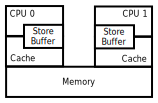
\includegraphics{memorder/SystemArchSB}}
\caption{System Architecture With Store Buffers}
\label{fig:memorder:System Architecture With Store Buffers}
\end{figure}

따라서 CPU 들은
Figure~\ref{fig:memorder:System Architecture With Store Buffers} 에 보인 것처럼
스토어 버퍼를 장착합니다.
특정 CPU 가 특정 변수에 스토어를 수행하는데 해당 변수가 해당 CPU 의 캐시에
존재하지 않는다면, 이 새로운 값은 해당 CPU 의 스토어 버퍼에 저장됩니다.
이 CPU 는 이제 이 스토어가 다른 CPU 들의 캐시들에 있을 수 있는 이 변수의 기존
값에 뭔가 작업을 수행할동안 기다리지 않고 곧바로 작업을 진행할 수 있습니다.
\iffalse

CPUs therefore come equipped with store buffers, as shown in
Figure~\ref{fig:memorder:System Architecture With Store Buffers}.
When a given CPU does a store to a variable that
is not present in that CPU's cache, then the new value
is instead placed in that CPU's store buffer.
The CPU can then proceed immediately, without having to wait for the
store to do something about all the old values of that variable
residing in other CPUs' caches.
\fi

\begin{figure}[htb]
\centering
\resizebox{3in}{!}{
\includegraphics{cartoons/r-2014-Out-of-order}}
\caption{CPUs Can Do Things Out of Order}
\ContributedBy{Figure}{fig:memorder:CPUs Can Do Things Out of Order}{Melissa Broussard}
\end{figure}

스토어 버퍼들이 성능을 상당히 향상시킬 수 있지만, 이것들은 인스트럭션들과
메모리 참조들이 비순차적으로 수행되게 만들 수 있는데, 이는 곧 심각한 혼란을
가져오게 되는데, 이 상황이
Figure~\ref{fig:memorder:CPUs Can Do Things Out of Order} 에 그려져 있습니다.
구체적으로는, 이런 스토어 버퍼들이
Listing~\ref{lst:memorder:Memory Misordering: Store-Buffering Litmus Test} 에
보인 스토어 버퍼 리트머스 테스트에 보인 잘못된 메모리 순서를 가능하게 할 수
있습니다.
\iffalse

Although store buffers can greatly increase performance,
they can cause instructions and memory references to execute out
of order, which can in turn cause serious confusion, as illustrated in
Figure~\ref{fig:memorder:CPUs Can Do Things Out of Order}.
In particular, these store buffers can cause the memory misordering
shown in the store-buffering litmus test in
Listing~\ref{lst:memorder:Memory Misordering: Store-Buffering Litmus Test}.
\fi

\begin{table*}[tbh]
\rowcolors{6}{}{lightgray}
\renewcommand*{\arraystretch}{1.1}
\small
\centering\OneColumnHSpace{-0.1in}
\begin{tabular}{rllllll}
	\toprule
	& \multicolumn{3}{c}{CPU 0} & \multicolumn{3}{c}{CPU 1} \\
	\cmidrule(l){2-4} \cmidrule(l){5-7}
	& Instruction & Store Buffer & Cache &
		Instruction & Store Buffer & Cache \\
	\cmidrule{1-1} \cmidrule(l){2-4} \cmidrule(l){5-7}
	1 & (Initial state) & & \tco{x1==0} &
		(Initial state) & & \tco{x0==0} \\
	2 & \tco{x0 = 2;} & \tco{x0==2} & \tco{x1==0} &
		\tco{x1 = 2;} & \tco{x1==2} & \tco{x0==0} \\
	3 & \tco{r2 = x1;} (0) & \tco{x0==2} & \tco{x1==0} &
		\tco{r2 = x0;} (0) & \tco{x1==2} & \tco{x0==0} \\
	4 & (Read-invalidate) & \tco{x0==2} & \tco{x0==0} &
		(Read-invalidate) & \tco{x1==2} & \tco{x1==0} \\
	5 & (Finish store) & & \tco{x0==2} &
		(Finish store) & & \tco{x1==2} \\
	\bottomrule
\end{tabular}
\caption{Memory Misordering: Store-Buffering Sequence of Events}
\label{tab:memorder:Memory Misordering: Store-Buffering Sequence of Events}
\end{table*}

Table~\ref{tab:memorder:Memory Misordering: Store-Buffering Sequence of Events}
은 이런 잘못된 메모리 접근 순서가 어떻게 일어날 수 있는지 보입니다.
Row~1 은 최초의 상태를 보이는데, 이 때 CPU~0 는 \co{x1} 을 자신의 캐시에 가지고
있고 CPU~1 은 \co{x0} 를 자기의 캐시에 가지고 있으며, 두 변수 모두 값 0을
가지고 있습니다.
Row~2 는 각 CPU 의 스토어 (
Listing~\ref{lst:memorder:Memory Misordering: Store-Buffering Litmus Test} 의
line~9 와~18) 로 인한 상태 변화를 보입니다.
두 CPU 모두 스토어가 향한 변수를 자신의 캐시에 가지고 있지 않았기에, 두 CPU 는
모두 각자의 스토어들을 자신의 스토어 버퍼들에서 처리합니다.
\iffalse

Table~\ref{tab:memorder:Memory Misordering: Store-Buffering Sequence of Events}
shows how this memory misordering can happen.
Row~1 shows the initial state, where CPU~0 has \co{x1} in its cache
and CPU~1 has \co{x0} in its cache, both variables having a value of zero.
Row~2 shows the state change due to each CPU's store (lines~9 and~18 of
Listing~\ref{lst:memorder:Memory Misordering: Store-Buffering Litmus Test}).
Because neither CPU has the stored-to variable in its cache, both CPUs
record their stores in their respective store buffers.
\fi

\QuickQuiz{}
	하지만 잠시만요!!!
	Table~\ref{tab:memorder:Memory Misordering: Store-Buffering Sequence of Events}
	의 row~2 에서 \co{x0} 와 \co{x1} 모두 동시에 두개의 값, 0 과 1 을
	가지고 있어요.
	어떻게 이게 가능한거죠???
	\iffalse

	But wait!!!
	On row~2 of
	Table~\ref{tab:memorder:Memory Misordering: Store-Buffering Sequence of Events}
	both \co{x0} and \co{x1} each have two values at the same time,
	namely zero and two.
	How can that possibly work???
	\fi
\QuickQuizAnswer{
	나중에 이야기 하겠지만, 아래쪽에 좀 더 일을 빠듯하게 처리되도록 하는
	cache-coherence 프로토콜이 존재합니다.
	하지만 어떤 변수가 동시에 두개의 값을 갖는다는게 신기하다고
	생각하신다면,
	Section~\ref{sec:memorder:Variables With Multiple Values} 까지
	잠깐 기다려 주시기 바랍니다.
	\iffalse

	There is an underlying cache-coherence protocol that straightens
	things out, which will be discussed later.
	% @@@ Add forward reference.
	But if you think that a given variable having two values at
	the same time is surprising, just wait until you get to
	Section~\ref{sec:memorder:Variables With Multiple Values}!
	\fi
} \QuickQuizEnd

Row~3 는 두개의 로드
(Listing~\ref{lst:memorder:Memory Misordering: Store-Buffering Litmus Test} 의
line~10 과~19) 를 보입니다.
각 CPU 에 의해 읽혀지는 변수들은 각 CPU 의 캐시에 있기 때문에, 각각의 로드는
곧바로 캐시의 값을 반환하는데, 이 경우 모두 0의 값입니다.

하지만 이 CPU 들은 일이 다 끝나지 않았습니다: 금방이든 나중이든, 각자의 스토어
버퍼를 비워야만 합니다.
캐시는 \emph{캐시라인 (cacheline)} 이라 불리는 상대적으로 커다란 블록 단위로
데이터를 옮기기 때문에, 그리고 각각의 캐시라인은 여러 변수들을 담고 있을 수
있기 때문에, 각 CPU 는 자신의 스토어 버퍼 안의 변수에 해당하는 캐시라인의 해당
변수에 해당하지 않는 부분은 만지지 않으면서 해당 변수에 해당하는 부분만을
업데이트 할 수 있도록 해당 캐시라인을 자신의 캐시로 가져와야만 합니다.
각 CPU 는 또한 해당 캐시라인이 어떤 다른 CPU 의 캐시에도 존재하지 않는다는 점을
보장해야만 하는데, 이를 위해 read-invalidate 오퍼레이션이 사용됩니다.
Row~4 에서 보인 것처럼, 두개의 read-invalidate 오퍼레이션이 완료된 후, 이 두
CPU 는 서로 넘겨받은 캐시라인들을 가지고 있게 되어서, CPU~0 의 캐시는 이제
\co{x0} 를 담고 있고 CPU~1 의 캐시는 \co{x1} 을 담고 있게 됩니다.
일단 이 두 변수들이 각자의 새로운 안식처에 위치하게 되면, 각 CPU 는 자신의
스토어 버퍼를 연관된 캐시 라인으로 비워낼 수 있게 되어서, 각 변수의 값을 row~5
에 보인 대로 마지막 값으로 설정합니다.
\iffalse

Row~3 shows the two loads (lines~10 and~19 of
Listing~\ref{lst:memorder:Memory Misordering: Store-Buffering Litmus Test}).
Because the variable being loaded by each CPU is in that CPU's cache,
each load immediately returns the cached value, which in both cases
is zero.

But the CPUs are not done yet: Sooner or later, they must empty their
store buffers.
Because caches move data around in relatively large blocks called
\emph{cachelines}, and because each cacheline can hold several
variables, each CPU must get the cacheline into its own cache so
that it can update the portion of that cacheline corresponding
to the variable in its store buffer, but without disturbing any
other part of the cacheline.
Each CPU must also ensure that the cacheline is not present in any other
CPU's cache, for which a read-invalidate operation is used.
As shown on row~4, after both read-invalidate operations complete,
the two CPUs have traded cachelines, so that CPU~0's cache now contains
\co{x0} and CPU~1's cache now contains \co{x1}.
Once these two variables are in their new homes, each CPU can flush
its store buffer into the corresponding cache line, leaving each
variable with its final value as shown on row~5.
\fi

\QuickQuiz{}
	하지만 이 값들은 또다시 캐시에서 메인 메모리로 비워져야 하는거
	아닌가요?
	\iffalse

	But don't the values also need to be flushed from the cache
	to main memory?
	\fi
\QuickQuizAnswer{
	놀라울 수 있겠지만, 꼭 그럴 필요는 없습니다!
	어떤 시스템들에서는, 두개의 변수들이 빈번하게 사용된다면, 이 변수들은
	CPU 의 캐시들 사이에서 움직이게 되고 메인 메모리에는 위치하지 않게
	됩니다.
	\iffalse

	Perhaps surprisingly, not necessarily!
	On some systems,
	if the two variables are being used heavily, they might
	be bounced back and forth between the CPUs' caches and never
	land in main memory.
	\fi
} \QuickQuizEnd

요약하자면, 스토어 버퍼들은 CPUe 들이 스토어 명령을 효과적으로 처리할 수 있도록
하기 위해 필요합니다만, 이게 반 직관적인, 잘못된 메모리 접근 순서를 야기할 수
있습니다.

하지만 여러분의 알고리즘이 정말로 메모리 참조의 순서를 맞춰야 한다면 어떻게
해야할까요?
예를 들어, 여러분이 어떤 드라이버와 하나는 이 드라이버가 동작 중인지 여부를 말하고 (driver-running flag) 하나는 이 드라이버에 처리되기를 기다리는 중인 요청이 있는지 여부를 말하는 (request-pending flag) 한쌍의 플래그를 사용해 통신하고 있다고 생각해 봅시다.
요청을 보내는 쪽은 request-pending flag 의 bit 을 채우고, driver-running flag 의 bit 을 검사한 후, 비어있다면 드라이버를 깨웁니다.
드라이버가 자신이 아는 모든 대기중인 요청들을 처리했다면, 드라이버는 자신의 driver-running flag 의 bit 을 없애고, 다시 일을 시작해야 하는지 여부를 보기 위해 request-pending flag 를 체크해야 합니다.
이 매우 합리적인 접근법도 하드웨어가 여기서의 스토어들과 로드들을 순서대로 처리한다고 보장할 수 있는 방법이 없다면 제대로 동작하지 않을 겁니다.
이게 다음 섹션의 주제입니다.
\iffalse

In summary, store buffers are needed to allow CPUs to handle
store instructions efficiently, but they can result in
counter-intuitive memory misordering.

But what do you do if your algorithm really needs its memory
references to be ordered?
For example, suppose that you are communicating with a driver using
a pair of flags, one that says whether or not the driver is running
and the other that says whether there is a request pending for that
driver.
The requester needs to set the request-pending flag, then check
the driver-running flag, and if false, wake it up.
Once the driver has serviced all the pending requests that it knows about,
it needs to clear its driver-running flag, then check the request-pending
flag to see if it needs to restart.
This very reasonable approach cannot work unless there is some way
to make sure that the hardware processes the stores and loads in order.
This is the subject of the next section.
\fi

\subsection{How to Force Ordering?}
\label{sec:memorder:How to Force Ordering?}

\emph{메모리 배리어} (예를 들어, 리눅스 커널의 \co{smp_mb()}) 를 사용해 순서
규칙의 환상을 지키는데 필요한 표준적 동기화 도구들 (락킹과 RCU 같은) 과
컴파일러 지시어들이 존재합니다.
이런 메모리 배리어들은 ARM, \Power{}, Itanium, 그리고 Alpha 에서처럼 명시적
인스트럭션이 될 수 있고, x86 에서 종종 그런 것처럼 다른 인스트럭션들에 의해
내포될 수도 있습니다.
이런 표준적 동기화 도구들은 순서가 지켜진다는 환상을 지키기 때문에, 여러분이
가장 쉽게 적용할 수 있는 방법은 그냥 이 도구들을 사용해서, 이 섹션을 그만 읽는
겁니다.
\iffalse

It turns out that there are compiler directives and standard
synchronization primitives (such as locking and RCU)
that are responsible for maintaining the illusion of ordering through use of
\emph{memory barriers} (for example, \co{smp_mb()} in the Linux kernel).
These memory barriers can be explicit instructions, as they are on
ARM, \Power{}, Itanium, and Alpha, or they can be implied by other instructions,
as they often are on x86.
Since these standard synchronization primitives preserve the illusion of
ordering, your path of least resistance is to simply use these primitives,
thus allowing you to stop reading this section.
\fi

\begin{listing}[tbp]
{ \scriptsize
\begin{verbbox}[\LstLineNo]
C C-SB+o-mb-o+o-mb-o
{
}

P0(int *x0, int *x1)
{
  int r2;

  WRITE_ONCE(*x0, 2);
  smp_mb();
  r2 = READ_ONCE(*x1);
}


P1(int *x0, int *x1)
{
  int r2;

  WRITE_ONCE(*x1, 2);
  smp_mb();
  r2 = READ_ONCE(*x0);
}

exists (1:r2=0 /\ 0:r2=0)
\end{verbbox}
}
\centering
\theverbbox
\caption{Memory Ordering: Store-Buffering Litmus Test}
\label{lst:memorder:Memory Ordering: Store-Buffering Litmus Test}
\end{listing}

하지만, 여러분 스스로 그런 동기화 도구들을 구현해야 한다면, 또는 그런 메모리
순서 규칙이 어떻게 동작하는지에 그저 흥미가 있는 거라면, 계속 읽어주세요!
이 여정에서의 첫번째 정류장은
Listing~\ref{lst:memorder:Memory Ordering: Store-Buffering Litmus Test}
(\path{C-SB+o-mb-o+o-mb-o.litmus}) 으로, \co{smp_mb()} 리눅스 커널 메모리
배리어가 \co{P0()} 와 \co{P1()} 의 스토어와 로드 사이에 위치했다는 점을
제외하고는
Listing~\ref{lst:memorder:Memory Misordering: Store-Buffering Litmus Test}
와 동일합니다.
이 배리어들은 제 x86 랩탑에서의 100,000,000 번의 시도에도 반 직관적인 결과가
일어나는 것을 막았습니다.
흥미롭게도, 이 배리어들로 인해 추가된 오버헤드는 두 로드가 모두 값 2 를
반환하는 경우가 800,000 번이 넘게 일어나게 만들었는데, 이는 이 배리어가 없는
Listing~\ref{lst:memorder:Memory Misordering: Store-Buffering Litmus Test} 의
코드에서는 167 번밖에 일어나지 않았던 것과 대조적입니다.
\iffalse

However, if you need to implement the synchronization primitives
themselves, or if you are simply interested in understanding how memory
ordering works, read on!
The first stop on the journey is
Listing~\ref{lst:memorder:Memory Ordering: Store-Buffering Litmus Test}
(\path{C-SB+o-mb-o+o-mb-o.litmus}),
which places an \co{smp_mb()} Linux-kernel full memory barrier between
the store and load in both \co{P0()} and \co{P1()}, but is otherwise
identical to
Listing~\ref{lst:memorder:Memory Misordering: Store-Buffering Litmus Test}.
% Test C-SB+o-mb-o+o-mb-o Allowed
% Histogram (3 states)
% 49553298:>0:r2=2; 1:r2=0;
% 49636449:>0:r2=0; 1:r2=2;
% 810253:>0:r2=2; 1:r2=2;
% No
These barriers prevent the counter-intuitive outcome from happening
on 100,000,000 trials on my x86 laptop.
Interestingly enough, the added overhead due to these barriers causes the
legal outcome where both loads return the value two to happen more
than 800,000 times, as opposed to only 167 times for the
barrier-free code in
Listing~\ref{lst:memorder:Memory Misordering: Store-Buffering Litmus Test}.
\fi

\begin{table*}[tbh]
\rowcolors{6}{}{lightgray}
\renewcommand*{\arraystretch}{1.1}
\small
\centering\OneColumnHSpace{-0.1in}
\begin{tabular}{rllllll}
	\toprule
	& \multicolumn{3}{c}{CPU 0} & \multicolumn{3}{c}{CPU 1} \\
	\cmidrule(l){2-4} \cmidrule(l){5-7}
	& Instruction & Store Buffer & Cache &
		Instruction & Store Buffer & Cache \\
	\cmidrule{1-1} \cmidrule(l){2-4} \cmidrule(l){5-7}
	1 & (Initial state) & & \tco{x1==0} &
		(Initial state) & & \tco{x0==0} \\
	2 & \tco{x0 = 2;} & \tco{x0==2} & \tco{x1==0} &
		\tco{x1 = 2;} & \tco{x1==2} & \tco{x0==0} \\
	3 & \tco{smp_mb();} & \tco{x0==2} & \tco{x1==0} &
		\tco{smp_mb();} & \tco{x1==2} & \tco{x0==0} \\
	4 & (Read-invalidate) & \tco{x0==2} & \tco{x0==0} &
		(Read-invalidate) & \tco{x1==2} & \tco{x1==0} \\
	5 & (Finish store) & & \tco{x0==2} &
		(Finish store) & & \tco{x1==2} \\
	6 & \tco{r2 = x1;} (2) & & \tco{x1==2} &
		\tco{r2 = x0;} (2) & & \tco{x0==2} \\
	\bottomrule
\end{tabular}
\caption{Memory Ordering: Store-Buffering Sequence of Events}
\label{tab:memorder:Memory Ordering: Store-Buffering Sequence of Events}
\end{table*}

이 배리어들은
Table~\ref{tab:memorder:Memory Ordering: Store-Buffering Sequence of Events} 에
보인 것과 같이 순서규칙에 깊은 영향을 끼칩니다.
앞의 두 행은
Table~\ref{tab:memorder:Memory Misordering: Store-Buffering Sequence of Events}
에 보인 것과 같고 row~3 의 \co{smp_mb()} 인스트럭션들은 직접적으로 상태를
바꾸지 않지만, 이 인스트럭션들은 스토어들이 (row~4 와~5) 로드 (row~6) 전에
완료되도록 만들어서,
Table~\ref{tab:memorder:Memory Misordering: Store-Buffering Sequence of Events}
에서 보인 반 직관적인 결과가 나타나지 못하게 합니다.
변수 \co{x0} 와 \co{x1} 은 row~2 에서 여전히 두개의 값을 갖지만, 앞서
약속한대로, 이 \co{smp_mb()} 인스턴스들은 최종적으로는 일을 더 깐깐하게
처리했음을 알아두시기 바랍니다.
\iffalse

These barriers have a profound effect on ordering, as can be seen in
Table~\ref{tab:memorder:Memory Ordering: Store-Buffering Sequence of Events}.
Although the first two rows are the same as in
Table~\ref{tab:memorder:Memory Misordering: Store-Buffering Sequence of Events}
and although the \co{smp_mb()} instructions on row~3
do not change state
in and of themselves, they do cause the stores to complete
(rows~4 and~5) before the
loads (row~6), which rules out the counter-intuitive outcome shown in
Table~\ref{tab:memorder:Memory Misordering: Store-Buffering Sequence of Events}.
Note that variables \co{x0} and \co{x1} each still have more than one
value on row~2, however, as promised earlier, the \co{smp_mb()}
instances straighten things out in the end.
\fi

\begin{table*}[tbh]
\small
\centering\OneColumnHSpace{-0.7in}
\renewcommand*{\arraystretch}{1.1}
\rowcolors{7}{lightgray}{}
\begin{tabular}{lcccccccccccc}\toprule
	& & \multicolumn{4}{c}{Prior Ordered Operation} &
		\multicolumn{7}{c}{Subsequent Ordered Operation} \\
	\cmidrule(l){3-6} \cmidrule(l){7-13}
	Operation Providing Ordering & C &
		Self & R & W & RMW & Self & R & W & DR & DW & RMW & SV \\
	\cmidrule(r){1-1} \cmidrule{2-2} \cmidrule(l){3-6} \cmidrule(l){7-13}
	Store, for example, \tco{WRITE_ONCE()} &  &
		   Y &   &   &     &      &   &   &    &    &     &  Y \\
	Load, for example, \tco{READ_ONCE()} &  &
		   Y &   &   &     &      &   &   &    &  Y &     &  Y \\
	Unsuccessful RMW operation &  &
		   Y &   &   &     &      &   &   &    &  Y &     &  Y \\
	\tco{smp_read_barrier_depends()} &  &
		     & Y &   &     &      &   &   &  Y &  Y &     &    \\
	\tco{*_dereference()} &  &
		   Y &   &   &     &      &   &   &  Y &  Y &     &  Y \\
	Successful \tco{*_acquire()} &   &
		   R &   &   &     &      & Y & Y &  Y &  Y &   Y &  Y \\
	Successful \tco{*_release()} & C &
		     & Y & Y &   Y &    W &   &   &    &    &     &  Y \\
	\tco{smp_rmb()} &   &
		     & Y &   &   R &      & Y &   &  Y &    &   R &    \\
	\tco{smp_wmb()} &   &
		     &   & Y &   W &      &   & Y &    &  Y &   W &    \\
	\tco{smp_mb()} and \tco{synchronize_rcu()} & CP &
		     & Y & Y &   Y &      & Y & Y &  Y &  Y &   Y &    \\
	Successful full-strength non-\tco{void} RMW & CP &
		   Y & Y & Y &   Y &    Y & Y & Y &  Y &  Y &   Y &  Y \\
	\tco{smp_mb__before_atomic()} & CP &
		     & Y & Y &   Y &      & a & a & a  & a  &   Y &    \\
	\tco{smp_mb__after_atomic()} & CP &
		     & a & a &   Y &      & Y & Y &  Y &  Y &     &    \\
	\bottomrule
\end{tabular}

\vspace{5pt}\hfill
\framebox[\width]{\footnotesize\setlength{\tabcolsep}{3pt}
\rowcolors{1}{}{}
\begin{tabular}{lrl}
	Key:	& C: & Ordering is cumulative \\
		& P: & Ordering propagates \\
		& R: & Read, for example, \tco{READ_ONCE()}, or read portion of RMW \\
		& W: & Write, for example, \tco{WRITE_ONCE()}, or write portion of RMW \\
		& Y: & Provides the specified ordering \\
		& a: & Provides specified ordering given intervening RMW atomic operation \\
		& DR: & Dependent read (address dependency, Section~\ref{sec:memorder:Address Dependencies}) \\
		& DW: & Dependent write (address, data, or control dependency, Sections~\ref{sec:memorder:Address Dependencies}--\ref{sec:memorder:Control Dependencies}) \\
		& RMW: & Atomic read-modify-write operation \\
		& SV: & Same-variable access \\
\end{tabular}
}\OneColumnHSpace{-0.9in}
\caption{Linux-Kernel Memory-Ordering Cheat Sheet}
\label{tab:memorder:Linux-Kernel Memory-Ordering Cheat Sheet}
\end{table*}

\co{smp_mb()} 같은 전체 배리어가 상당히 강력한 순서 보장을 갖긴 하지만, 그
강력함은 높은 비용으로부터 나옵니다.
굉장히 많은 상황들이 저렴한 메모리 순서 보장 인스트럭션을 사용하는, 또는, 어떤
경우에 있어서는, 아예 메모리 순서 보장 인스트럭션을 사용하지 않는 훨씬 약한
순서 보장만으로도 처리될 수 있습니다.
Table~\ref{tab:memorder:Linux-Kernel Memory-Ordering Cheat Sheet}
은 리눅스 커널의 순서 보장 도구들과 그 보장사항들을 보이는 커닝 페이퍼를
보입니다.
각 열은 순서 보장을 제공할 수도, 하지 않을 수도 있는 도구들 또는 도구들의
카테고리에 연관되며, ``Prior Ordered Operation'' 과 ``Subsequent Ordered
Operation'' 으로 라벨링된 행들은 각 열의 도구에 의해 순서가 맞춰지는 (또는
맞춰지지 않는) 오퍼레이션들입니다.
``Y'' 를 담는 셀들은 무조건적으로 순서가 제공됨을 의미하며, 다른 문자들은
순서가 부분적으로 또는 조건적으로 제공됨을 의미합니다.
빈 셀들은 어떤 순서 보장도 제공되지 않음을 의미합니다.
\iffalse

Although full barriers such as \co{smp_mb()} have extremely strong
ordering guarantees, their strength comes at a high price.
A great many situations can be handled with much weaker ordering guarantees
that use much cheaper memory-ordering instructions, or, in some case, no
memory-ordering instructions at all.
Table~\ref{tab:memorder:Linux-Kernel Memory-Ordering Cheat Sheet}
provides a cheatsheet of the Linux kernel's ordering primitives and their
guarantees.
Each row corresponds to a primitive or category of primitives that might
or might not provide ordering, with the columns labeled
``Prior Ordered Operation'' and ``Subsequent Ordered Operation''
being the operations that might (or might not) be ordered against.
Cells containing ``Y'' indicate that ordering is supplied unconditionally,
while other characters indicate that ordering is supplied only partially or
conditionally.
Blank cells indicate that no ordering is supplied.
\fi

\co{*_acquire} 열은 \co{smp_load_acquire()}, \co{cmpxchg_acquire()},
\co{xchg_release()}, 등등을 포함합니다;
\co{*_release} 열은 \co{smp_store_release()}, \co{cmpxchg_release()},
\co{xchg_release()}, 등등을 포함합니다; 그리고
``Successful Non-Relaxed Non-\co{void} RMW'' 열은 \co{atomic_add_return()},
\co{atomic_add_unless()}, \co{atomic_dec_and_test()}, \co{cmpxchg()},
\co{xchg()}, 등등을 포함합니다.
``Successful'' 이라는 수식어는 앞의 ``Unsuccessful RMW operation'' 행에서도
가리키듯이, 실패했을 때에는 메모리에도 순서에도 어떤 영향을 끼치지 않는
\co{atomic_add_return()}, \co{cmpxchg_acquire()}, 그리고 \co{cmpxchg_release()}
같은 도구들에 적용됩니다.
\iffalse

The \co{*_acquire} row covers \co{smp_load_acquire()},
\co{cmpxchg_acquire()}, \co{xchg_acquire()}, and so on;
the \co{*_release} row covers \co{smp_store_release()},
\co{cmpxchg_release()}, \co{xchg_release()}, and so on; and
the ``Successful full-strength non-\co{void} RMW'' row covers
\co{atomic_add_return()}, \co{atomic_add_unless()}, \co{atomic_dec_and_test()},
\co{cmpxchg()}, \co{xchg()}, and so on.
The ``Successful'' qualifiers apply to primitives such as
\co{atomic_add_unless()}, \co{cmpxchg_acquire()}, and \co{cmpxchg_release()},
which have no effect on either memory or on ordering when they indicate
failure, as indicated by the earlier ``Unsuccessful RMW operation'' row.
\fi

``C'' 행은 누적성과 전파성을 의미하는데, 이에 대해서는
Sections~\ref{sec:memorder:Cumulativity}
과~\ref{sec:memorder:Propagation} 에서 설명됩니다.
해당 섹션을 읽기 전까지는, 이 행은 최대 두개 쓰레드만이 돌아가는 상황에서는
대부분 무시될 수 있다는 정도만 알아두면 되겠습니다.
\iffalse

Column ``C'' indicates cumulativity and propagation, as explained in
Sections~\ref{sec:memorder:Cumulativity}
and~\ref{sec:memorder:Propagation}.
In the meantime, this column can usually be ignored when there
are at most two threads involved.
\fi

\QuickQuiz{}
	Table~\ref{tab:memorder:Linux-Kernel Memory-Ordering Cheat Sheet}
	의 열들은 상당히 무작위적이고 복잡해 보입니다.
	이 표의 개념적 근본이 무엇인가 있나요?
	\iffalse

	The rows in
	Table~\ref{tab:memorder:Linux-Kernel Memory-Ordering Cheat Sheet}
	seem quite random and confused.
	Whatever is the conceptual basis of this table???
	\fi
\QuickQuizAnswer{
	각 열들은 전력과 오버헤드가 증가되는 하드웨어 메커니즘들에 대략적으로
	연관되어 있습니다.

	\co{WRITE_ONCE()} 행은 ``SV'' 열로 표시되듯이 하나의 변수로의 액세스는
	항상 완벽히 순서잡힌다는 사실을 사용합니다.
	특졍 변수에 순서를 제공하는 모드 다른 오퍼레이션들도 이 같은 변수로의
	순서를 제공함을 알아 두시기 바랍니다.

	\co{READ_ONCE()} 열은 (2017 년에 있어) 컴파일러들과 CPU 들은 사용자가
	볼 수 있는 예측적 스토어를 탐닉하지 않아서, 주소, 데이터, 또는 수행이
	앞의 로드에 의존적인 모든 스토어는 해당 로드가 완료된 후에 행해진다는
	사실을 사용합니다.
	최소한 이런 의존성들이
	Sections~\ref{sec:memorder:Address- and Data-Dependency Restrictions}
	과~\ref{sec:memorder:Control-Dependency Restrictions} 에서 설명된 대로
	주의깊게 구성되었다는 가정 아래의 이야기입니다.
	\iffalse

	The rows correspond roughly to hardware mechanisms of increasing
	power and overhead.

	The \co{WRITE_ONCE()} row captures the fact that accesses to
	a single variable are always fully ordered, as indicated by
	the ``SV''column.
	Note that all other operations providing ordering against an
	access to a
	specific variable also provide this same-variable ordering.

	The \co{READ_ONCE()} row captures the fact that (as of 2017) compilers
	and CPUs do not indulge in user-visible speculative stores, so that
	any store whose address, data, or execution depends on a prior load
	will happen after that load completes.
	At least assuming that these dependencies have been constructed
	carefully as described in
	Sections~\ref{sec:memorder:Address- and Data-Dependency Restrictions}
	and~\ref{sec:memorder:Control-Dependency Restrictions}.
	\fi

	``Unsuccessful RMW operation'' 열은 실패한 RMW 라 하더라도 읽기는 하게
	되고, 그 읽기는 \co{READ_ONCE()} 만큼은 좋은 효과를 낸다는 사실을
	사용합니다.

	\co{smp_read_barrier_depends()} 열은 DEC Alpha 의 예외가 있긴 하지만,
	컴파일러들과 CPU 들은 사용자가 볼 수 있는 주소 의존성들은 깨지 않는다는
	사실을 사용하는데, 역시 이 의존성들이
	Section~\ref{sec:memorder:Address- and Data-Dependency Restrictions}
	에서 설명한 대로 주의 깊게 구성되었다는 가정 하이긴 합니다.

	\co{*_dereference()} 열은 \co{lockless_dereference()},
	\co{rcu_dereference()}, 등등에 의해 제공되는 주소와 데이터 종속성 순서
	규칙을 사용합니다.

	``Successful \co{*_acquire()}'' 열은 많은 CPU 가 특별한 ``acquire''
	형태의 로드와 atomic RMW 인스트럭션들을 가지고 있으며, 많은 다른 CPU 가
	앞의 로드들을 뒤의 로드들과 스토어들에 대해 순서 맞춰주는 가벼운 메모리
	배리어 인스트럭션을 가지고 있다는 사실을 사용합니다.
	\iffalse

	The ``Unsuccessful RMW operation'' row captures the fact that
	even an unsuccessful RMW has done a read, and that read is
	every bit as good as a \co{READ_ONCE()}.

	The \co{smp_read_barrier_depends()} row captures the fact that, with the
	notable exception of DEC Alpha, compilers and CPUs do not indulge
	in user-visible breakage of address dependencies, again assuming
	that these dependencies have been constructed carefully as described in
	Section~\ref{sec:memorder:Address- and Data-Dependency Restrictions}.

	The \co{*_dereference()} row captures the address and data
	dependency ordering provided by \co{lockless_dereference()},
	\co{rcu_dereference()}, and friends.

	The ``Successful \co{*_acquire()}'' row captures the fact that many
	CPUs have special ``acquire'' forms of loads and of atomic RMW
	instructions,
	and that many other CPUs have light-weight memory-barrier
	instructions that order prior loads against subsequent loads
	and stores.
	\fi

	``Successful \co{*_release()}'' 열은 많은 CPU 가 특수한 ``release''
	형태의 store 와 atomic RMW 인스트럭션들을 가지고 있으며, 많은 다른 CPU
	가 앞의 로드들을 뒤따르는 스토어들에 대해 순서맞춰주는 가벼운 메모리
	배리어 인스트럭션들을 가지고 있다는 사실을 사용합니다.

	\co{smp_rmb()} 열은 많은 CPU 들이 앞의 로드들을 뒤따르는 로드들에 대해
	순서맞춰주는 가벼운 메모리 배리어 인스트럭션들을 가지고 있다는 사실을
	사용합니다.
	비슷하게,
	\co{smp_wmb()} 열은 많은 CPU 들이 앞의 스토어들을 뒤따른 스토어들에
	대해 순서맞춰주는 가벼운 메모리 배리어 인스트럭션들을 가지고 있다는
	사실을 사용합니다.
	\iffalse

	The ``Successful \co{*_release()}'' row captures the fact that many
	CPUs have special ``release'' forms of stores and of atomic RMW
	instructions, and that many other CPUs have light-weight memory-barrier
	instructions that order prior loads and stores against
	subsequent stores.

	The \co{smp_rmb()} row captures the fact that many CPUs have
	light-weight memory-barrier instructions that order prior loads against
	subsequent loads.
	Similarly,
	the \co{smp_wmb()} row captures the fact that many CPUs have
	light-weight memory-barrier instructions that order prior stores against
	subsequent stores.
	\fi

	따라서 이 순서 맞추기 오퍼레이션들 중 어느것도 앞의 스토어들이 뒤따르는
	로드들에 대해 순서맞춰줄 것을 요구하지 않는데, 이는 이 오퍼레이션들이
	앞의 스토어들을 뒤따르는 로드들에 대해 재배치하는 게 삶의 목표인 스토어
	버퍼에 간섭하지 않는다는 것을 의미합니다.
	이런 오퍼레이션들의 비용이 가벼운 것은 이 오퍼레이션들의 스토어 버퍼에
	간섭하지 않는다는 정책 덕분입니다.

	\co{smp_mb()} 열은 Itanium 의 예외가 있지만 대부분의 플랫폼에서 사용
	가능한 전체 메모리 배리어에 연관됩니다.

	``Successful Non-Relaxed None-\co{void} RMW'' 열은 (x86 과 같은) 일부
	플랫폼에서 atomic RMW 인스트럭션들은 그 앞과 뒤 사이에 전체 순서 규칙을
	제공한다는 사실을 사용합니다.
	따라서 리눅스 커널은 full-streangth non-\co{void} atomic RMW 오퍼레이션들이 이
	오퍼레이션들이 성공한 경우에 대해서는 전체 순서 규칙을 제공할 것을
	요구합니다.
	(full-streangth atomic RMW 오퍼레이션의 이름들은 \co{_relaxed},
	\co{_acquire}, 또는 \co{_relaxed} 로 끝나지 않습니다.)
	\iffalse

	None of the ordering operations thus far require prior stores to be
	ordered against subsequent loads, which means that these operations
	need not interfere with store buffers, whose main purpose in life
	is in fact to reorder prior stores against subsequent loads.
	The light-weight nature of these operations is precisely due to
	their policy of store-buffer non-interference.
	However, as noted earlier, it is sometimes necessary to interfere
	with the store buffer in order to prevent prior stores from being
	reordered against later stores, which brings us to the remaining
	rows in this table.

	The \co{smp_mb())} row corresponds to the full memory barrier
	available on most platforms, with Itanium being the exception
	that proves the rule.

	The ``Successful full-strength non-\co{void} RMW'' row captures
	the fact that on some platforms (such as x86) atomic RMW instructions
	provide full ordering both before and after.
	The Linux kernel therefore requires that full-strength non-\co{void}
	atomic RMW operations provide full ordering in cases where these
	operations succeed.
	(Full-strength atomic RMW operation's names do not end in
	\co{_relaxed}, \co{_acquire}, or \co{_release}.)
	\fi

	하지만, 리눅스 커널은 \co{atomic_inc()} 와 같은 \co{void} atomic RMW
	오퍼레이션들에 대해서는 어떠한 순서 보장도 제공할 것을 요구하지
	않습니다.
	따라서, 이 오퍼레이션들과 실패한 non-\co{void} atomic RMW
	오퍼레이션들은 앞의, 또는 뒤의 메모리 액세스 모두에 대해 완전한 순서를
	보장하기 위해 \co{smp_mb__before_atomic()} 을 앞세우고 뒤에
	\co{smp_mb__before_atomic()} 을 뒤에 배치해야 할 겁니다.
	이 표의 \co{smp_mb__before_atomic()} 과 \co{smp_mb__after_atomic()}
	열의 ``a'' 항목이 이야기 하듯이, \co{smp_mb__before_atomic()} (또는,
	유사하게, \co{smp_mb__after_atomic()}) 과 atomic RMW 오퍼레이션
	사이에서는 어떤 메모리 접근에 대해서도 순서 보장을 제공할 필요가
	없습니다.

	요약해서, 이 테이블에서의 모든 무작위성은 그 아래에 위치한,
	Chapter~\ref{chp:Hardware and its Habits} 에서 앞서 설명된 대로 물리
	법칙에 의해서만 제약되는 하드웨어의 특성 탓입니다.
	\iffalse

	However, the Linux kernel does not require that \co{void} atomic
	RMW operations provide any ordering whatsoever, with the
	canonical example being \co{atomic_inc()}.
	Therefore, these operations, along with failing non-\co{void}
	atomic RMW operations may be preceded by \co{smp_mb__before_atomic()}
	and followed by \co{smp_mb__after_atomic()} to provide full
	ordering for any accesses preceding or following both.
	No ordering need be provided for accesses between the
	\co{smp_mb__before_atomic()} (or, similarly, the
	\co{smp_mb__after_atomic()}) and the atomic RMW operation, as
	indicated by the ``a'' entries on the \co{smp_mb__before_atomic()}
	and \co{smp_mb__after_atomic()} rows of the table.

	In short, any randomness in the table is due to the properties
	of the underlying hardware, which are constrained by nothing other
	than the laws of physics, as was explained back in
	Chapter~\ref{chp:Hardware and its Habits}.
	\fi
	% forward reference to rf co fr section
} \QuickQuizEnd

이 표는 단지 컨닝 페이퍼에 불과하며, 따라서 메모리 순서 규칙에 대한 제대로 된
이해를 대체할 수는 없습니다.
그런 이해를 세우기 시작하기 위해, 다음 섹션은 일부 경험에 의거한 규칙들을
소개합니다.
\iffalse

It is important to note that this table is just a cheat sheet,
and is therefore in no way a replacement for a good understanding
of memory ordering.
To begin building such an understanding, the next section will
present some basic rules of thumb.
\fi

\subsection{Basic Rules of Thumb}
\label{sec:memorder:Basic Rules of Thumb}

이 섹션은 매우 많은 상황에 대해 ``훌륭하고 충분한'' 기본적인 경험으로부터의
법칙들을 소개합니다.
사실, 여러분은 이 경험으로부터의 법칙들 외에는 어떤 것도 필요치 않은 채 훌륭한
성능과 확장성을 갖는 동시성 코드를 대부분 작성할 수 있습니다.
\iffalse

This section presents some basic rules of thumb that are ``good and
sufficient'' for a great many situations.
In fact, you could write a great deal of concurrent code having
excellent performance and scalability without needing anything more
than these rules of thumb.
\fi

\QuickQuiz{}
	하지만 특정 프로젝트가 이 경험으로부터의 법칙들의 범위 내에서 설계되고
	코딩 될 수 있다고 알 수 있죠?
	\iffalse

	But how can I know that a given project can be designed
	and coded within the confines of these rules of thumb?
	\fi
\QuickQuizAnswer{
	이 챕터의 나머지 부분들의 대부분의 목적은 정확히 이 질문에 답하는
	것입니다!
	\iffalse

	Much of the purpose of the remainder of this chapter is
	to answer exactly that question!
	\fi
} \QuickQuizEnd

\paragraph{A given thread sees its own accesses in order.}
이 규칙은 공유된 변수에 대한 로드와 스토어가 각각 \co{READ_ONCE()} 와
\co{WRITE_ONCE()} 를 사용한다는 것을 가정합니다.
그러지 않는다면, 컴파일러가 여러분의 코드를 바닥부터 휘저을 수 있고\footnote{
	많은 컴파일러 개발자들이 ``휘젓는다'' 대신 ``최적화'' 라는 단어를
	선호합니다만, 우리 모두 각자의 선호하는 것이 있지요.}, 가끔은 CPU 역시
조금은 코드를 휘저을 수 있습니다.
\iffalse

This rule assumes that loads and stores from/to shared variables use
\co{READ_ONCE()} and \co{WRITE_ONCE()}, respectively.
Otherwise, the compiler can profoundly scramble\footnote{
	Many compiler writers prefer the word ``optimize'' instead of
	``scramble'', but we all have our preferences.}
your code, and sometimes the CPU can do a bit of scrambling as well.
\fi
% @@@ Itanium forward reference?

\begin{figure}[htb]
\centering
\resizebox{3in}{!}{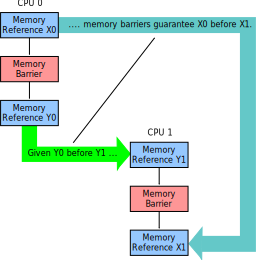
\includegraphics{memorder/memorybarrier}}
\caption{Memory Barriers Provide Conditional If-Then Ordering}
\label{fig:memorder:Memory Barriers Provide Conditional If-Then Ordering}
\end{figure}

\paragraph{Ordering has conditional if-then semantics.}
Figure~\ref{fig:memorder:Memory Barriers Provide Conditional If-Then Ordering}
는 메모리 배리어들을 위한 이 규칙을 보입니다.
두 메모리 배리어가 모두 충분히 강력하다 가정하고 (확신이 서지 않는다면, 언제든
\co{smp_mb()} 를 사용하세요), 만약 CPU~1 의 액세스 Y1 이 CPU~0 의 액세스 Y0
뒤에 일어났다면, CPU~1 의 액세스 X1 은 CPU~0 의 액세스 X1 뒤에 일어날 것이
보장됩니다.
\iffalse

Figure~\ref{fig:memorder:Memory Barriers Provide Conditional If-Then Ordering}
illustrates this for memory barriers.
Assuming that both memory barriers are strong enough (and when in doubt, you
can always use \co{smp_mb()}), if CPU~1's access Y1 happens after CPU~0's
access Y0, then CPU~1's access X1 is guaranteed to happen after CPU~0's
access X1.
\fi

\QuickQuiz{}
	특정 상황에서 어떤 메모리 배리어들이 충분히 강력한지 어떻게 이야기 할
	수 있나요?
	\iffalse

	How can you tell which memory barriers are strong enough for
	a given use case?
	\fi
\QuickQuizAnswer{
	아, 그건 답변하는데 이 챕터의 나머지 부분의 대부분을 필요로 할 만큼
	깊은 질문입니다.
	\iffalse

	Ah, that is a deep question whose answer requires most of the
	rest of this chapter.
	\fi
} \QuickQuizEnd

Listing~\ref{lst:memorder:Memory Ordering: Store-Buffering Litmus Test}
은 이 점에서의 한 예입니다.
Line~10 과~20 에서의 \co{smp_mb()} 는 배리어들의 역할을, line~9 에서의 \co{x0}
스토어는 X0 역할을, line~11 에서의 \co{x1} 으로부터의 로드는 Y0 를, line~19
에서의 \co{x1} 스토어는 Y1, 그리고 \co{x0} 로부터의 로드는 X1 역할을 합니다.
이 if-then 규칙을 단계별로 적용해 보면, 만약 \co{P0()} 의 로컬 변수 \co{r2} 가
값 0으로 설정되어 있다면 line~19 에서의 \co{x1} 스토어는 line~11 에서의 \co{x1}
로드 뒤에 일어났음을 알 수 있습니다.
그렇다면 이 if-then 규칙은 line~21 에서의 \co{x0} 으로부터의 로드가 line~9 의
\co{x0} 으로의 스토어 뒤에 일어났음을 이야기할 것입니다.
달리 말하자면,
\emph{만약} \co{P0()} 의 로컬 변수 \co{r2} 가 값 0으로 끝난다면 \co{P1()} 의
로컬 변수 \co{r2} 는 값 2로 끝날 것이 보장됩니다.
다시 말하지만, 메모리 순서 보장은 조건적이지, 절대적이지 않습니다.
\iffalse

Listing~\ref{lst:memorder:Memory Ordering: Store-Buffering Litmus Test}
is a case in point.
The \co{smp_mb()} on line~10 and~20 serve as the barriers,
the store to \co{x0} on line~9 as X0, the load from \co{x1} on line~11
as Y0, the store to \co{x1} on line~19 as Y1, and the load from
\co{x0} as X1.
Applying the if-then rule step by step, we know that the store to
\co{x1} on line~19 happens after the load from \co{x1} on line~11 if
\co{P0()}'s local variable \co{r2} is set to the value zero.
The if-then rule would then state that the load from \co{x0} on
line~21 happens after the store to \co{x0} on line~9.
In other words,
\co{P1()}'s local variable \co{r2} is guaranteed
to end up with the value two \emph{only if}
\co{P0()}'s local variable \co{r2} ends up with the value zero.
Again, memory ordering guarantees are conditional, not absolute.
\fi

비록
Figure~\ref{fig:memorder:Memory Barriers Provide Conditional If-Then Ordering}
가 구체적으로 메모리 배리어들을 언급하지만, 리눅스 커널의 나머지 순서 보장
오퍼레이셔들에도 같은 규칙이 적용됩니다.
\iffalse

Although
Figure~\ref{fig:memorder:Memory Barriers Provide Conditional If-Then Ordering}
specifically mentions memory barriers, the same rule applies to the
rest of the Linux kernel's ordering operations.
\fi

\paragraph{Ordering operations must be paired.}
여러분이 한 쓰레드에서의 오퍼레이션들의 순서는 주의깊게 맞췄지만, 다른
쓰레드에서는 그렇게 하는데 실패했다면, 순서가 없게 됩니다.
두 쓰레드 모두 앞의 if-then 규칙이 적용될 수 있도록 순서를 제공해야만
합니다.\footnote{
	Section~\ref{sec:memorder:Propagation} 에서, 짝 맞추기는 사이클로
	일반화 될겁니다.}
\iffalse

If you carefully order the operations in one thread, but then fail to do
so in another thread, then there is no ordering.
Both threads must provide ordering for the if-then rule to apply.\footnote{
	In Section~\ref{sec:memorder:Propagation}, pairing will be
	generalized to cycles.}
\fi

\paragraph{Ordering operations almost never speed things up.}
앞의 스토어가 메모리에 더 빨리 적용될 수 있도록 강제하기 위해 메모리 배리어를
추가하려 하고 있다면, 참으세요!
순서 보장을 추가하는건 일반적으로 일을 느려지게 만듭니다.
물론, 인스트럭션들을 추가하는 것이 일을 더 빨리 처리되게 만드는 경우도
있습니다만, 그런 경우에는 주의깊은 벤치마킹이 필요합니다.
그리고 설령 그렇다 하더라도, 여러분이 \emph{여러분의} 시스템에서 조금 속도를
높일 수 있었다 할지라도, 여러분의 사용자들의 시스템들에서는 상당히 속도가
떨어지는 경우가 있을 가능성도 있습니다.
또는 여러분의 미래의 시스템에서요.
\iffalse

If you find yourself tempted to add a memory barrier in an attempt
to force a prior store to be flushed to memory faster, resist!
Adding ordering usually slows things down.
Of course, there are situations where adding instructions speeds things
up, but careful benchmarking is required in such cases.
And even then, it is quite possible that although you sped things up
a little bit on \emph{your} system, you might well have slowed things
down significantly on your users' systems.
Or on your future system.
\fi

\paragraph{Ordering operations are not magic.}
여러분의 프로그램이 어떤 레이스 컨디션으로 문제가 발생한다면, 여러분의 버그가
존재하지 않도록 하기 위해 몇가지 메모리 순서 보장 오퍼레이션들을 추가하고
싶어지는 경우가 많을 겁니다.
이보다 훨씬 나은 반응은 주의깊게 설계된 형태로 더 높은 단계의 기능들을 사용하는
것입니다.
동시성 프로그래밍에서, 여러분의 버그들을 존재하지 않게 설계하는게 존재하지
않도록 꼼수를 부리는 것보다 거의 항상 쉽습니다!
\iffalse

When your program is failing due to some race condition, it is often
tempting to toss in a few memory-ordering operations in an attempt
to barrier your bugs out of existence.
A far better reaction is to use higher-level primitives in a carefully
designed manner.
With concurrent programming, it is almost always easier to design
your bugs out of existence than to hack them out of existence!
\fi

\paragraph{These are only rough rules of thumb.}
비록 이 경험으로부터의 규칙들이 실제 현업에서 보여지는 대부분의 상황들을 다룰
수 있긴 하지만, 모든 경험으로부터의 규칙들이 그러하듯이 이 규칙들 역시 한계가
있습니다.
다음 섹션은 여러분의 직관을 깨부수고 여러분의 이해를 높여줄 trick-and-trap
리트머스 테스트들을 소개함으로써 이 한계들을 일부 보이겠습니다.
이 리트머시 테스트들은 또한
Table~\ref{tab:memorder:Linux-Kernel Memory-Ordering Cheat Sheet}
로 보여진 리눅스 커널 메모리 순셔규칙 커닝 페이퍼로 나타내어지는 개념들을
명확하게 할겁니다.
Section~\ref{sec:memorder:Where is Memory Ordering Needed?} 은 모든 트릭들과
함정들로부터 배운 것들을 가지고 이 커닝 페이퍼를 다시 한번 들여다 볼 겁니다.
\iffalse

Although these rules of thumb cover the vast majority of situations
seen in actual practice, as with any set of rules of thumb, they
do have their limits.
The next section will demonstrate some of these limits by introducing
trick-and-trap litmus tests that are intended to insult your
intuition while increasing your understanding.
These litmus tests will also illuminate many of the concepts
represented by the Linux-kernel memory-ordering cheat sheet shown in
Table~\ref{tab:memorder:Linux-Kernel Memory-Ordering Cheat Sheet}.
Section~\ref{sec:memorder:Where is Memory Ordering Needed?} will
circle back to this cheat sheet in light of learnings from all the
intervening tricks and traps.
\fi

\section{Tricks and Traps}
\label{sec:memorder:Tricks and Traps}

이제 하드웨어가 메모리 액세스 순서를 재배치 할 수 있고 여러분은 그걸 막을 수
있음을 알게 되었으니, 다음은 여러분이 여러분의 직관에 문제가 있음을 인정하도록
할 차례입니다.
이 고통스러운 작업은 scalar 변수들이 동시에 여러 값들을 가지고 있음을 보이는
코드를 소개하는
Section~\ref{sec:memorder:Variables With Multiple Values}, 그리고
직관적으로 올바르지만 실제 하드웨어에서는 비참하게 실패하고 마는 코드들을
보이는
Sections~\ref{sec:memorder:Memory-Reference Reordering} 부터
\ref{sec:memorder:Multicopy Atomicity} 까지를 통해 이루어질 겁니다.
이 비탄의 작업을 통해 일단 여러분의 직관이 만들어지면, 뒤의 섹션들에서 우리가
근간으로 삼게 될, 메모리 배리어들이 따르는 기본 규칙들을 제공합니다.
이 규칙들은 더 나아가

하지만 먼저, 한 순간에 하나의 변수가 얼마나 많은 값들을 가지고 있을 수 있는지
간단히 알아봅시다.
\iffalse

Now that you know that hardware can reorder memory accesses and that you
can prevent it from doing so, the next step is to get you to admit
that your intuition has a problem.
This painful task is taken up by
Section~\ref{sec:memorder:Variables With Multiple Values},
which presents some code demonstrating that scalar variables can
take on multiple values simultaneously,
and by
Sections~\ref{sec:memorder:Memory-Reference Reordering} through
\ref{sec:memorder:Multicopy Atomicity},
which show a series of intuitively correct code fragments that fail miserably
on real hardware.
Once your intuition has made it through the grieving process, later
sections will summarize the basic rules that memory ordering follows.

But first, let's take a quick look at just how many values a single
variable might have at a single moment of time.
\fi

\subsection{Variables With Multiple Values}
\label{sec:memorder:Variables With Multiple Values}

하나의 변수는 잘 정의된 전역적 순서로 값들의 연속을 갖게 될 거라 생각하는건
자연스럽습니다.
불행히도, 이 여정의 다음 정류장은 이 편안한 거짓에 ``작별''을 고하라 합니다.
바라건대, 여러분은 이미
Tables~\ref{tab:memorder:Memory Misordering: Store-Buffering Sequence of Events}
와~\ref{tab:memorder:Memory Ordering: Store-Buffering Sequence of Events} 의
row~2 를 통해 ``작별'' 을 고하기 시작했을 것이고 만약 그렇다면 이 섹션의 목적은
이 요점을 제대로 이끌어내는 것입니다.
\iffalse

It is natural to think of a variable as taking on a well-defined
sequence of values in a well-defined, global order.
Unfortunately, the next stop on the journey says ``goodbye'' to this comforting fiction.
Hopefully, you already started to say ``goodbye'' in response to row~2 of
Tables~\ref{tab:memorder:Memory Misordering: Store-Buffering Sequence of Events}
and~\ref{tab:memorder:Memory Ordering: Store-Buffering Sequence of Events},
and if so, the purpose of this section is to drive this point home.
\fi

그러기 위해,
Listing~\ref{lst:memorder:Software Logic Analyzer} 에 보인 프로그램의 한 부분을
고려해 봅시다.
이 코드 조각은 여러 CPU 들에서 병렬적으로 수행됩니다.
Line~1 은 하나의 공유 변수를 현재 CPU 의 ID 로 값을 할당하고, line~2 에서는
모든 CPU 들 가운데 동기화 되는 (불행히도, 모든 CPU 구조에서 가능한 일은
아닙니다!) 하드웨어 ``timebase'' 카운터의 값을 가져오는 \co{gettb()} 함수를
사용해 일부 변수들을 초기화 시키고, line~3-8 의 루프에서는 이 CPU 가 할당한
값이 유지된 시간의 길이를 기록합니다.
물론, 이 CPU 들 가운데 하나는 ``승리'' 할 것이고, 따라서 line~6-7 의 검사가
아니라면 이 루프를 절대 빠져나오지 않을 겁니다.
\iffalse

To this end, consider the program fragment shown in
Listing~\ref{lst:memorder:Software Logic Analyzer}.
This code fragment is executed in parallel by several CPUs.
Line~1 sets a shared variable to the current CPU's ID, line~2
initializes several variables from a \co{gettb()} function that
delivers the value of a fine-grained hardware ``timebase'' counter that is
synchronized among all CPUs (not available from all CPU architectures,
unfortunately!), and the loop from lines~3-8 records the length of
time that the variable retains the value that this CPU assigned to it.
Of course, one of the CPUs will ``win'', and would thus never exit
the loop if not for the check on lines~6-7.
\fi

\QuickQuiz{}
	Listing~\ref{lst:memorder:Software Logic Analyzer}
	의 코드에서의 어떤 가정이 실제 하드웨어에서는 성립하지 않을까요?
	\iffalse

	What assumption is the code fragment
	in Listing~\ref{lst:memorder:Software Logic Analyzer}
	making that might not be valid on real hardware?
	\fi
\QuickQuizAnswer{
	이 코드는 특정 CPU 가 자신의 값을 보는 것을 멈추자마자, 곧바로
	마지막으로 동의된 값을 보게 될 것이라 가정삽니다.
	실제 하드웨어에서, 어떤 CPU 들은 이 마지막 값을 보게 되기 전에 중간의
	결과를 일부 보게 될수도 있습니다.
	따라서 이 섹션의 뒤에서 이야기될 그림들의 데이터를 만드는데 사용된 실제
	코드는 좀 더 복잡합니다.
	\iffalse

	The code assumes that as soon as a given CPU stops
	seeing its own value, it will immediately see the
	final agreed-upon value.
	On real hardware, some of the CPUs might well see several
	intermediate results before converging on the final value.
	The actual code used to produce the data in the figures
	discussed later in this section was therefore somewhat more
	complex.
	\fi
} \QuickQuizEnd

\begin{listing}[tbp]
{ \scriptsize
\begin{verbbox}
  1 state.variable = mycpu;
  2 lasttb = oldtb = firsttb = gettb();
  3 while (state.variable == mycpu) {
  4   lasttb = oldtb;
  5   oldtb = gettb();
  6   if (lasttb - firsttb > 1000)
  7     break;
  8 }
\end{verbbox}
}
\centering
\theverbbox
\caption{Software Logic Analyzer}
\label{lst:memorder:Software Logic Analyzer}
\end{listing}

루프를 빠져나오기 전, \co{firsttb} 는 앞의 공유 변수에의 값 할당 후 곧바로
가져온 timestamp 를 가지고 있을 것이고 \co{lasttb} 는 여전히 할당된 값을 가지고
있을, 이 공유 변수의 마지막 샘플링 전에 가져온 timestamp 를 가지고 있을 수도
있고, 만약 이 공유 변수가 루프에 들어오기 전에 바뀌었다면 \co{firsttb} 와 같은
값을 가지고 있을 수도 있습니다.
이는 우리가 532-나노세컨드의 시간 간격 동안의 각 CPU 의 \co{state.variable} 의
값에 대한 관찰을 그려볼 수 있게 해주는데,
Figure~\ref{fig:memorder:A Variable With Multiple Simultaneous Values} 에
보여져 있습니다.
이 데이터는 2006년에 각각 두개의 하드웨어 쓰레드를 갖는 8개의 코어를 장착한
1.5\,GHz \Power{5} 시스템에서 수집되었습니다.
CPU~1, 2, 3, 그리고~4 는 이 값들을 기록했고, CPU~0 는 이 테스트를 제어했습니다.
Timebase 카운터의 시간 간격은 5.32\,ns 정도였는데, 이는 중간의 캐시 상태들을
관찰하기에 충분히 작은 간격입니다.
\iffalse

Upon exit from the loop, \co{firsttb} will hold a timestamp
taken shortly after the assignment and \co{lasttb} will hold
a timestamp taken before the last sampling of the shared variable
that still retained the assigned value, or a value equal to \co{firsttb}
if the shared variable had changed before entry into the loop.
This allows us to plot each CPU's view of the value of \co{state.variable}
over a 532-nanosecond time period, as shown in
Figure~\ref{fig:memorder:A Variable With Multiple Simultaneous Values}.
This data was collected in 2006 on 1.5\,GHz \Power{5} system with 8 cores,
each containing a pair of hardware threads.
CPUs~1, 2, 3, and~4 recorded the values, while CPU~0 controlled the test.
The timebase counter period was about 5.32\,ns, sufficiently fine-grained
to allow observations of intermediate cache states.
\fi

\begin{figure}[htb]
\centering
\resizebox{3in}{!}{\includegraphics{memorder/MoreThanOneValue}}
\caption{A Variable With Multiple Simultaneous Values}
\label{fig:memorder:A Variable With Multiple Simultaneous Values}
\end{figure}

각각의 수평의 막대는 해당 CPU 의 관찰 결과를 시간대별로 보여주는데, 왼쪽 검은
영역은 해당 CPU 의 첫번째 관측 전까지의 시간을 나타냅니다.
처음 5\,ns 동안, CPU~3 만이 이 변수의 값을 읽었습니다.
그 다음 10\,ns 동안, CPU~2 와~3 은 이 변수의 값을 서로 다르게 이야기했는데, 그
후에는 최종적으로 동의된 값인 ``2'' 라는 값에 합의했습니다.
하지만, CPU~1 은 이 값이 ``1'' 이라고 거의 300\,ns 동안 믿었고, CPU~4 는 거의
500\,ns 동안이나 이 값이 ``4'' 라고 믿었습니다.
\iffalse

Each horizontal bar represents the observations of a given CPU over time,
with the gray regions to the left indicating the time before the
corresponding CPU's first measurement.
During the first 5\,ns, only CPU~3 has an opinion about the value of the
variable.
During the next 10\,ns, CPUs~2 and~3 disagree on the value of the variable,
but thereafter agree that the value is~``2'', which is in fact
the final agreed-upon value.
However, CPU~1 believes that the value is~``1'' for almost 300\,ns, and
CPU~4 believes that the value is~``4'' for almost 500\,ns.
\fi

\QuickQuiz{}
	어떻게 CPU 들이 하나의 변수를 \emph{동시에} 서로 다르게 볼 수가
	있는거죠?
	\iffalse

	How could CPUs possibly have different views of the
	value of a single variable \emph{at the same time?}
	\fi
\QuickQuizAnswer{
	Section~\ref{sec:memorder:Why Hardware Misordering?}
	에서 논의된 대로, 많은 CPU 들이 최근의 스토어 값을 기록하는 스토어
	버퍼를 가지고 있으며, 이 값은 연관된 캐시 라인이 해당 CPU 로 올라오기
	전에는 외부에 보여지지 않습니다.
	따라서, 각 CPU 가 하나의 시점에 특정 변수에 대해 서로 다른 값을 보고
	있는 것이---그리고 메인 메모리는 또 다른 값을 가지고 있는 것이
	가능합니다.
	메모리 배리어가 발명된 이유들 중 하나는 소프트웨어가 이런 종류의 상황을
	우아하게 처리할 수 있도록 해주기 위함이었습니다.
	\iffalse

	As discussed in
	Section~\ref{sec:memorder:Why Hardware Misordering?},
	many CPUs have store buffers that record the values of
	recent stores, which do not become globally visible until
	the corresponding cache line makes its way to the CPU.
	Therefore, it is quite possible for each CPU to see a
	different value for a given variable at a single point
	in time---and for main memory to hold yet another value.
	One of the reasons that memory barriers were invented was
	to allow software to deal gracefully with situations like
	this one.
	\fi
} \QuickQuizEnd

\QuickQuiz{}
	CPU~1 과~4 는 값을 동의하는데에 그렇게 오랜 시간이 걸렸는데, CPU~2 와~3
	은 어떻게 그렇게 빨리 값에 동의하는 건가요?
	\iffalse

	Why do CPUs~2 and~3 come to agreement so quickly, when it
	takes so long for CPUs~1 and~4 to come to the party?
	\fi
\QuickQuizAnswer{
	CPU~2 와~3 은 같은 코어의 하드웨어 쓰레드들이어서 같은 캐시 계층을
	공유하며, 따라서 매우 낮은 통신 응답시간을 갖습니다.
	이게 NUMA, 또는, 보다 정확히는, NUCA 효과입니다.

	이는 CPU~2 와~3 가 왜 값에 대해 동의하지 않는 순간이 존재하긴 하는가에
	대한 질문을 떠올리게 합니다.
	가능한 한가지 이유는 이들이 커다란 공유된 캐시 외에 작은 개별 캐시를
	갖고 있을 수 있다는 것입니다.
	여기서의 짧은 10-나노세컨드 동안의 비동의된 시간과 해당 코드에 메모리
	순서 강제 오퍼레이션이 아예 없었다는 것을 놓고 보면, 또다른 가능할 법한
	이유는 인스트럭션 재배치입니다.
	\iffalse

	CPUs~2 and~3 are a pair of hardware threads on the same
	core, sharing the same cache hierarchy, and therefore have
	very low communications latencies.
	This is a NUMA, or, more accurately, a NUCA effect.

	This leads to the question of why CPUs~2 and~3 ever disagree
	at all.
	One possible reason is that they each might have a small amount
	of private cache in addition to a larger shared cache.
	Another possible reason is instruction reordering, given the
	short 10-nanosecond duration of the disagreement and the
	total lack of memory-ordering operations in the code fragment.
	\fi
} \QuickQuizEnd

그리고 네개의 CPU 에서의 상황이 재밌다고 생각한다면, 같은 상황을 15~CPU 들이
각각 시간 $t=0$ 에 하나의 공유 변수에 각자의 숫자를 할당하는 경우를 보인
Figure~\ref{fig:memorder:A Variable With More Simultaneous Values} 를 고려해
보세요.
해당 그림의 두 다이어그램은 모두
Figure~\ref{fig:memorder:A Variable With Multiple Simultaneous Values} 와 같은
방식으로 그려졌습니다.
유일한 차이점은 가로축의 단위가 timebase tick 으로, 각 tick 은 약
5.3~나노세컨드를 의미합니다.
따라서 여기서의 전체 연속된 값의 변화는 CPU 의 수의 증가에 일관되게
Figure~\ref{fig:memorder:A Variable With Multiple Simultaneous Values} 에서보다
긴 시간동안 유지되었습니다.
위의 다이어그램은 전체 그림을 보이며, 아래쪽의 것은 첫 50~timebase tick 만을
확대해서 보입니다.

여기서도, CPU~0 는 테스트를 제어했고, 따라서 어떤 값도 기록하지 않았습니다.
\iffalse

And if you think that the situation with four CPUs was intriguing, consider
Figure~\ref{fig:memorder:A Variable With More Simultaneous Values},
which shows the same situation, but with 15~CPUs each assigning their
number to a single shared variable at time~$t=0$. Both diagrams in the
figure are drawn in the same way as
Figure~\ref{fig:memorder:A Variable With Multiple Simultaneous Values}.
The only difference is that the unit of horizontal axis is timebase ticks,
with each tick lasting about 5.3~nanoseconds.
The entire sequence therefore lasts a bit longer than the events recorded in
Figure~\ref{fig:memorder:A Variable With Multiple Simultaneous Values},
consistent with the increase in number of CPUs.
The upper diagram shows the overall picture, while the lower one shows
the zoom-up of first 50~timebase ticks.

Again, CPU~0 coordinates the test, so does not record any values.
\fi

\begin{figure*}
\centering
\resizebox{5in}{!}{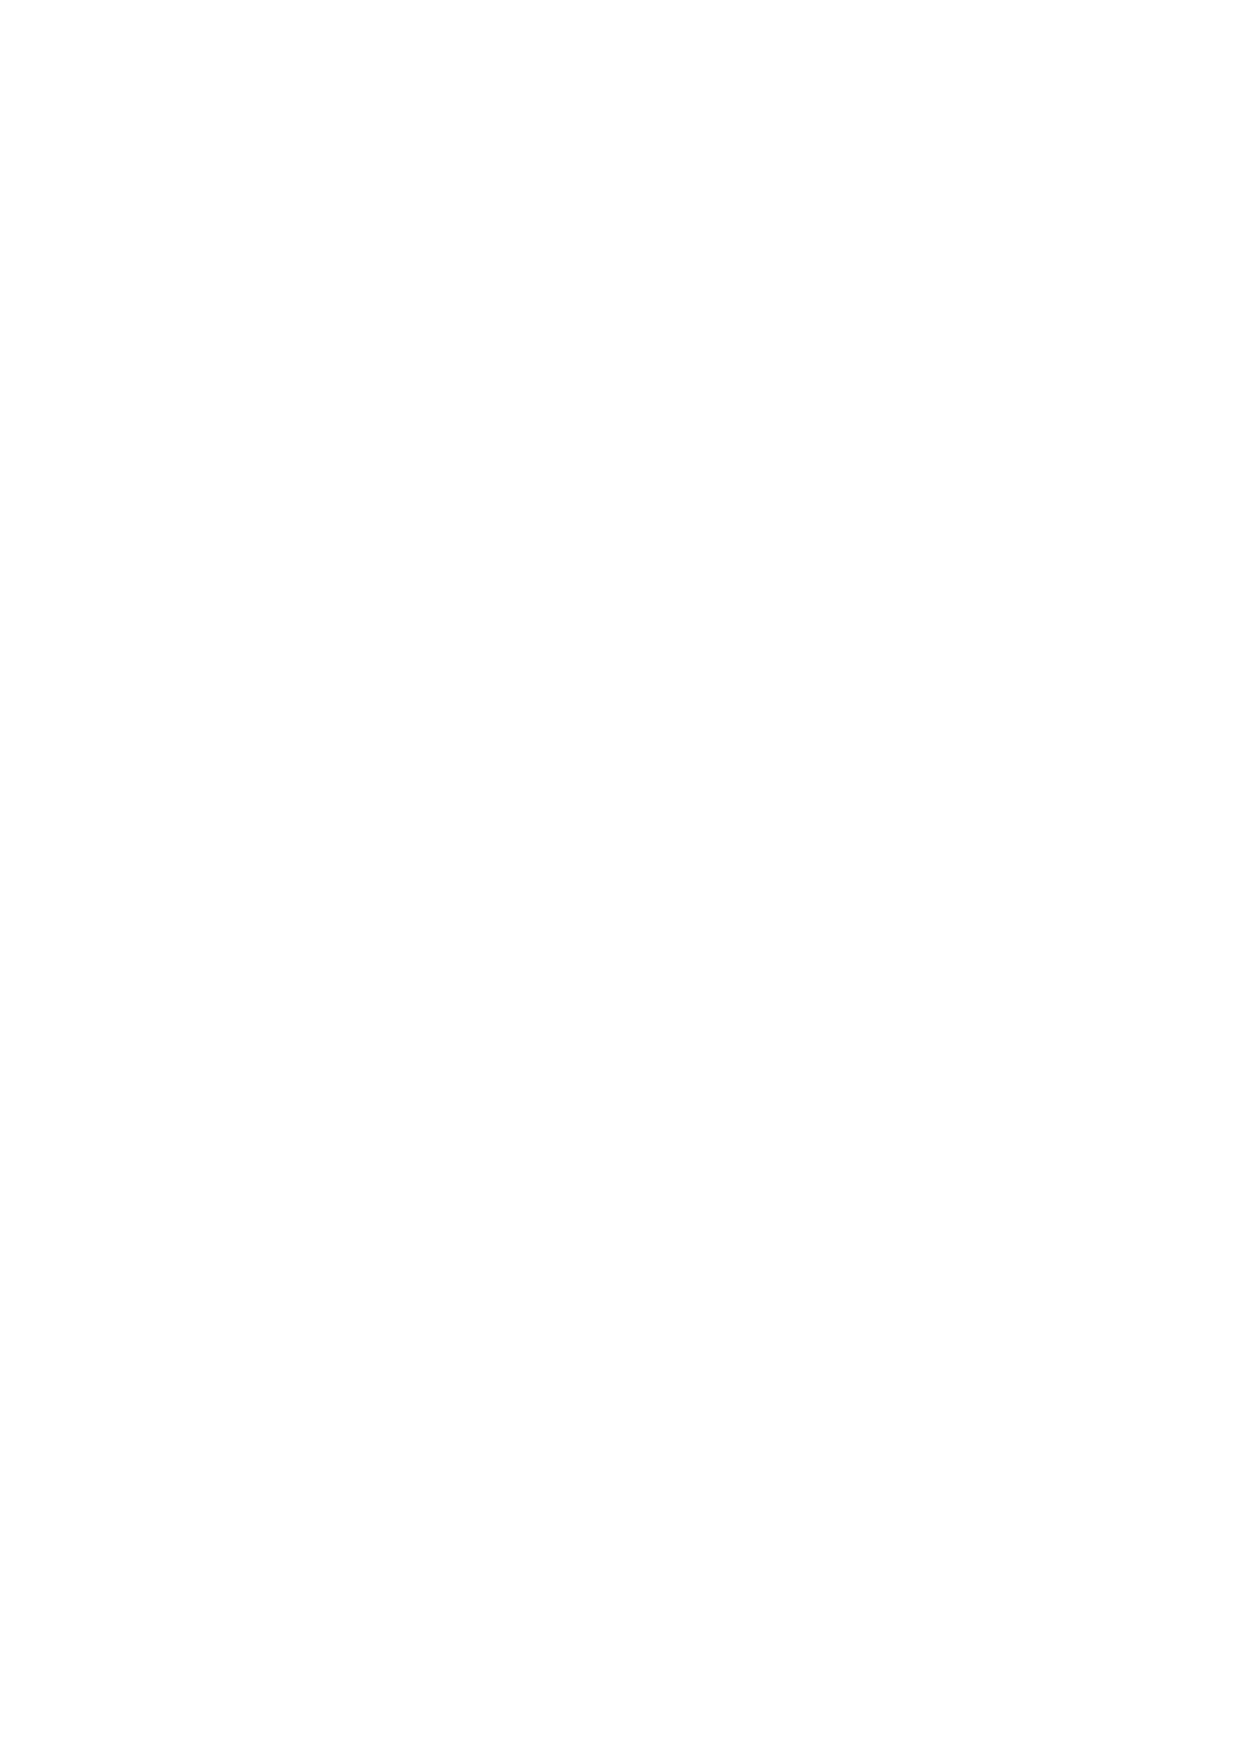
\includegraphics{memorder/MoreThanOneValue-15CPU}}
\caption{A Variable With More Simultaneous Values}
\ContributedBy{Figure}{fig:memorder:A Variable With More Simultaneous Values}{Akira Yokosawa}
\end{figure*}

모든 CPU 들이 결국은 마지막 값~9 에 동의를 합니다만, 값~15 와 값~12 가 먼저
상황을 이끈 후입니다.
아래쪽 다이어그램의 수직선으로 나타내어진 time~21 시점에 변수의 값에 대한
14개의 서로 다른 의견들이 존재했음을 알아두시기 바랍니다.
또한 모든 CPU 들이 값들의 순서에 대해
Figure~\ref{fig:memorder:Possible Global Orders With More Simultaneous Values}
에 보인 방향성 있는 그래프의 순서와 일관된 순서를 보았음을 알아두시기 바랍니다.
더도 아니고 덜도 아니고, 두 그림은 메모리 접근 순서에 신경 쓰는 코드에서의
메모리 배리어 같은 메모리 순서 보장 오퍼레이션들의 올바른 사용의 중요성을
강조합니다.
\iffalse

All CPUs eventually agree on the final value of~9, but not before
the values~15 and~12 take early leads.
Note that there are fourteen different opinions on the variable's value
at time~21 indicated by the vertical line in the lower diagram.
Note also that all CPUs see sequences whose orderings are consistent with
the directed graph shown in
Figure~\ref{fig:memorder:Possible Global Orders With More Simultaneous Values}.
Nevertheless, both figures underscore the importance of
proper use of memory-ordering operations, such as memory barriers,
for code that cares about memory ordering.
\fi

\begin{figure}[htb]
\centering
\resizebox{2.0in}{!}{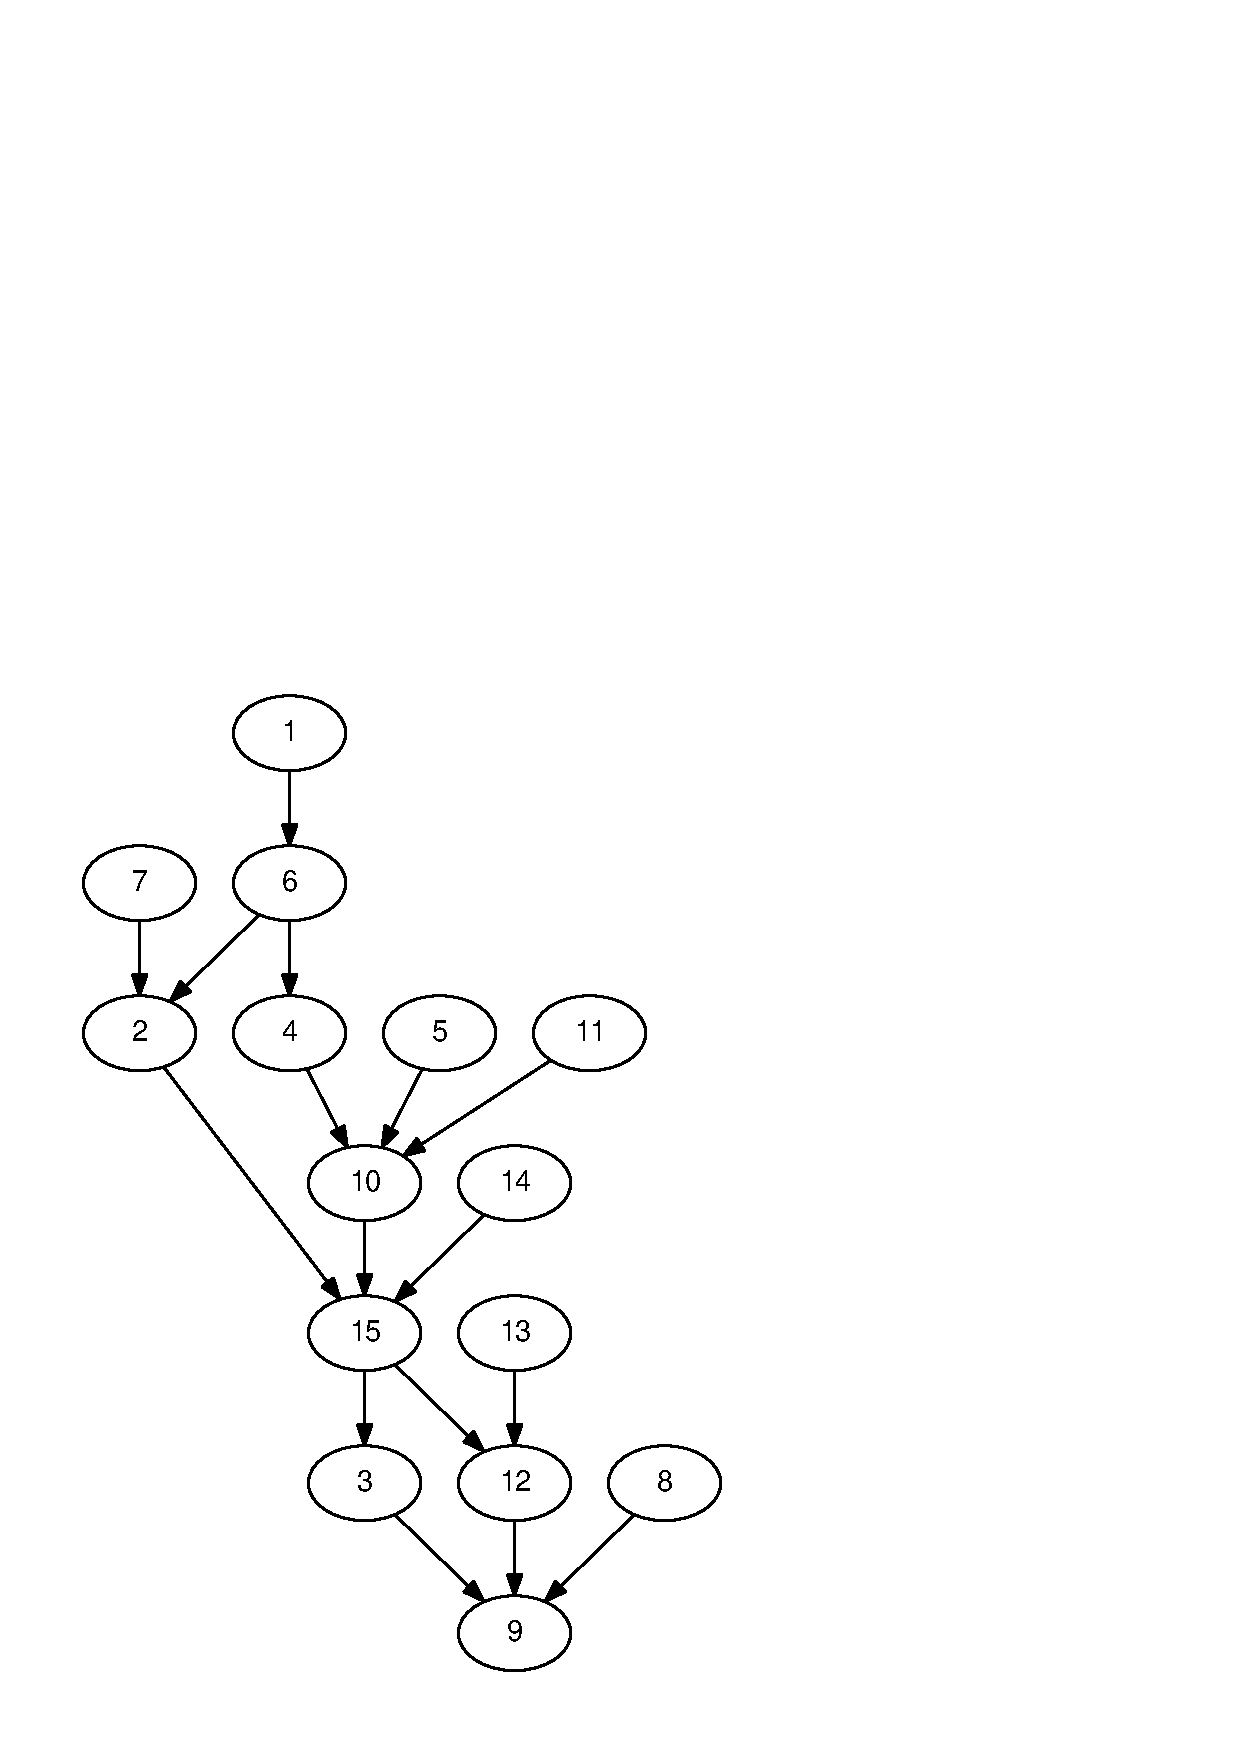
\includegraphics{memorder/store15tred}}
\caption{Possible Global Orders With More Simultaneous Values}
\label{fig:memorder:Possible Global Orders With More Simultaneous Values}
\end{figure}

하나의 변수는 한 시점에 얼마나 많은 값들을 가질 수 있을까요?
시스템에 존재하는 스토어 버퍼 하나당 하나씩입니다!
따라서 우리는 변수들의 값들과 시간의 흐름에 대한 편안한 직관에게 작별을
고해야만 하는 체제에 들어섰습니다.
이는 메모리 순서 보장 오퍼레이션들이 필요한 체제입니다.

이와 함께,
Chapter~\ref{chp:Hardware and its Habits}
와~\ref{cha:Partitioning and Synchronization Design} 에서 배웠던 교훈들을
기억할 필요가 있습니다.
모든 CPU 들이 같은 변수에게 동시에 스토어를 하도록 하는 것은 병렬 프로그램을
설계하는 방법이 아닌데, 적어도 성능과 확장성이 여러분에게 전혀 중요하지 않은 게
아니라면 그렇습니다.

불행히도, 메모리 순서 규칙은 여러분의 직관을 망칠 수 있는 방법들을 이외에도
많이 가지고 있으며, 이런 방법들 모두가 성능과 확장성을 훼손하는 건 아닙니다.
다음 섹션은 관계없는 메모리 참조의 순서 재배치에 대한 소개를 제공합니다.
\iffalse

How many values can a single variable take on at a single point in
time?
As many as one per store buffer in the system!
We have therefore entered a regime where we must bid a fond farewell to
comfortable intuitions about values of variables and the passage of time.
This is the regime where memory-ordering operations are needed.

All that aside, it is important to remember the lessons from
Chapters~\ref{chp:Hardware and its Habits}
and~\ref{cha:Partitioning and Synchronization Design}.
Having all CPUs store concurrently to the same variable
is absolutely no way to design a parallel program, at least
not if performance and scalability are at all important to you.

Unfortunately, memory ordering has many other ways of insulting your
intuition, and not all of these ways conflict with performance and
scalability.
The next section will give an overview of reordering of unrelated
memory reference.
\fi

\subsection{Memory-Reference Reordering}
\label{sec:memorder:Memory-Reference Reordering}

Section~\ref{sec:memorder:Why Hardware Misordering?}
에서는 x86 과 같이 상대적으로 강력한 순서 규칙의 시스템들도 앞의 스토어들을
뒤의 로드들과 만약 이 스토어와 로드가 서로 다른 변수들에 대해 행해진다면 재배치
시킬 수 있다는 것을 보였습니다.
이 섹션은 이 결과에 기반해서, 다른 로드와 스토어 조합을 봅니다.
\iffalse

Section~\ref{sec:memorder:Why Hardware Misordering?}
showed that even relatively strongly ordered systems like x86
can reorder prior stores with later loads, at least when the
store and load are to different variables.
This section builds on that result, looking at the other combinations of
loads and stores.
\fi

% @@@ Rationale for further reordering.

\begin{listing}[tbp]
{ \scriptsize
\begin{verbbox}[\LstLineNo]
C C-MP+o-wmb-o+o-o

{
}


P0(int* x0, int* x1) {

  WRITE_ONCE(*x0, 2);
  smp_wmb();
  WRITE_ONCE(*x1, 2);

}

P1(int* x0, int* x1) {

  int r2;
  int r3;

  r2 = READ_ONCE(*x1);
  r3 = READ_ONCE(*x0);

}

exists (1:r2=2 /\ 1:r3=0)
\end{verbbox}
}
\centering
\theverbbox
\caption{Message-Passing Litmus Test (No Ordering)}
\label{lst:memorder:Message-Passing Litmus Test (No Ordering)}
\end{listing}

\subsubsection{Load Followed By Load}
\label{sec:memorder:Load Followed By Load}

Listing~\ref{lst:memorder:Message-Passing Litmus Test (No Ordering)}
(\path{C-MP+o-wmb-o+o-o.litmus})
는 고전적 \emph{message-passing} 리트머스 테스트를 보이는데, 여기서 \co{x0} 는
메세지이고 \co{x1} 은 메세지가 존재하는지 여부를 알리는 플래그입니다.
이 테스트에서, \co{smp_wmb()} 는 \co{P0()} 의 스토어들이 순서대로 행해지게
강제하지만, 로드들에 대해서는 어떤 순서도 강제하지 않습니다.
x86 과 같이 상대적으로 강력한 순서 규칙의 아키텍쳐들에서는 순서를 강제합니다.
하지만, 완화된 순서 규칙의 아키텍쳐들은 그렇지 않은 경우가
많습니다~\cite{JadeAlglave2011ppcmem}.
따라서, 이 listing 의 line~25 에서의 \co{exists} 절은 발동될 수
\emph{있습니다}.
\iffalse

Listing~\ref{lst:memorder:Message-Passing Litmus Test (No Ordering)}
(\path{C-MP+o-wmb-o+o-o.litmus})
shows the classic \emph{message-passing} litmus test, where \co{x0} is
the message and \co{x1} is a flag indicating whether or not a message
is available.
In this test, the \co{smp_wmb()} forces \co{P0()} stores to be ordered,
but no ordering is specified for the loads.
Relatively strongly ordered architectures, such as x86, do enforce ordering.
However, weakly ordered architectures often do
not~\cite{JadeAlglave2011ppcmem}.
Therefore, the \co{exists} clause on line~25 of the listing \emph{can}
trigger.
\fi

\begin{listing}[tbp]
{ \scriptsize
\begin{verbbox}[\LstLineNo]
C C-MP+o-wmb-o+o-rmb-o

{
}

P0(int* x0, int* x1) {

  WRITE_ONCE(*x0, 2);
  smp_wmb();
  WRITE_ONCE(*x1, 2);

}

P1(int* x0, int* x1) {

  int r2;
  int r3;

  r2 = READ_ONCE(*x1);
  smp_rmb();
  r3 = READ_ONCE(*x0);

}

exists (1:r2=2 /\ 1:r3=0)
\end{verbbox}
}
\centering
\theverbbox
\caption{Enforcing Order of Message-Passing Litmus Test}
\label{lst:memorder:Enforcing Order of Message-Passing Litmus Test}
\end{listing}

따라서, 이 경우에 순서에 의존적이고 완화된 순서규칙의 아키텍쳐에도 이식될 수
있을 법한 코드에서는 명시적인 순서 규칙을 추가해야 하는데, 예를 들면
Listing~\ref{lst:memorder:Enforcing Order of Message-Passing Litmus Test}
(\path{C-MP+o-wmb-o+o-rmb-o.litmus})
의 line~20 에 보인, \co{exists} 절이 발동될 수 없게 하는 \co{smp_rmb()} 를
추가하는 식입니다.
\iffalse

Thus, portable code relying on ordering in this case must
add explicit ordering, for example, the \co{smp_rmb()} shown on
line~20 of
Listing~\ref{lst:memorder:Enforcing Order of Message-Passing Litmus Test}
(\path{C-MP+o-wmb-o+o-rmb-o.litmus}), which prevents
the \co{exists} clause from triggering.
\fi

\begin{listing}[tbp]
{ \scriptsize
\begin{verbbox}[\LstLineNo]
C C-LB+o-o+o-o
{
}

P0(int *x0, int *x1)
{
  int r2;

  r2 = READ_ONCE(*x1);
  WRITE_ONCE(*x0, 2);
}


P1(int *x0, int *x1)
{
  int r2;

  r2 = READ_ONCE(*x0);
  WRITE_ONCE(*x1, 2);
}

exists (1:r2=2 /\ 0:r2=2)
\end{verbbox}
}
\centering
\theverbbox
\caption{Load-Buffering Litmus Test (No Ordering)}
\label{lst:memorder:Load-Buffering Litmus Test (No Ordering)}
\end{listing}

\subsubsection{Load Followed By Store}
\label{sec:memorder:Load Followed By Store}

Listing~\ref{lst:memorder:Load-Buffering Litmus Test (No Ordering)}
(\path{C-LB+o-o+o-o.litmus})
은 고전적인 \emph{load-buffering} 리트머스 테스트를 보입니다.
x86 이나 IBM Mainframe 과 같이 비교적 강력한 순서규칙을 가진 시스템들은 앞의
로드들을 뒤따르는 스토어들과 재배치 하지 않지만, 더 완화된 순서 규칙의
아키텍쳐들은 그런 재배치를 정말로 허용합니다~\cite{JadeAlglave2011ppcmem}.
따라서, line~22 의 \co{exists} 절은 정말로 발동될 수 있습니다.
\iffalse

Listing~\ref{lst:memorder:Load-Buffering Litmus Test (No Ordering)}
(\path{C-LB+o-o+o-o.litmus})
shows the classic \emph{load-buffering} litmus test.
Although relatively strongly ordered systems such as x86
or the IBM Mainframe do not reorder prior loads with subsequent stores,
more weakly ordered architectures really do allow such
reordering~\cite{JadeAlglave2011ppcmem}.
Therefore, the \co{exists} clause on line~22 really can trigger.
\fi

\begin{listing}[tbp]
{ \scriptsize
\begin{verbbox}[\LstLineNo]
C C-LB+o-r+a-o
{
}

P0(int *x0, int *x1)
{
  int r2;

  r2 = READ_ONCE(*x1);
  smp_store_release(x0, 2);
}


P1(int *x0, int *x1)
{
  int r2;

  r2 = smp_load_acquire(x0);
  WRITE_ONCE(*x1, 2);
}

exists (1:r2=2 /\ 0:r2=2)
\end{verbbox}
}
\centering
\theverbbox
\caption{Enforcing Ordering of Load-Buffering Litmus Test}
\label{lst:memorder:Enforcing Ordering of Load-Buffering Litmus Test}
\end{listing}

실제 하드웨어가 이런 재배치를 하는건 비교적 드문
일이긴 합니다만~\cite{LucMaranget2017aarch64},
이식성 있는 코드는 더도 말고 덜도 말고
Listing~\ref{lst:memorder:Enforcing Ordering of Load-Buffering Litmus Test}
(\path{C-LB+o-r+a-o.litmus})
에 보인 것과 같이 모든 필요한 순서 규칙을 강제해야만 합니다.
이는 line~22 의 \co{exists} 절이 절대 발동되지 않을 것을 보장합니다.
\iffalse

Although it is rare for actual hardware to
exhibit this reordering~\cite{LucMaranget2017aarch64},
portable code must nevertheless enforce any required ordering, for example,
as shown in
Listing~\ref{lst:memorder:Enforcing Ordering of Load-Buffering Litmus Test}
(\path{C-LB+o-r+a-o.litmus}).
This guarantees that the \co{exists} clause on line~22 never triggers.
\fi

\begin{listing}[tbp]
{ \scriptsize
\begin{verbbox}[\LstLineNo]
C C-MP+o-o+o-rmb-o

{
}

P0(int* x0, int* x1) {

  WRITE_ONCE(*x0, 2);
  WRITE_ONCE(*x1, 2);

}

P1(int* x0, int* x1) {

  int r2;
  int r3;

  r2 = READ_ONCE(*x1);
  smp_rmb();
  r3 = READ_ONCE(*x0);

}

exists (1:r2=2 /\ 1:r3=0)
\end{verbbox}
}
\centering
\theverbbox
\caption{Message-Passing Litmus Test, No Writer Ordering (No Ordering)}
\label{lst:memorder:Message-Passing Litmus Test, No Writer Ordering (No Ordering)}
\end{listing}

\subsubsection{Store Followed By Store}
\label{sec:memorder:Store Followed By Store}

Listing~\ref{lst:memorder:Message-Passing Litmus Test, No Writer Ordering (No Ordering)}
(\path{C-MP+o-o+o-rmb-o.litmus})
은 다시 한번 고전적 메세지 패싱 리트머스 테스트를 보이는데, 이번에는 \co{P0()}
로의 스토어들에 대한 명시적 순서가 없고 \co{P1()} 의 로드들에 대한 순서가
\co{smp_rmb()} 로 제공되어진 버전입니다.
다시 한번 말하지만, 상대적으로 강력한 순서 규칙의 아키텍쳐들은 순서를
지켜주지만, 완화된 순서 규칙의 아키텍쳐들은 그러지 않기
때문에~\cite{JadeAlglave2011ppcmem}, \co{exists} 절은 발동될 수 있습니다.
따라서, 이식성 있는 코드는
Listing~\ref{lst:memorder:Enforcing Order of Message-Passing Litmus Test} 에서
보인 것과 같이 스토어들에도 명시적 순서를 부여해서 \co{exists} 절이 발동되지
않게 해야만 합니다.
\iffalse

Listing~\ref{lst:memorder:Message-Passing Litmus Test, No Writer Ordering (No Ordering)}
(\path{C-MP+o-o+o-rmb-o.litmus})
once again shows the classic message-passing litmus test, but without
explicit ordering for \co{P0()}'s stores and with the \co{smp_rmb()}
providing ordering for \co{P1()}'s loads.
Again, the relatively strongly ordered architectures do enforce ordering,
but weakly ordered architectures do not necessarily do
so~\cite{JadeAlglave2011ppcmem}, which means that the
\co{exists} clause can trigger.
Therefore, portable code must explicitly order the stores, for
example, as shown in
Listing~\ref{lst:memorder:Enforcing Order of Message-Passing Litmus Test},
thus preventing the \co{exists} clause from triggering.
\fi

\subsection{Address Dependencies}
\label{sec:memorder:Address Dependencies}

\emph{Address dependency} 는 로드 인스트럭션에 의해 리턴된 값이 나중의 메모리
레퍼런스 인스트럭션에 의해 사용되는 주소의 계산에 사용될 때 발생합니다.
\iffalse

An \emph{address dependency} occurs when the value returned by a load
instruction is used to compute the address used by a later memory-reference
instruction.
\fi

\begin{listing}[tbp]
{ \scriptsize
\begin{verbbox}[\LstLineNo]
C C-MP+o-wmb-o+o-addr-o

{
int y=1;
int *x1 = &y;
}

P0(int* x0, int** x1) {

  WRITE_ONCE(*x0, 2);
  smp_wmb();
  WRITE_ONCE(*x1, x0);

}

P1(int** x1) {

  int *r2;
  int r3;

  r2 = READ_ONCE(*x1);
  r3 = READ_ONCE(*r2);

}

exists (1:r2=x0 /\ 1:r3=1)
\end{verbbox}
}
\centering
\theverbbox
\caption{Message-Passing Address-Dependency Litmus Test (No Ordering)}
\label{lst:memorder:Message-Passing Address-Dependency Litmus Test (No Ordering)}
\end{listing}

Listing~\ref{lst:memorder:Message-Passing Address-Dependency Litmus Test (No Ordering)}
(\path{C-MP+o-wmb-o+o-addr-o.litmus})
은 message-passing 패턴의 링크 버전을 보입니다.
헤드 포인터는 \co{x1} 으로, 최초에 \co{int} 변수 \co{y} 를 가리키게 되며
(line~5), 변수 \co{y} 는 초기값 $1$ 을 갖습니다 (line~4).
\co{P0()} 는 헤드 포인터 \co{x1} 이 \co{x0} 를 가리키도록 업데이트 (line~12)
하는데 이는 \co{x0} 가 $2$ 로 초기화 (line~10) 된 후로 순서지어집니다
(line~11).
\co{P1()} 은 헤드 포인터 \co{x1} 을 가져오고 (line~21) 이를 통해 레퍼런스되는
값을 가져옵니다 (line~22).
따라서 line~21 의 로드와 line~22 의 로드 사이에는 address dependency 가
존재합니다.
이 경우에, line~21 에서 리턴되는 값은 line~22 에서 사용되는 주소값 그
자체이지만, C-언어의 \co{->} 오퍼레이터를 사용한 필드 접근, 더하기, 빼기,
그리고 배열 인덱싱 등 많은 변종이 있을 수 있습니다.
\iffalse

Listing~\ref{lst:memorder:Message-Passing Address-Dependency Litmus Test (No Ordering)}
(\path{C-MP+o-wmb-o+o-addr-o.litmus})
shows a linked variant of the message-passing pattern.
The head pointer is \co{x1}, which initially
references the \co{int} variable \co{y} (line~5), which is in turn
initialized to the value $1$ (line~4).
\co{P0()} updates head pointer \co{x1} to reference \co{x0} (line~12),
but only afer initializing it to $2$ (line~10) and forcing ordering
(line~11).
\co{P1()} picks up the head pointer \co{x1} (line~21), and then loads
the referenced value (line~22).
There is thus an address dependency from the load on line~21 to the
load on line~22.
In this case, the value returned by line~21 is exactly the address
used by line~22, but many variations are possible,
including field access using the C-language \co{->} operator,
addition, subtraction, and array indexing.
\fi

어떤 사람들은 line~21 의 헤드 포인터 로드가 line~22 의 dereference 전으로 순서
잡히길 바랄 겁니다.
하지만,
Section~\ref{sec:memorder:Alpha} 에서 설명할, 종속적 로드에 대한 예측된 값의
사용을 할 수 있는 DEC Alpha 에서는 그렇지 않을 겁니다.
따라서,
Listing~\ref{lst:memorder:Message-Passing Address-Dependency Litmus Test (No Ordering)}
의 \co{exists} 절은 발동될 수 \emph{있습니다}.
\iffalse

One might hope that line~21's load from the head pointer would be ordered
before line~22's dereference.
However, this is not the case on DEC Alpha, which can in effect use
a speculated value for the dependent load, as described in more detail in
Section~\ref{sec:memorder:Alpha}.
Therefore,
Listing~\ref{lst:memorder:Message-Passing Address-Dependency Litmus Test (No Ordering)}'s
\co{exists} clause \emph{can} trigger.
\fi

\begin{listing}[tbp]
{ \scriptsize
\begin{verbbox}[\LstLineNo]
C C-MP+o-wmb-o+ld-addr-o

{
int y=1;
int *x1 = &y;
}

P0(int* x0, int** x1) {

  WRITE_ONCE(*x0, 2);
  smp_wmb();
  WRITE_ONCE(*x1, x0);

}

P1(int** x1) {

  int *r2;
  int r3;

  r2 = lockless_dereference(*x1);
  r3 = READ_ONCE(*r2);

}

exists (1:r2=x0 /\ 1:r3=1)
\end{verbbox}
}
\centering
\theverbbox
\caption{Enforced Ordering of Message-Passing Address-Dependency Litmus Test}
\label{lst:memorder:Enforced Ordering of Message-Passing Address-Dependency Litmus Test}
\end{listing}

Listing~\ref{lst:memorder:Enforced Ordering of Message-Passing Address-Dependency Litmus Test}
(\path{C-MP+o-wmb-o+ld-addr-o.litmus})
은 DEC Alpha 도 포함해서 이식성 있게 동작하도록 어떻게 할 수 있는지 보이는데,
line~21 의 \co{READ_ONCE()} 를 \co{lockless_dereference()} 로 대체하는 것으로,
\co{lockless_dereference()} 는 DEC Alpha 외의 모든 플랫폼에서 \co{READ_ONCE()}
와 동일하지만, DEC Alpha 에서는 \co{READ_ONCE()} 뒤에 \co{smp_mb()} 를 붙여
동작해서 모든 플랫폼에서 필요한 순서규칙을 강제하고, 결국 \co{exists} 절이
발동되지 않게 해줍니다.
\iffalse

Listing~\ref{lst:memorder:Enforced Ordering of Message-Passing Address-Dependency Litmus Test}
(\path{C-MP+o-wmb-o+ld-addr-o.litmus})
shows how to make this work portably, even on DEC Alpha, by
replacing line~21's \co{READ_ONCE()} with \co{lockless_dereference()},
which acts like \co{READ_ONCE()} on all platforms other than DEC Alpha,
where it acts like a \co{READ_ONCE()} followed by an \co{smp_mb()},
thereby forcing the required ordering on all platforms, in turn
preventing the \co{exists} clause from triggering.
\fi

\begin{listing}[tbp]
{ \scriptsize
\begin{verbbox}[\LstLineNo]
C C-S+o-wmb-o+o-addr-o

{
int y=1;
int *x1 = &y;
}

P0(int* x0, int** x1) {

  WRITE_ONCE(*x0, 2);
  smp_wmb();
  WRITE_ONCE(*x1, x0);

}

P1(int** x1) {

  int *r2;

  r2 = READ_ONCE(*x1);
  WRITE_ONCE(*r2, 3);

}

exists (1:r2=x0 /\ x0=2)
\end{verbbox}
}
\centering
\theverbbox
\caption{S Address-Dependency Litmus Test}
\label{lst:memorder:S Address-Dependency Litmus Test}
\end{listing}

하지만, 예를 들어,
Listing~\ref{lst:memorder:S Address-Dependency Litmus Test}
(\path{C-S+o-wmb-o+o-addr-o.litmus}) 에 보인 \emph{S} 리트머스
테스트~\cite{JadeAlglave2011ppcmem} 와 같이 종속적 오퍼레이션이 로드가 아니라
스토어라면 어떻게 될까요?
어떤 제품 품질의 플랫폼도 스토어를 예측적으로 하진 않기 때문에, line~10 의
\co{WRITE_ONCE()} 가 line~21 의 \co{WRITE_ONCE()} 를 덮어쓰기 할 수 없으며,
이는 DEC Alpha 에서라 할지라도 종속적 로드의 경우에는 필요했던
\co{lockless_dereference()} 없이도 line~25 의 \co{exists} 절이 발동될 수 없음을
의미합니다.
\iffalse

But what happens if the dependent operation is a store rather than
a load, for example, in the \emph{S}
litmus test~\cite{JadeAlglave2011ppcmem} shown in
Listing~\ref{lst:memorder:S Address-Dependency Litmus Test}
(\path{C-S+o-wmb-o+o-addr-o.litmus})?
Because no production-quality platform speculates stores,
it is not possible for the \co{WRITE_ONCE()} on line~10 to overwrite
the \co{WRITE_ONCE()} on line~21, meaning that the \co{exists}
clause on line~25 cannot trigger, even on DEC Alpha, even
without the \co{lockless_dereference()} that is required in the
dependent-load case.
\fi

\QuickQuiz{}
	하지만 정말로 \emph{모든} 플랫폼에서
	Listing~\ref{lst:memorder:Enforced Ordering of Message-Passing Address-Dependency Litmus Test}
	과~\ref{lst:memorder:S Address-Dependency Litmus Test} 의 \co{exists}
	절이 발동되지 않는다는 걸 어떻게 알 수 있죠?
	\iffalse

	But how do we know that \emph{all} platforms really avoid
	triggering the \co{exists} clauses in
	Listings~\ref{lst:memorder:Enforced Ordering of Message-Passing Address-Dependency Litmus Test}
	and~\ref{lst:memorder:S Address-Dependency Litmus Test}?
	\fi
\QuickQuizAnswer{
	여기에 답변을 하기 위해선 먼저 플랫폼들을 세개의 큰 그룹으로 나눠 볼 필요가 있습니다:
	(1)~Total-store-order (TSO) platform,
	(2)~Weakly ordered platorm, 그리고
	(3)~DEC Alpha 입니다.

	TSO 플랫폼은 앞의 스토어들을 뒤의 로드에 대해서 재배치 할 수 있는 걸
	제외하곤 모든 메모리 레퍼런스들의 순서를 지켜줍니다.
	Listing~\ref{lst:memorder:Enforced Ordering of Message-Passing Address-Dependency Litmus Test}
	의 line~21 과~22 의 address dependency 는 로드 뒤에 로드가 따라오는
	형태이므로, TSO 플랫폼은 이 address dependency 를 지켜줍니다.
	이 플랫폼들은 또한
	Listing~\ref{lst:memorder:S Address-Dependency Litmus Test} 의
	line~20 과~21 에서의 address dependency 도 지켜주는데, 이것은 로드 뒤에
	스토어가 따라오는 형태이기 때문입니다.
	Address dependecy 는 로드로 시작되어야만 하기 때문에, TSO 플랫폼들은
	암묵적으로, 하지만 완벽하게 address dependency 를 지켜줍니다.
	\iffalse

	Answering this requires identifying three major groups of platforms:
	(1)~Total-store-order (TSO) platforms,
	(2)~Weakly ordered platorms, and
	(3)~DEC Alpha.

	The TSO platforms order all pairs of memory references except for
	prior stores against later loads.
	Because the address dependency on lines~21 and~22 of
	Listing~\ref{lst:memorder:Enforced Ordering of Message-Passing Address-Dependency Litmus Test}
	is instead a load followed by another load, TSO platforms preserve
	this address dependency.
	They also preserve the address dependency on lines~20 and~21 of
	Listing~\ref{lst:memorder:S Address-Dependency Litmus Test}
	because this is a load followed by a store.
	Because address dependencies must start with a load, TSO platforms
	implicitly but completely respect them.
	\fi

	Weakly ordered platform 들은 관계되지 않은 액세스들의 순서는 지켜주지
	않을 수 있습니다.
	하지만,
	Listing~\ref{lst:memorder:Enforced Ordering of Message-Passing Address-Dependency Litmus Test}
	과~\ref{lst:memorder:S Address-Dependency Litmus Test} 의 address
	dependency 는 관계가 없지 않습니다: address dependency 가 존재합니다.
	이 하드웨어는 종속성을 추적하고 필요한 순서 규칙을 지켜줍니다.

	Weakly ordered platform 에서 이 규칙에 대한 하나의 (유명한) 예외가
	있는데, 그 예외는 DEC Alpha 의 load-to-load address dependency 입니다.
	그리고 이게 DEC Alpha 가
	Listings~\ref{lst:memorder:Enforced Ordering of Message-Passing Address-Dependency Litmus Test}
	의 line~21 에 \co{lockless_dereference()} 를 통한 명시적 메모리 배리어
	제공을 필요로 하는 이유입니다.
	하지만, DEC Alpha 도 load-to-store address dependency 는 추적을 하며,
	이게
	Listings~\ref{lst:memorder:S Address-Dependency Litmus Test}
	의 line~20 에 \co{lockless_dereference()} 가 없는 이유입니다.
	\iffalse

	Weakly ordered platforms don't necessarily maintain ordering of
	unrelated accesses.
	However, the address dependencies in
	Listings~\ref{lst:memorder:Enforced Ordering of Message-Passing Address-Dependency Litmus Test}
	and~\ref{lst:memorder:S Address-Dependency Litmus Test}
	are not unrelated: There is an address dependency.
	The hardware tracks dependencies and maintains the needed
	ordering.

	There is one (famous) exception to this rule for weakly ordered
	platforms, and that exception is DEC Alpha for load-to-load
	address dependencies.
	And this is why DEC Alpha requires the explicit memory barrier
	supplied for it by the \co{lockless_dereference()} on line~21 of
	Listings~\ref{lst:memorder:Enforced Ordering of Message-Passing Address-Dependency Litmus Test}.
	However, DEC Alpha does track load-to-store address dependencies,
	which is why line~20 of
	Listings~\ref{lst:memorder:S Address-Dependency Litmus Test}
	does not have a \co{lockless_dereference()}.
	\fi

	정리해 보면, 현존하는 플랫폼들은 TSO 플랫폼들 (x86, mainframe,
	SPARC,~...) 과 같이 암묵적으로 address dependency 를 지켜주거나,
	address dependency 를 추적하는 하드웨어를 가지고 있거나 (ARM, PowerPC,
	MIPS,~...), 또는 \co{lockless_dereference()} 를 통해 제공되는 메모리
	배리어를 가지고 있습니다 (DEC Alpha).
	\iffalse

	To sum up, current platforms either respect address dependencies
	implicitly, as is the case for TSO platforms (x86, mainframe,
	SPARC,~...), have hardware tracking for address dependencies
	(ARM, PowerPC, MIPS,~...), or have the required memory barriers
	supplied by \co{lockless_dereference()} (DEC Alpha).
	\fi
} \QuickQuizEnd

하지만, address dependency 는
Section~\ref{sec:memorder:Address- and Data-Dependency Restrictions} 에서
이야기하듯 컴파일러 최적화에 의해 쉽게 깨질 수 있음을 알아두시기 바랍니다.
\iffalse

However, it is important to note that address dependencies can
be fragile and easily broken by compiler optimizations, as discussed in
Section~\ref{sec:memorder:Address- and Data-Dependency Restrictions}.
\fi

\subsection{Data Dependencies}
\label{sec:memorder:Data Reordering}

\emph{Data depedency} 는 한 로드 인스트럭션에 의해 리턴된 값이 뒤의 스토어
인스트럭션에 의해 저장되는 데이터를 계산하는데 사용될 때 발생합니다.
앞의 ``data'' 에 대해서 유념하시기 바랍니다: 로드에 의해 리턴된 값이 뒤의
스토어 인스트럭션에 의해 사용될 주소의 계산에 사용된다면, 그건 address
dependency 입니다.
\iffalse

A \emph{data dependency} occurs when the value returned by a load
instruction is used to compute the data stored by a later store
instruction.
Note well the ``data'' above: If the value returned by a load
was instead used to compute the address used by a later store
instruction, that would instead be an address dependency.
\fi

\begin{listing}[tbp]
{ \scriptsize
\begin{verbbox}[\LstLineNo]
C C-LB+o-r+o-data-o
{
}

P0(int *x0, int *x1)
{
  int r2;

  r2 = READ_ONCE(*x1);
  smp_store_release(x0, 2);
}


P1(int *x0, int *x1)
{
  int r2;

  r2 = READ_ONCE(*x0);
  WRITE_ONCE(*x1, r2);
}

exists (1:r2=2 /\ 0:r2=2)
\end{verbbox}
}
\centering
\theverbbox
\caption{Load-Buffering Data-Dependency Litmus Test}
\label{lst:memorder:Load-Buffering Data-Dependency Litmus Test}
\end{listing}

Listing~\ref{lst:memorder:Load-Buffering Data-Dependency Litmus Test}
(\path{C-LB+o-r+o-data-o.litmus})
은 \co{P1()} 의 line~18 과~19 사이의 순서 규칙이 acquire load 가 아니라 data
dependency 로 강제된다는 점을 제외하고는
Listing~\ref{lst:memorder:Enforcing Ordering of Load-Buffering Litmus Test}
와 비슷합니다:
Line~18 에서 로드된 값이 line~19 에서 저장하는 값입니다.
이 data dependency 에 의해 제공되는 순서는 \co{exists} 절이 발동되는걸 막기에
충분합니다.
\iffalse

Listing~\ref{lst:memorder:Load-Buffering Data-Dependency Litmus Test}
(\path{C-LB+o-r+o-data-o.litmus})
is similar to
Listing~\ref{lst:memorder:Enforcing Ordering of Load-Buffering Litmus Test},
except that \co{P1()}'s ordering between lines~18 and~19 is
enforced not by an acquire load, but instead by a data dependency:
The value loaded by line~18 is what line~19 stores.
The ordering provided by this data dependency is sufficient to prevent
the \co{exists} clause from triggering.
\fi

\QuickQuiz{}
	Listing~\ref{lst:memorder:Load-Buffering Data-Dependency Litmus Test}
	의 line~18 은 왜 \co{lockless_dereference()} 가 필요없나요?
	\iffalse

	Why doesn't line~18 of
	Listing~\ref{lst:memorder:Load-Buffering Data-Dependency Litmus Test}
	need a \co{lockless_dereference()}?
	\fi
\QuickQuizAnswer{
	Data dependency 들은 항상 로드에서 스토어로의 종속성이며, 따라서 DEC
	Alpha 까지 포함해서 모든 플랫폼이 이를 지켜주고, 같은 이유로 로드에서
	스토어로 이어지는 address dependency 들에 대해서도 마찬가지로
	지켜줍니다.
	\iffalse

	Data dependencies are always load-to-store dependencies, and
	so all platforms respect them, even DEC Alpha, and for the
	same reasons that they respect load-to-store address dependencies.
	\fi
} \QuickQuizEnd

Address dependency 와 마찬가지로, data dependency 도 깨지기 쉽고
Section~\ref{sec:memorder:Address- and Data-Dependency Restrictions} 에서
이야기 되듯이 컴파일러 최적화에 의해 쉽게 깨질 수 있습니다.
사실, data dependency 는 address dependency 보다도 취약할 수 있습니다.
그 이유는 address dependency 는 일반적으로 포인터 값에 과년되기 때문입니다.
반면에,
Listing~\ref{lst:memorder:Load-Buffering Data-Dependency Litmus Test}
에 보였듯이, 컴파일러가 존재치 않는 것으로 최적화 시켜버릴 자유를 훨씬 많이
가지고 있는 완전한 값으로 data dependency 를 가져가고 싶게 됩니다.
한가지 예만 들어보자면, 만약 로드된 정수가 상수 0으로 곱해진다면, 컴파일러는 그
결과가 0일 것을 알고, 따라서 로드된 값을 상수 0으로 바꿔서, 이 종속성을 깨버릴
수 있습니다.
\iffalse

Just as with address dependencies, data dependencies are
fragile and can be easily broken by compiler optimizations, as discussed in
Section~\ref{sec:memorder:Address- and Data-Dependency Restrictions}.
In fact, data dependencies can be even more fragile than are address
dependencies.
The reason for this is that address dependencies normally involve
pointer values.
In contrast, as shown in
Listing~\ref{lst:memorder:Load-Buffering Data-Dependency Litmus Test},
it is tempting to carry data dependencies through integral values,
which the compiler has much more freedom to optimize into nonexistence.
For but one example, if the integer loaded was multiplied by the constant
zero, the compiler would know that the result was zero, and could therefore
substitute the constant zero for the value loaded, thus breaking
the dependency.
\fi

\QuickQuiz{}
	잠깐만요!!!
	Listing~\ref{lst:memorder:Load-Buffering Data-Dependency Litmus Test}
	의 line~18 은 로드는 volatile 로 마킹하는 \co{READ_ONCE()} 를
	사용하는데, 이 말은 컴파일러가 설령 그 값이 나중에 0으로 곱해진다 해도
	로드 인스트럭션을 만들어 내야 함을 의미합니다.
	그런데도 컴파일러가 data dependency 를 깨지 못하도록 그렇게까지 고생을
	해야 하나요?
	\iffalse

	But wait!!!
	Line~18 of
	Listing~\ref{lst:memorder:Load-Buffering Data-Dependency Litmus Test}
	uses \co{READ_ONCE()}, which marks the load as volatile,
	which means that the compiler absolutely must emit the load
	instruction even if the value is later multiplied by zero.
	So do you really need to work so hard to keep the compiler from
	breaking your data dependencies?
	\fi
\QuickQuizAnswer{
	맞습니다, 컴파일러는 volatile 로드에 대해선 반드시 로드 인스트럭션을
	만들어 내야 하는게 분명합니다.
	하지만 그렇게 로드된 값을 0으로 곱한다면, 컴파일러는 그 곱셈의 결과를
	상수 0으로 바꿀 수 있으며, 이는 많은 플랫폼에서 data dependency 를
	깨버립니다.

	더 나쁜건, 이 종속된 스토어가 \co{WRITE_ONCE()} 를 사용하지 않는다면,
	컴파일러는 이 스토어를 로드 위로 들어올려서, TSO 플랫폼에서조차도
	순서규칙을 제공하지 못하게 만들 수 있습니다.
	\iffalse

	Yes, the compiler absolutely must emit a load instruction for
	a volatile load.
	But if you multiply the value loaded by zero, the compiler is
	well within its rights to substitute a constant zero for the
	result of that multiplication, which will break the data
	dependency on many platforms.

	Worse yet, if the dependent store does not use \co{WRITE_ONCE()},
	the compiler could hoist it above the load, which would cause
	even TSO platforms to fail to provide ordering.
	\fi
} \QuickQuizEnd

요약하자면, 여러분은 data dependency 에 의존해도 되지만, 컴파일러가 그걸
깨버리는걸 방지하기 위해 조심해야만 합니다.
\iffalse

In short, you can rely on data dependencies, but only if you take care
to prevent your compiler from breaking them.
\fi

\subsection{Control Dependencies}
\label{sec:memorder:Control Dependencies}

\emph{Control dependency} 는 로드 인스트럭션으로 리턴받은 값이 뒤의 스토어
인스트럭션이 수행되어야 할지 말아야할지를 결정하는 테스트에 사용될 때
발생합니다.
``뒤의 스토어 인스트럭션'' 에 주의하시기 바랍니다: 많은 플랫폼들이 load-to-load
control dependency 는 무시합니다.
\iffalse

A \emph{control dependency} occurs when the value returned by a load
instruction is tested to determine whether or not a later store instruction
is executed.
Note well the ``later store instruction'': Many platforms do not respect
load-to-load control dependencies.
\fi

\begin{listing}[tbp]
{ \scriptsize
\begin{verbbox}[\LstLineNo]
C C-LB+o-r+o-ctrl-o
{
}

P0(int *x0, int *x1)
{
  int r2;

  r2 = READ_ONCE(*x1);
  smp_store_release(x0, 2);
}


P1(int *x0, int *x1)
{
  int r2;

  r2 = READ_ONCE(*x0);
  if (r2 >= 0)
    WRITE_ONCE(*x1, 2);
}

exists (1:r2=2 /\ 0:r2=2)
\end{verbbox}
}
\centering
\theverbbox
\caption{Load-Buffering Control-Dependency Litmus Test}
\label{lst:memorder:Load-Buffering Control-Dependency Litmus Test}
\end{listing}

Listing~\ref{lst:memorder:Load-Buffering Control-Dependency Litmus Test}
(\path{C-LB+o-r+o-ctrl-o.litmus})
은 또다른 load-buffering 예를 보이는데, 이번에는 line~18 의 로드와 line~20 의
스토어 사이의 순서를 맞추는데 control dependency (line~19) 를 사용하고
있습니다.
이렇게 지켜진 순서는 \co{exists} 절이 발동하는걸 막기에 충분합니다.

하지만, control dependency 는 data dependency 보다도 최적화 과정에서 제거되기가 더 쉽고,
Section~\ref{sec:memorder:Control-Dependency Restrictions}
은 여러분의 컴파일러가 control dependency 를 깨는걸 막기 위해 따라야만 하는
규칙들을 일부 설명합니다.
\iffalse

Listing~\ref{lst:memorder:Load-Buffering Control-Dependency Litmus Test}
(\path{C-LB+o-r+o-ctrl-o.litmus})
shows another load-buffering example, this time using a control
dependency (line~19) to order the load on line~18 and the store on
line~20.
The ordering is sufficient to prevent the \co{exists} from triggering.

However, control dependencies are even more susceptible to being optimized
out of existence than are data dependencies, and
Section~\ref{sec:memorder:Control-Dependency Restrictions}
describes some of the rules that must be followed in order to prevent
your compiler from breaking your control dependencies.
\fi

\begin{listing}[tbp]
{ \scriptsize
\begin{verbbox}[\LstLineNo]
C C-MP+o-r+o-ctrl-o

{
}

P0(int* x0, int* x1) {

  WRITE_ONCE(*x0, 2);
  smp_store_release(x1, 2);

}

P1(int* x0, int* x1) {
  int r2;
  int r3 = 0;

  r2 = READ_ONCE(*x1);
  if (r2 >= 0)
    r3 = READ_ONCE(*x0);

}

exists (1:r2=2 /\ 1:r3=0)
\end{verbbox}
}
\centering
\theverbbox
\caption{Message-Passing Control-Dependency Litmus Test (No Ordering)}
\label{lst:memorder:Message-Passing Control-Dependency Litmus Test (No Ordering)}
\end{listing}

Control dependency 는 로드에서 스토어로의 순서에 대해서만 지켜진다는걸 다시
반복할 필요가 있습니다.
따라서,
Listing~\ref{lst:memorder:Message-Passing Control-Dependency Litmus Test (No Ordering)}
(\path{C-MP+o-r+o-ctrl-o.litmus})
의 line~17-19 에 보인 load-to-load control dependency 는 순서를 제공하지
\emph{않으며}, 따라서 \co{exists} 절이 발동되는걸 막지 \emph{않습니다}.

요약하자면, control dependency 는 유용할 수 있지만, 상당한 관리가 필요한
항목입니다.
따라서 여러분은 성능에 대한 고려가 다른 해법은 허용치 않을 때에만 이걸
사용하셔야 합니다.
\iffalse

It is worth reiterating that control dependencies provide ordering only
from loads to stores.
Therefore, the load-to-load control dependency shown on lines~17-19 of
Listing~\ref{lst:memorder:Message-Passing Control-Dependency Litmus Test (No Ordering)}
(\path{C-MP+o-r+o-ctrl-o.litmus})
does \emph{not} provide ordering, and therefore does \emph{not}
prevent the \co{exists} clause from triggering.

In summary, control dependencies can be useful, but they are
high-maintenance items.
You should therefore use them only when performance considerations
permit no other solution.
\fi

\QuickQuiz{}
	프로그래밍 언어 표준에 지켜진다고 되어있으면, control dependency 는 더
	믿을만 하지 않을까요???
	\iffalse

	Wouldn't control dependencies be more robust if they were
	mandated by language standards???
	\fi
\QuickQuizAnswer{
	시간이 흐르면, 어쩌면 그렇게 표준이 만들어질 수 있을 겁니다.
	\iffalse

	In the fullness of time, perhaps they will be so mandated.
	\fi
} \QuickQuizEnd

\subsection{Cache Coherence}
\label{sec:memorder:Cache Coherence}

Cache-coherent 플랫폼에서는, 모든 CPU 들이 특정 변수로의 로드와 스토어들의
순서에 대해 동의를 합니다.
다행히도, \co{READ_ONCE()} 와 \co{WRITE_ONCE()} 가 사용된 경우라면
Table~\ref{tab:memorder:Linux-Kernel Memory-Ordering Cheat Sheet}
에 보인 컨닝 페이퍼의 ``SV'' 열이 나타내듯이 거의 모든 플랫폼들이
cache-coherent 합니다.
불행히도, 이 특성은 너무 유명해서 여러 이름을 갖는데, ``single-variable
SC'',\footnote{
	SC 는 sequentially consistent 의 약자입니다.}
``single-copy atomic''~\cite{Stone:1995:SP:623262.623912}, 그리고 그냥
``coherence''~\cite{JadeAlglave2011ppcmem} 라고도 불렸습니다.
이 개념에 대해 또다른 용어를 만들어 붙여서 혼란을 가중시키기보다는, 이 책에서는
``cache coherence'' 와 ``coherence'' 라는 용어를 사용하겠습니다.
\iffalse

On cache-coherent platforms, all CPUs agree on the order of loads and
stores to a given variable.
Fortunately, when \co{READ_ONCE()} and \co{WRITE_ONCE()} are used,
almost all platforms are cache-coherent, as indicated by the ``SV''
column of the cheat sheet shown in
Table~\ref{tab:memorder:Linux-Kernel Memory-Ordering Cheat Sheet}.
Unfortunately, this property is so popular that it has been named
multiple times, with ``single-variable SC'',\footnote{
	Recall that SC stands for sequentially consistent.}
``single-copy atomic''~\cite{Stone:1995:SP:623262.623912},
and just plain ``coherence''~\cite{JadeAlglave2011ppcmem}
having seen use.
Rather than further compound the confusion by inventing yet another term
for this concept, this book uses ``cache coherence'' and ``coherence''
interchangeably.
\fi

\begin{listing}[tbp]
{ \scriptsize
\begin{verbbox}[\LstLineNo]
C C-CCIRIW+o+o+o-o+o-o

{
int x = 0;
}

P0(int *x)
{
  WRITE_ONCE(*x, 1);
}

P1(int *x)
{
  WRITE_ONCE(*x, 2);
}

P2(int *x)
{
  int r1;
  int r2;

  r1 = READ_ONCE(*x);
  r2 = READ_ONCE(*x);
}

P3(int *x)
{
  int r3;
  int r4;

  r3 = READ_ONCE(*x);
  r4 = READ_ONCE(*x);
}

exists(2:r1=1 /\ 2:r2=2 /\ 3:r3=2 /\ 3:r4=1)
\end{verbbox}
}
\centering
\theverbbox
\caption{Cache-Coherent IRIW Litmus Test}
\label{lst:memorder:Cache-Coherent IRIW Litmus Test}
\end{listing}

Listing~\ref{lst:memorder:Cache-Coherent IRIW Litmus Test}
(\path{C-CCIRIW+o+o+o-o+o-o.litmus})
은 cache coherence 를 테스트 하는 리트머스 테스트를 보이는데, 여기서 ``IRIW''
는 ``independent reads of independent writes'' 의 약자입니다.
이 리트머스 테스트는 하나의 변수만 사용하므로, \co{P2()} 와 \co{P3()} 는
\co{P0()} 와 \co{P1()} 의 스토어 순서에 동의해야만 합니다.
달리 말해, \co{P2()} 가 \co{P0()} 의 스토어가 먼저 행해졌다고 믿는 결과가
나온다면, \co{P3()} \co{P1()} 의 스토어가 먼저 행해졌다고 믿는 결과는 없어야
합니다.
그리고 그런 없어야 할 상황이 일어난다면 line~35 의 \co{exists} 절은 발동할
겁니다.
\iffalse

Listing~\ref{lst:memorder:Cache-Coherent IRIW Litmus Test}
(\path{C-CCIRIW+o+o+o-o+o-o.litmus})
shows a litmus test that tests for cache coherence,
where ``IRIW'' stands
for ``independent reads of independent writes''.
Because this litmus test uses only one variable,
\co{P2()} and \co{P3()} must agree
on the order of \co{P0()}'s and \co{P1()}'s stores.
In other words, if \co{P2()} believes that \co{P0()}'s store
came first, then \co{P3()} had better not believe that
\co{P1()}'s store came first.
And in fact the \co{exists} clause on line~35 will trigger if this
situation arises.
\fi

하나의 메모리 영역에 서로 다른 크기의 겹치는 로드와 스토어들 (C-언어의
\co{union} 키워드를 통해 행해질 수 있을 겁니다) 은 비슷한 순서 보장을 제공할
거라고 믿고 싶을 수 있습니다.
그러나, Flur 등은 이런 보장이 실제 하드웨어에서는 위배될 수 있음을 보이는
놀랍도록 간단한 리트머스 테스트를
찾아냈습니다~\cite{Flur:2017:MCA:3093333.3009839}.
따라서 최소한 이식성이 고려되는 경우라면, 코드가 특정 변수에 대해서 겹치지 않는
같은 크기의 정렬된 액세스만을 하도록 제한해야 합니다.\footnote{
	Atomic RMW 오퍼레이션 (예를 들면, \co{xchg()}) 을 모든 스토어에
	사용하는게 순차적으로 일관성 있는 순서를 제공할 거라고 믿을 만 하지만,
	이는 아직 증명된 바가 없습니다.}

더 많은 변수와 쓰레드를 사용하는 것은 순서 재배치 범위와 다른 반직관적 동작
가능 영역을 넓히는데, 이에 대해 다음 섹션에서 설명합니다.
\iffalse

It is tempting to speculate that different-sized overlapping loads
and stores to a single region of memory (as might be set up using
the C-language \co{union} keyword) would provide similar ordering
guarantees.
However, Flur et al.~discovered some surprisingly simple
litmus tests that demonstrate that these guarantees can be violated on
real hardware~\cite{Flur:2017:MCA:3093333.3009839}.
It is therefore necessary to restrict code to non-overlapping
same-sized aligned accesses to a given variable, at least if portability
is a consideration.\footnote{
	There is reason to believe that using atomic RMW operations
	(for example, \co{xchg()}) for all the stores will
	provide sequentially consistent ordering, but this has not
	yet been proven either way.}

Adding more variables and threads increases the scope for reordering
and other counterintuitive behavior, as discussed in the next section.
\fi

\subsection{Multicopy Atomicity}
\label{sec:memorder:Multicopy Atomicity}

\begin{figure}[tb]
\centering
\resizebox{3.0in}{!}{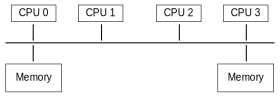
\includegraphics{memorder/SystemArchBus}}
\caption{Global System Bus And Multi-Copy Atomicity}
\label{fig:memorder:Global System Bus And Multi-Copy Atomicity}
\end{figure}

\emph{Multicopy atomic}~\cite{Stone:1995:SP:623262.623912} 플랫폼에서 돌아가는
쓰레드들은 스토어들의 순서에 대해서는 심지어 서로 다른 변수들에 대한 것조차도
동의를 할 것이 보장됩니다.
그런 시스템에 대한 유용한 상상의 모델은
Figure~\ref{fig:memorder:Global System Bus And Multi-Copy Atomicity}
에 보인 싱글 버스 아키텍쳐 같은 시스템입니다.
각각의 스토어가 버스로의 메세지를 낸다면, 그리고 이 버스가 한번에 하나의
스토어만 처리할 수 있다면, 모든 CPU 들은 모든 스토어에 대해 각각 관측한 순서가
동일할 겁니다.
불행히도, 그림에 보인 것처럼 스토어 버퍼나 캐시조차 없이 컴퓨터 시스템을
만드는건 빙하같은 계산속도가 나오게 할겁니다.
따라서 multicopy atomicity 를 제공하는데 흥미를 갖는 CPU 제조사들은 그대신 약간
더 완화된 \emph{other-multicopy atomicity}~\cite[Section B2.3]{ARMv8A:2017} 를
제공하고자 하게 되는데, 여기선 특정 스토어를 수행하는 CPU 는 모든 스토어들의
순서에 대한 CPU 들의 동의로부터 배제될 수 있게 해줍니다.
이는 CPU 들 중 일부만 스토어를 수행한다면, 다른 CPU 들은 스토어들의 순서에
동의함을 의미하는데, 따라서 ``other-multicopy atomicity'' 의 ``other'' 가
존재하는 겁니다.
Multicopy-atomic 플랫폼들과 달리, other-multicopy-atomic 플랫폼에서는, 스토어를
수행하는 CPU는 자신의 스토어를 더 빨리 관측할 수 있어서, 나중의 로드가 새로
스토어된 값을 스토어 버퍼로부터 곧바로 얻어올 수 있음을 의미합니다.
이는 끔찍한 플랫폼은 피할 수 있게 해줍니다.
\iffalse

Threads running on a \emph{multicopy atomic}~\cite{Stone:1995:SP:623262.623912}
platform are guaranteed
to agree on the order of stores, even to different variables.
A useful mental model of such a system is the single-bus architecture
shown in
Figure~\ref{fig:memorder:Global System Bus And Multi-Copy Atomicity}.
If each store resulted in a message on the bus, and if the bus could
accommodate only one store at a time, then any pair of CPUs would
agree on the order of all stores that they observed.
Unfortunately, building a computer system as shown in the figure,
without store buffers or even caches, would result in glacial computation.
CPU vendors interested in providing multicopy atomicity have therefore
instead provided the slightly weaker
\emph{other-multicopy atomicity}~\cite[Section B2.3]{ARMv8A:2017},
which excludes the CPU doing a given store from the requirement that all
CPUs agree on the order of all stores.
This means that if only a subset of CPUs are doing stores, the
other CPUs will agree on the order of stores, hence the ``other''
in ``other-multicopy atomicity''.
Unlike multicopy-atomic platforms, within other-multicopy-atomic platforms,
the CPU doing the store is permitted to observe its
store early, which allows its later loads to obtain the newly stored
value directly from the store buffer.
This in turn avoids abysmal performance.
\fi

\QuickQuiz{}
	Multicopy atomic 와 다른 multicopy atomic 사이의 다른 동작에 대한
	특정한 예를 들어볼 수 있겠습니까?
	\iffalse

	Can you give a specific example showing different behavior for
	multicopy atomic on the one hand and other-multicopy atomic
	on the other?
	\fi
\QuickQuizAnswer{
\begin{listing}[tbp]
{ \scriptsize
\begin{verbbox}[\LstLineNo]
C C-MP-OMCA+o-o-o+o-rmb-o

{
}

P0(int *x, int *y)
{
  int r0;

  WRITE_ONCE(*x, 1);
  r0 = READ_ONCE(*x);
  WRITE_ONCE(*y, r0);
}

P1(int *x, int *y)
{
  int r1;
  int r2;

  r1 = READ_ONCE(*y);
  smp_rmb();
  r2 = READ_ONCE(*x);
}

exists (1:r1=1 /\ 1:r2=0)
\end{verbbox}
}
\centering
\theverbbox
\caption{Litmus Test Distinguishing Multicopy Atomic From Other Multicopy Atomic}
\label{lst:memorder:Litmus Test Distinguishing Multicopy Atomic From Other Multicopy Atomic}
\end{listing}

	Listing~\ref{lst:memorder:Litmus Test Distinguishing Multicopy Atomic From Other Multicopy Atomic}
	(\path{C-MP-OMCA+o-o-o+o-rmb-o.litmus})
	이 그런 테스트를 보입니다.

	Multicopy-atomic 플랫폼에서, \co{P0()} 의 line~10 에서의 \co{x} 로의
	스토어는\co{P0()} 와 \co{P1()} 에게 동시에 보여야만 합니다.
	이 스토어는 \co{P0()} 에게 line~11 에서야 보이게 되고, line~12 에서의
	\co{P0()} 의 \co{y} 로의 스토어 전에, \co{P0()} 의 \co{x} 로의 스토어는
	\co{P1()} 을 포함해서 \co{y} 로의 스토어 전에 보여야만 합니다.
	따라서, line~20 에서 \co{P1()} 의 \co{y} 로부터의 로드가 값 1을
	리턴하면, line~21 에서의 \co{smp_rmb()} 가 이 두 로드의 수행 순서를
	강제하므로, line~22 에서의 \co{x} 역시 그래야만 합니다.
	따라서, line~25 의 \co{exists} 절은 multicopy-atomic 플랫폼에선느
	발동되지 않습니다.

	반면, other-multicopy-atomic 플랫폼에서는 \co{P0()} 가 자신의 스토어를
	일찍 볼 수 있으므로, \co{P1()} 이 이 두개의 스토어를 보는 순서에
	대해서는 제약이 없어서 \co{exists} 절이 발동될 수 있을 겁니다.
	\iffalse

	Listing~\ref{lst:memorder:Litmus Test Distinguishing Multicopy Atomic From Other Multicopy Atomic}
	(\path{C-MP-OMCA+o-o-o+o-rmb-o.litmus})
	shows such a test.

	On a multicopy-atomic platform, \co{P0()}'s store to \co{x} on
	line~10 must become visible to both \co{P0()} and \co{P1()}
	simultaneously.
	Because this store becomes visible to \co{P0()} on line~11, before
	\co{P0()}'s store to \co{y} on line~12, \co{P0()}'s store to
	\co{x} must become visible before its store to \co{y} everywhere,
	including \co{P1()}.
	Therefore, if \co{P1()}'s load from \co{y} on line~20 returns the
	value 1, so must its load from \co{x} on line~22, given that
	the \co{smp_rmb()} on line~21 forces these two loads to execute
	in order.
	Therefore, the \co{exists} clause on line~25 cannot trigger on a
	multicopy-atomic platform.

	In contrast, on an other-multicopy-atomic platform, \co{P0()}
	could see its own store early, so that there would be no constraint
	on the order of visibility of the two stores from to \co{P1()},
	which in turn allows the \co{exists} clause to trigger.
	\fi
} \QuickQuizEnd

모든 플랫폼이 어떤 형태의 multi-copy atomicity 를 제공하는 시대가 올수도
있겠습니다만, 그 사이에는 multicopy-atomic 이 아닌 플랫폼이 존재할 것이고,
따라서 소프트웨어는 그걸 잘 다뤄야 합니다.
\iffalse

Perhaps there will come a day when all platforms provide some flavor
of multi-copy atomicity, but
in the meantime, non-multicopy-atomic platforms do exist, and so software
does need to deal with them.
\fi

\begin{listing}[tbp]
{ \scriptsize
\begin{verbbox}[\LstLineNo]
C C-WRC+o+o-data-o+o-rmb-o

{
}

P0(int *x)
{
  WRITE_ONCE(*x, 1);
}

P1(int *x, int* y)
{
  int r1;

  r1 = READ_ONCE(*x);
  WRITE_ONCE(*y, r1);
}

P2(int *x, int* y)
{
  int r2;
  int r3;

  r2 = READ_ONCE(*y);
  smp_rmb();
  r3 = READ_ONCE(*x);
}

exists (1:r1=1 /\ 2:r2=1 /\ 2:r3=0)
\end{verbbox}
}
\centering
\theverbbox
\caption{WRC Litmus Test With Dependencies (No Ordering)}
\label{lst:memorder:WRC Litmus Test With Dependencies (No Ordering)}
\end{listing}

Listing~\ref{lst:memorder:WRC Litmus Test With Dependencies (No Ordering)}
(\path{C-WRC+o+o-data-o+o-rmb-o.litmus})
은 multicopy atomicity 를 보이고 있는데, multicopy-atomic 플랫폼 위에서라면
line~29 의 \co{exists} 절은 발동될 수 없습니다.
반면에, multicopy-atomic 이 아닌 플랫폼에서 이 \co{exists} 절은 \co{P1()} 의
액세스들은 data dependency 로 순서잡혀지고 \co{P2()} 의 액세스들은
\co{smp_rmb()} 로 순서잡혀짐에도 발동될 수 있습니다.
Multicopy atomicity 의 정의는 모든 쓰레드가 스토어의 순서에 동의할 것을, 즉
모든 스토어가 모든 쓰레드에 같은 시간에 도착하는 것으로 생각될 수도 있을 것을
요구함을 다시 이야기 드립니다.
따라서, multicopy-atomic 이 아닌 플랫폼은 다른 쓰레드에 다른 시간에 도착하는
스토어가 있을 수 있습니다.
특히, \co{P0()} 의 스토어는 \co{P2()} 에 도착하기 훨씬 전에 \co{P1()} 에 도착할
수도 있는데, 이는 \co{P1()} 의 스토어가 \co{P0()} 의 스토어보다 먼저 \co{P2()}
에 도착할 확률을 높입니다.
\iffalse

Listing~\ref{lst:memorder:WRC Litmus Test With Dependencies (No Ordering)}
(\path{C-WRC+o+o-data-o+o-rmb-o.litmus})
demonstrates multicopy atomicity, that is, on a multicopy-atomic platform,
the \co{exists} clause on line~29 cannot trigger.
In contrast, on a non-multicopy-atomic
platform this \co{exists} clause can trigger, despite
\co{P1()}'s accesses being ordered by a data dependency and \co{P2()}'s
accesses being ordered by an \co{smp_rmb()}.
Recall that the definition of multicopy atomicity requires that all
threads agree on the order of stores, which can be thought of as
all stores reaching all threads at the same time.
Therefore, a non-multicopy-atomic platform can have a store reach
different threads at different times.
In particular, \co{P0()}'s store might reach \co{P1()} long before it
reaches \co{P2()}, which raises the possibility that \co{P1()}'s store
might reach \co{P2()} before \co{P0()}'s store does.
\fi

\begin{figure}[tb]
\centering
\resizebox{3.0in}{!}{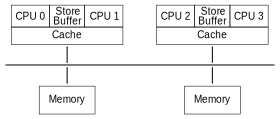
\includegraphics{memorder/NonMCAplatform}}
\caption{Shared Store Buffers And Multi-Copy Atomicity}
\label{fig:memorder:Shared Store Buffers And Multi-Copy Atomicity}
\end{figure}

이는 왜 일반적인 물리 법칙의 제한을 받는 실제 시스템이
Listing~\ref{lst:memorder:WRC Litmus Test With Dependencies (No Ordering)}
의 \co{exists} 절을 발동시키는지에 대한 의문을 낳습니다.
그런 실제 시스템에 대한 그림이
Figure~\ref{fig:memorder:Shared Store Buffers And Multi-Copy Atomicity} 에
그려져 있습니다.
CPU~0 와 CPU~1 은 스토어 버퍼를 공유하며, CPU~2 와~3 도 그렇습니다.
이는 CPU~1 은 이 스토어 버퍼로부터 값을 로드할 수 있으며, 따라서 CPU~0 가
스토어한 값을 곧바로 볼 가능성이 있습니다.
반면에, CPU~2 와~3 은 연관된 캐시 라인이 새로운 값을 자신에게 가져올 때까지
기다려야 합니다.
\iffalse

This leads to the question of why a real system constrained by the
usual laws of physics would ever trigger the \co{exists} clause of
Listing~\ref{lst:memorder:WRC Litmus Test With Dependencies (No Ordering)}.
The cartoonish diagram of a such a real system is shown in
Figure~\ref{fig:memorder:Shared Store Buffers And Multi-Copy Atomicity}.
CPU~0 and CPU~1 share a store buffer, as do CPUs~2 and~3.
This means that CPU~1 can load a value out of the store buffer, thus
potentially immediately seeing a value stored by CPU~0.
In contrast, CPUs~2 and~3 will have to wait for the corresponding cache
line to carry this new value to them.
\fi

\QuickQuiz{}
	대체 누가 공유된 스토어 버퍼를 갖는 시스템을 설계할 \emph{생각} 따위를
	하겠어요???
	\iffalse

	Then who would even \emph{think} of designing a system with shared
	store buffers???
	\fi
\QuickQuizAnswer{
	이는 코어당 여러 하드웨어 쓰레드를 갖는 시스템에서는 매우 자연스러운
	설계입니다.
	하드웨어의 관점에서는 자연스럽습니다, 이게요!
	\iffalse

	This is in fact a very natural design for any system having
	multiple hardware threads per core.
	Natural from a hardware point of view, that is!
	\fi
} \QuickQuizEnd

\begin{table*}[tbh]
\small
\centering\OneColumnHSpace{-0.8in}
\renewcommand*{\arraystretch}{1.1}
\rowcolors{13}{lightgray}{}
\begin{tabular}{rlllllll}\toprule
	& \multicolumn{1}{c}{\tco{P0()}} & \multicolumn{2}{c}{\tco{P0()} \& \tco{P1()}} &
		\multicolumn{1}{c}{\tco{P1()}} & \multicolumn{3}{c}{\tco{P2()}} \\
	\cmidrule(l){2-2} \cmidrule(l){3-4} \cmidrule(lr){5-5} \cmidrule(l){6-8}
	& Instruction & Store Buffer & Cache & Instruction &
			Instruction & Store Buffer & Cache \\
	\cmidrule{1-1} \cmidrule(l){2-2} \cmidrule(l){3-3} \cmidrule(l){4-4}
		\cmidrule(lr){5-5} \cmidrule(l){6-6} \cmidrule(l){7-7} \cmidrule(l){8-8}
	1 & (Initial state) & & \tco{y==0} &
		(Initial state) &
			(Initial state) & & \tco{x==0} \\
	2 & \tco{x = 1;} & \tco{x==1} & \tco{y==0} &
		 & & & \tco{x==0} \\
	3 & (Read-Invalidate \tco{x}) & \tco{x==1} & \tco{y==0} & \tco{r1 = x} (1)
		 & & & \tco{x==0} \\
	4 &  & \tco{x==1} \tco{y==1} & \tco{y==0} & \tco{y = r1}
		 & \tco{r2 = y} & & \tco{x==0} \\
	5 &  & \tco{x==1} & \tco{y==1} & (Finish store)
		 & (Read \tco{y}) & & \tco{x==0} \\
	6 & (Respond \tco{y}) & \tco{x==1} & \tco{y==1} &
		 & (\tco{r2==1}) & & \tco{x==0} \tco{y==1} \\
	7 & & \tco{x==1} & \tco{y==1} &
		 & \tco{smp_rmb()} & & \tco{x==0} \tco{y==1} \\
	8 & & \tco{x==1} & \tco{y==1} &
		 & \tco{r3 = x (0)} & & \tco{x==0} \tco{y==1} \\
	9 & & \tco{x==1} & \tco{x==0} \tco{y==1} &
		 & (Respond \tco{x}) & & \tco{y==1} \\
	10 & (Finish store) & & \tco{x==1} \tco{y==1} &
		 &  & & \tco{y==1} \\
	\bottomrule
\end{tabular}
\caption{Memory Ordering: WRC Sequence of Events}
\label{tab:memorder:Memory Ordering: WRC Sequence of Events}
\end{table*}

Table~\ref{tab:memorder:Memory Ordering: WRC Sequence of Events}
은
Listing~\ref{lst:memorder:WRC Litmus Test With Dependencies (No Ordering)}
의 \co{exists} 절이 발동될 수 있는 일련의 이벤트를 보입니다.
이 일련의 이벤트는 \co{P0()} 와 \co{P1()} 이
Figure~\ref{fig:memorder:Shared Store Buffers And Multi-Copy Atomicity} 에 보인
방식으로 캐시와 스토어 버퍼를 공유한다는 점에 상당히 의존적입니다.
\iffalse

Table~\ref{tab:memorder:Memory Ordering: WRC Sequence of Events}
shows one sequence of events that can result in the \co{exists} clause in
Listing~\ref{lst:memorder:WRC Litmus Test With Dependencies (No Ordering)}
triggering.
This sequence of events will depend critically on \co{P0()} and
\co{P1()} sharing both cache and a store buffer in the manner shown in
Figure~\ref{fig:memorder:Shared Store Buffers And Multi-Copy Atomicity}.
\fi

\QuickQuiz{}
	하지만 \co{P0()} 와 \co{P1()} 은 스토어 버퍼와 캐시를 공유해야 하는데
	\co{P2()} 는 자기만의 캐시와 스토어 버퍼를 갖는다는게 공평한가요???
	\iffalse

	But just how is it fair that \co{P0()} and \co{P1()} must share a store
	buffer and a cache, but \co{P2()} gets one each of its very own???
	\fi
\QuickQuizAnswer{
	어쩌면
	Figure~\ref{fig:memorder:Shared Store Buffers And Multi-Copy Atomicity}
	에 보인 것처럼 \co{P3()} 가 존재해서 \co{P2()} 의 스토어 버퍼와 캐시를
	공유할 수도 있을 겁니다.  하지만 꼭 그래야 하는 건 아니죠.
	일부 플랫폼은 서로 다른 코어들이 서로 다른 수의 쓰레드들을 불능화
	시키는걸 가능하게 해서, 하드웨어가 당장 처리해야할 워크로드의 필요에
	맞게 조정될 수 있게 합니다.
	예를 들어, 워크로드의 싱글 쓰레드로 돌아가는 중요한 지점은 하나의
	쓰레드만 돌아갈 수 있는 코어에 할당되어서 이 워크로드의 해당 부분을 이
	하나의 쓰레드가 해당 코어의 모든 가능한 자원을 사용할 수 있게 할 수
	있을 겁니다.
	워크로드의 더 높은 병렬성을 갖지만 캐시미스에 취약한 부분은 더 나은
	처리량을 제공하기 위해 모든 하드웨어 쓰레드를 사용할 수 있는 코어들에
	할당될 수 있을 겁니다.
	이렇게 향상된 처리량은 하나의 하드웨어 쓰레드가 캐시 미스에 의해 멈춰
	있는 동안, 다른 하드웨어 쓰레드는 진행을 이룰 수 있기 때문이기도
	할겁니다.

	이런 경우, 성능 요구사항은 독특한 사람의 관점에서의 공평성보다
	우선합니다.
	\iffalse

	Presumably there is a \co{P3()}, as is in fact shown in
	Figure~\ref{fig:memorder:Shared Store Buffers And Multi-Copy Atomicity},
	that shares \co{P2()}'s store buffer and cache.
	But not necessarily.
	Some platforms allow different cores to disable different numbers
	of threads, allowing the hardware to adjust to the needs of the
	workload at hand.
	For example, a single-threaded critical-path portion of the workload
	might be assigned to a core with only one thread enabled, thus
	allowing the single thread running that portion of the workload
	to use the entire capabilities of that core.
	Other more highly parallel but cache-miss-prone portions of the
	workload might be assigned to cores with all hardware threads
	enabled to provide improved throughput.
	This improved throughput could be due to the fact that while one
	hardware thread is stalled on a cache miss, the other hardware
	threads can make forward progress.

	In such cases, performance requirements override quaint human
	notions of fairness.
	\fi
} \QuickQuizEnd

Row~1 은 최초의 상태를 보이는데, \co{y} 는 \co{P0()} 와 \co{P1()} 의 공유된
캐시에, \co{x} 의 최초 값은 \co{P2()} 의 캐시에 있습니다.

Row~2 는 \co{P0()} 의 line~8 에서의 스토어가 수행된 직후의 효과를 보입니다.
\co{x} 를 담고 있는 캐시라인은 \co{P0()} 와 \co{P1()} 의 공유 캐시에 있지
않으므로, 새로운 값 (\co{1}) 은 해당 CPU 들의 공유 스토어 버퍼에 저장됩니다.

Row~3 는 두개의 사건을 보입니다.
먼저, \co{P0()} 는 \co{x} 의 새로운 값을 공유 스토어 버퍼에서 내려보낼 수
있게끔 \co{x} 를 담고 있는 캐시라인을 얻어오기 위해 read-invalidate
오퍼레이션을 날립니다.
이어서, \co{P1()} 은 \co{x} 를 읽어오는데 (line~15), 이 오퍼레이션은 \co{x} 의
새로운 값을 공유 스토어 버퍼에서 곧바로 얻어올 수 있기 때문에 즉각적으로
완료됩니다.
\iffalse

Row~1 shows the initial state, with the initial value of \co{y} in
\co{P0()}'s and \co{P1()}'s shared cache, and the initial value of \co{x} in
\co{P2()}'s cache.

Row~2 shows the immediate effect of \co{P0()} executing its store on line~8.
Because the cacheline containing \co{x} is not in \co{P0()}'s and \co{P1()}'s
shared cache, the new value (\co{1}) is stored in the shared store buffer.

Row~3 shows two transitions.
First, \co{P0()} issues a read-invalidate operation to fetch the cacheline
containing \co{x} so that it can flush the new value for \co{x} out of
the shared store buffer.
Second, \co{P1()} loads from \co{x} (line~15), an operation that completes
immediately because the new value of \co{x} is immediately available
from the shared store buffer.
\fi

Row~4 또한 두개의 사건을 보입니다.
먼저, \co{P1()} 이 \co{y} 로의 스토어 (line~16) 을 수행한 직후의 효과로, 이
새로운 값은 공유 스토어 버퍼에 저장됨을 보입니다.
이어서, \co{P2()} 의 \co{y} 로부터의 로드 (line~24) 를 보입니다.

Row~5 는 두개의 사건의 이후 흐름을 보입니다.
먼저, \co{P1()} 은 \co{y} 로의 스토어를 완료하고, 공유 스토어 버퍼에서 캐시로
값을 내림을 보입니다.
또한, \co{P2()} 의 \co{y} 를 담고 있는 캐시라인으로의 요청을 보입니다.

Row~6 는 \co{P2()} 가 \co{y} 를 담고 있는 캐시라인을 받아서 \co{r2} 로의 로드를
마칠 수 있게 해주는데, 이 로드는 \co{1} 의 값을 가져오게 됩니다.

Row~7 은 \co{P2()} 가 \co{smp_rmb()} 를 수행해서 (line~25), 두 로드의 순서를
강제하는 것을 보입니다.
\iffalse

Row~4 also shows two transitions.
First, it shows the immediate effect of \co{P1()} executing its store to
\co{y} (line~16), placing the new value into the shared store buffer.
Second, it shows the start of \co{P2()}'s load from \co{y} (line~24).

Row~5 continues the tradition of showing two transitions.
First, it shows \co{P1()} complete its store to \co{y}, flushing
from the shared store buffer to the cache.
Second, it shows \co{P2()} request the cacheline containing \co{y}.

Row~6 shows \co{P2()} receive the cacheline containing \co{y}, allowing
it to finish its load into \co{r2}, which takes on the value \co{1}.

Row~7 shows \co{P2()} execute its \co{smp_rmb()} (line~25), thus keeping
its two loads ordered.
\fi

Row~8 은 \co{P2()} 가 \co{x} 로부터의 로드를 수행하는 것을 보이는데, 이는
\co{P2()} 의 캐시로부터 값 0을 곧바로 가져올 겁니다

Row~9 은 \emph{마침내} \co{P2()} 가 \co{P0()} 의, row~3 에서 보내졌던, \co{x}
를 담고 있는 캐시라인에 대한 요청에 응답하게 되는 것을 보입니다.

마지막으로, row~10 은 \co{P0()} 가 자신의 스토어를 끝내서, \co{x} 에 대한 값을
자신의 공유 스토어 버퍼에서 공유된 캐시로 내리는 것을 보입니다.

Line~29 의 \co{exists} 절이 발동됨 역시 알아두시기 바랍니다.
\co{r1} 과 \co{r2} 의 값들은 모두 값 1을 갖고, \co{r3} 의 마지막 값은 값
0입니다.
이 이상한 결과는 \co{P0()} 의 \co{x} 에 대한 새로운 값이 \co{P2()} 와 이야기
하기 전에 \co{P1()} 에게 전달되었기 때문에 발생했습니다.
\iffalse

Row~8 shows \co{P2()} execute its load from \co{x}, which immediately
returns with the value zero from \co{P2()}'s cache.

Row~9 shows \co{P2()} \emph{finally} responding to \co{P0()}'s request for
the cacheline containing \co{x}, which was made way back up on row~3.

Finally, row~10 shows \co{P0()} finish its store, flushing its value of
\co{x} from the shared store buffer to the shared cache.

Note well that the \co{exists} clause on line~29 has triggered.
The values of \co{r1} and \co{r2} are both the value one, and
the final value of \co{r3} the value zero.
This strange result occurred because \co{P0()}'s new value of \co{x} was
communicated to \co{P1()} long before it was communicated to \co{P2()}.
\fi

\QuickQuiz{}
	Table~\ref{tab:memorder:Memory Ordering: WRC Sequence of Events}
	대로라면, \co{P1()} 의 스토어는 그렇게 빨리 끝나는데 \co{P0()} 의
	스토어는 왜 그렇게 오래 걸리나요?
	달리 말하자면,
	Listing~\ref{lst:memorder:WRC Litmus Test With Dependencies (No Ordering)}
	의 line~32 에 있는 \co{exists} 절은 정말로 실제 시스템에서도
	발동되는건가요?
	\iffalse

	Referring to
	Table~\ref{tab:memorder:Memory Ordering: WRC Sequence of Events},
	why on earth would \co{P0()}'s store take so long to complete when
	\co{P1()}'s store complete so quickly?
	In other words, does the \co{exists} clause on line~32 of
	Listing~\ref{lst:memorder:WRC Litmus Test With Dependencies (No Ordering)}
	really trigger on real systems?
	\fi
\QuickQuizAnswer{
	정말로 발동될 수 있다는 사실을 받아들여야 합니다.
	Akira Yokosawa 는 \co{litmus7} 이라는 도구를 사용해 \Power{8}
	시스템에서 이 리트머스 테스트를 돌려봤습니다.
	1,000,000,000 번의 시도 중에, 4 번 \co{exists} 절이
	발동되었습니다.
	따라서, \co{exists} 절의 발동 확률은 백만번에 한번도 아니고, 일억번 중
	한번입니다.
	하지만 실제 시스템에서도 발동된다는 것은 사실입니다.
	\iffalse

	You need to face the fact that it really can trigger.
	Akira Yokosawa used the \co{litmus7} tool to run this litmus test
	on a \Power{8} system.
	Out of 1,000,000,000 runs, 4 triggered the \co{exists} clause.
	Thus, triggering the \co{exists} clause is not merely a one-in-a-million
	occurrence, but rather a one-in-a-hundred-million occurrence.
	But it nevertheless really does trigger on real systems.
	\fi
} \QuickQuizEnd

의존성이 순서를 제공하긴 하지만, 각자의 쓰레드 스스로에 대해서만 제공하기
때문에 이 반직관적인 결과가 일어납니다.
이 세개 쓰레드 예제는 더 강한 순서 규칙을 필요로 하는데,
Section~\ref{sec:memorder:Cumulativity}
부터~\ref{sec:memorder:Release-Acquire Chains} 까지의 주제가 이를 다룹니다.
\iffalse

This counter-intuitive result happens because although dependencies
do provide ordering, they provide it only within the confines of their
own thread.
This three-thread example requires stronger ordering, which
is the subject of
Sections~\ref{sec:memorder:Cumulativity}
through~\ref{sec:memorder:Release-Acquire Chains}.
\fi

\subsubsection{Cumulativity}
\label{sec:memorder:Cumulativity}

Listing~\ref{lst:memorder:WRC Litmus Test With Dependencies (No Ordering)}
에 보인 세개 쓰레드의 예제는 \emph{cumulative} 순서 규칙, 또는
\emph{cumulativity} 라 불리는 순서 규칙을 필요로 합니다.
Cumulative 메모리 순서 강제 오퍼레이션은 그 앞의 액세스들만이 아니라 같은
변수에 대한 모든 쓰레드의 이전 액세스들까지 순서를 강제해줍니다.
\iffalse

The three-thread example shown in
Listing~\ref{lst:memorder:WRC Litmus Test With Dependencies (No Ordering)}
requires \emph{cumulative} ordering, or \emph{cumulativity}.
A cumulative memory-ordering operation orders not just any given
access preceding it, but also earlier accesses by any thread to that
same variable.
\fi

\begin{listing}[tbp]
{ \scriptsize
\begin{verbbox}[\LstLineNo]
C C-WRC+o+o-r+a-o

{
}

P0(int *x)
{
  WRITE_ONCE(*x, 1);
}

P1(int *x, int* y)
{
  int r1;

  r1 = READ_ONCE(*x);
  smp_store_release(y, r1);
}

P2(int *x, int* y)
{
  int r2;
  int r3;

  r2 = smp_load_acquire(y);
  r3 = READ_ONCE(*x);
}

exists (1:r1=1 /\ 2:r2=1 /\ 2:r3=0)
\end{verbbox}
}
\centering
\theverbbox
\caption{WRC Litmus Test With Release}
\label{lst:memorder:WRC Litmus Test With Release}
\end{listing}

의존성은 cumulativity 를 제공하지 않는데,
Table~\ref{tab:memorder:Linux-Kernel Memory-Ordering Cheat Sheet} 의
\co{smp_read_barrier_depends()} 와 \co{READ_ONCE()} 행이 모두 ``C'' 열을 비워둔
이유입니다.
하지만, release 오퍼레이션들은 ``C'' 열의 ``C'' 가 알리듯이, cumulativity 를
제공합니다.
따라서,
Listing~\ref{lst:memorder:WRC Litmus Test With Release}
(\path{C-WWC+o+o-r+o-addr-o.litmus})
은
Listing~\ref{lst:memorder:WRC Litmus Test With Dependencies (No Ordering)}
의 data dependency 를 위한 release 오퍼러이션을 대체합니다.
Release 오퍼레이션은 cumulative 하기 때문에, 그 순서 강제는
Listing~\ref{lst:memorder:WRC Litmus Test With Release} 의 line~15 에서의
\co{P1()} 에 의한 \co{x} 로부터의 로드만이 아니라 line~8 의 \co{P0()} 에 의한
\co{x} 로의 스토어에도 적용됩니다---하지만 그 로드가 스토어된 값을 리턴할
경우만으로, line~28 의 \co{exists} 절 안의 \co{1:r1=1} 이 맞을 경우만
그렇습니다.
이는 \co{P2()} 의 load-acquire 는 line~25 에서의 \co{x} 로부터의 로드가 line~8
의 스토어 뒤에 일어난 것으로 강제하기 충분해서, 리턴되는 값은 1로, \co{2:r3=0}
는 맞지 않게 되어서, 결국 \co{exists} 절이 발동되지 않게 함을 의미합니다.
\iffalse

Dependencies do not provide cumulativity,
which is why the ``C'' column is blank for
both the \co{READ_ONCE()} and the \co{smp_read_barrier_depends()} rows
of Table~\ref{tab:memorder:Linux-Kernel Memory-Ordering Cheat Sheet}.
However, as indicated by the ``C'' in their ``C'' column,
release operations do provide cumulativity.
Therefore,
Listing~\ref{lst:memorder:WRC Litmus Test With Release}
(\path{C-WRC+o+o-r+a-o.litmus})
substitutes a release operation for
Listing~\ref{lst:memorder:WRC Litmus Test With Dependencies (No Ordering)}'s
data dependency.
Because the release operation is cumulative, its ordering applies not only to
Listing~\ref{lst:memorder:WRC Litmus Test With Release}'s
load from \co{x} by \co{P1()} on line~15, but also to the store to \co{x}
by \co{P0()} on line~8---but only if that load returns the value stored,
which matches the \co{1:r1=1} in the \co{exists} clause on line~28.
This means that \co{P2()}'s load-acquire suffices to force the
load from \co{x} on line~25 to happen after the store on line~8, so
the value returned is one, which does not match \co{2:r3=0}, which
in turn prevents the \co{exists} clause from triggering.
\fi

\begin{figure*}[htbp]
\centering
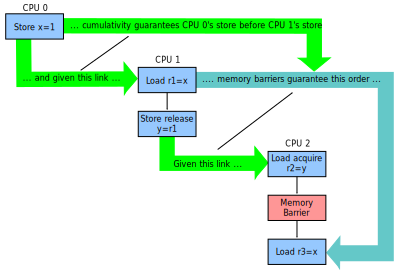
\includegraphics{memorder/memorybarriercum}
\caption{Cumulativity}
\label{fig:memorder:Cumulativity}
\end{figure*}

이런 순서 규칙은
Figure~\ref{fig:memorder:Cumulativity} 에 그려져 있습니다.
Cumulativity 는 한단계 이전의 시간으로만 제한되는게 아님을 알아두시기 바랍니다.
어떤 쓰레드에서건 line~13 에서의 스토어 전에 \co{x} 로의 스토어 또는 \co{x}
로부터의 로드가 있었다면, \co{r1} 과 \co{r2} 가 모두 \co{x} 의 주소를 갖게 되는
경우에 한해서이긴 하지만 그 앞의 로드나 스토어 역시 line~32 에서의 스토어
전으로 순서잡히게 됩니다.

정리해보면, cumulative 순서 강제 오퍼레이션의 사용은 일부 상황에서의
non-multicopy-atomic 동작을 막을 수 있습니다.
그렇다고 해도 Cumulativity 는 한계가 있는데, 이에 대해 다음 섹션에서
알아봅니다.
\iffalse

These ordering constraints are depicted graphically in
Figure~\ref{fig:memorder:Cumulativity}.
Note also that cumulativity is not limited to a single step back in time.
If there was another load from \co{x} or store to \co{x} from any thread
that came before the store on line~13, that prior load or store would also
be ordered before the store on line~32, though only if both \co{r1} and
\co{r2} both end up containing the address of \co{x}.

In short, use of cumulative ordering operations can suppress
non-multicopy-atomic behaviors in some situations.
Cumulativity nevertheless has limits, which are examined in the next section.
\fi

\subsubsection{Propagation}
\label{sec:memorder:Propagation}

\begin{listing}[tbp]
{ \scriptsize
\begin{verbbox}[\LstLineNo]
C C-W+RWC+o-r+a-o+o-mb-o

{
int x = 0;
int y = 0;
int z = 0;
}

P0(int *x, int *y)
{
  WRITE_ONCE(*x, 1);
  smp_store_release(y, 1);
}

P1(int *y, int *z)
{
  int r1;
  int r2;

  r1 = smp_load_acquire(y);
  r2 = READ_ONCE(*z);
}

P2(int *z, int *x)
{
  int r3;

  WRITE_ONCE(*z, 1);
  smp_mb();
  r3 = READ_ONCE(*x);
}

exists(1:r1=1 /\ 1:r2=0 /\ 2:r3=0)
\end{verbbox}
}
\centering
\theverbbox
\caption{W+RWC Litmus Test With Release (No Ordering)}
\label{lst:memorder:W+RWC Litmus Test With Release (No Ordering)}
\end{listing}

Listing~\ref{lst:memorder:W+RWC Litmus Test With Release (No Ordering)}
(\path{C-W+RWC+o-r+a-o+o-mb-o.litmus})
은 cumulativity 와 store-release 가 전체 메모리 배리어의 도움에도 불구하고 갖는
한계를 보입니다.
문제는, line~12 에서의 \co{smp_store_release()} 가 cumulativity 를 가짐에도
불구하고, 그리고 이 cumulativity 가 line~30 에서의 \co{P2()} 의 로드를
순서잡음에도 불구하고, \co{smp_store_release()} 의 순서규칙은 \co{P1()} 의 로드
(line~21) 와 \co{P2()} 의 스토어 (line~28) 에 전파될 수 없다는 것입니다.
이는 line~33 에서의 \co{exitst} 절이 발동될 수 있음을 의미합니다.
\iffalse

Listing~\ref{lst:memorder:W+RWC Litmus Test With Release (No Ordering)}
(\path{C-W+RWC+o-r+a-o+o-mb-o.litmus})
shows the limitations of cumulativity and of store-release,
even with a full memory barrier helping out.
The problem is that although the \co{smp_store_release()} on
line~12 has cumulativity, and although that cumulativity does
order \co{P2()}'s load on line~30, the \co{smp_store_release()}'s
ordering cannot propagate through the combination of \co{P1()}'s
load (line~21) and \co{P2()}'s store (line~28).
This means that the \co{exists} clause on line~33 really can trigger.
\fi

\QuickQuiz{}
	하지만 이 리트머스 테스트에 최소 세개의 쓰레드가 존재하지 않는다면
	전파에 대해서는 걱정할 필요가 없을 거예요, 그렇죠?
	\iffalse

	But it is not necessary to worry about propagation unless
	there are at least three threads in the litmus test, right?
	\fi
\QuickQuizAnswer{
\begin{listing}[tbp]
{ \scriptsize
\begin{verbbox}[\LstLineNo]
C C-R+o-wmb-o+o-mb-o
{
}

P0(int *x0, int *x1)
{
  WRITE_ONCE(*x0, 1);
  smp_wmb();
  WRITE_ONCE(*x1, 1);
}


P1(int *x0, int *x1)
{
  int r2;

  WRITE_ONCE(*x1, 2);
  smp_mb();
  r2 = READ_ONCE(*x0);
}

exists (1:r2=0 /\ x1=2)
\end{verbbox}
}
\centering
\theverbbox
\caption{R Litmus Test With Write Memory Barrier (No Ordering)}
\label{lst:memorder:R Litmus Test With Write Memory Barrier (No Ordering)}
\end{listing}
	그렇지 않습니다.

	Listing~\ref{lst:memorder:R Litmus Test With Write Memory Barrier (No Ordering)}
	(\path{C-R+o-wmb-o+o-mb-o.litmus})
	은 propagation 을 필요로 하는 두개 쓰레드의 리트머스 테스트를 보이는데,
	여기선 두 쓰레드 사이에 store-to-store 와 load-to-store 연결만이
	존재하기 때문입니다.
	\co{P0()} 가 \co{smp_wmb()} 를 통해 순서를 제대로 잡았고 \co{P1()} 이
	\co{smp_mb()} 를 통해 완전히 순서를 잡았지만, 이 연결들의 근본적인 반
	임시적 성격은 line~22 의 \co{exists} 절이 정말로 발동될 수 있음을
	의미합니다.
	이 발동을 막으려면, line~8 의 \co{smp_wmb()} 는 \co{smp_mb()} 가
	되어서, 각각의 임시적이지 않은 링크마다 한번씩, 전파가 두번 발생하게
	만들어야 합니다.
	\iffalse

	Wrong.

	Listing~\ref{lst:memorder:R Litmus Test With Write Memory Barrier (No Ordering)}
	(\path{C-R+o-wmb-o+o-mb-o.litmus})
	shows a two-thread litmus test that requires propagation due to
	the fact that it only has store-to-store and load-to-store
	links between its pair of threads.
	Even though \co{P0()} is fully ordered by the \co{smp_wmb()} and
	\co{P1()} is fully ordered by the \co{smp_mb()}, the
	counter-temporal nature of the links means that
	the \co{exists} clause on line~22 really can trigger.
	To prevent this triggering, the \co{smp_wmb()} on line~8
	must become an \co{smp_mb()}, bringing propagation into play
	twice, once for each non-temporal link.
	\fi
} \QuickQuizEnd

\begin{figure}[htbp]
\centering
\resizebox{\columnwidth}{!}{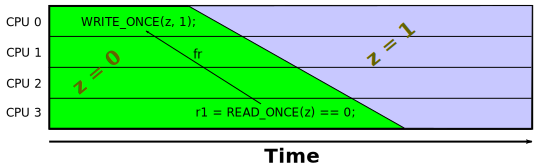
\includegraphics{memorder/fr}}
\caption{Load-to-Store is Counter-Temporal}
\label{fig:memorder:Load-to-Store is Counter-Temporal}
\end{figure}

이 상황은 완전히 반직관적으로 보일 수도 있겠습니다만, 빛의 속도는 제한되어 있고
컴퓨터는 크기가 존재함을 기억하시기 바랍니다.
따라서 \co{P2()} 의 \co{z} 로의 스토어가 \co{P1()} 에게 전달되기까지는
시간을필요로 하고, 이는 결국 \co{P1()} 의 \co{z} 로부터의 읽기가 시간상으로
훨씬 뒤에 일어날 수 있지만, 예전 값인 0을 읽을 수 있습니다.
이 상황은
Figure~\ref{fig:memorder:Load-to-Store is Counter-Temporal} 에 그려져 있습니다:
어떤 로드가 기존 값을 본다는 것은 이 로드가 새로운 값에 대한 스토어보다 먼저
수행되었음을 의미하지는 \emph{않습니다}.
\iffalse

This situation might seem completely counter-intuitive, but keep
in mind that the speed of light is finite and computers are of
non-zero size.
It therefore takes time for the effect of the \co{P2()}'s store to
\co{z} to propagate to \co{P1()}, which in turn means that it is possible
that \co{P1()}'s read from \co{z} happens much later in time, but
nevertheless still sees the old value of zero.
This situation is depicted in
Figure~\ref{fig:memorder:Load-to-Store is Counter-Temporal}:
Just because a load sees the old value does \emph{not} mean that
this load executed at an earlier time than did the store of the
new value.
\fi

Listing~\ref{lst:memorder:W+RWC Litmus Test With Release (No Ordering)}
또한, 두개가 아니라 세개의 프로세스가 있음으로 인해 메모리 배리어 짝 맞추기의
한계를 보이고 있음을 알아두시기 바랍니다.
이런 보다 복잡한 리트머스 테스트들은 \emph{사이클} 을 가지고 있다고 말할 수도
있는데, 메모리 배리어 짝 맞추기는 두개 쓰레드 사이클이 있는 특별한 경우입니다.
Listing~\ref{lst:memorder:W+RWC Litmus Test With Release (No Ordering)}
의 사이클은 \co{P0()} (line~11 과~12), \co{P1()} (line~20 과~21), \co{P2()}
(line~28, 29, 그리고~30), 그리고 다시 \co{P0()} (line~11) 로 이어집니다.
여기서의 \co{exists} 절은 이 사이클을 설명합니다:
\co{1:r1=1} 은 line~20 에서의 \co{smp_load_acquire()} 가 line~12 에서
\co{smp_store_release()} 가 저장한 값을 리턴했음을 의미하고, \co{1:r2=0} 는
line~28 에서의 \co{WRITE_ONCE()} 가 line~21 에서의 \co{READ_ONCE()} 에 의해
리턴되는 값에 영향을 끼치기에는 너무 늦게 도달했음을 의미하며, 마지막으로
\co{2:r3=0} 는 line~11 에서의 \co{WRITE_ONCE()} 가 line~30 에서의
\co{READ_ONCE()} 에 의해 리턴되는 값에 영향을 끼치기에는 너무 늦게 도착했음을
의미합니다.
이 경우, \co{exists} 절이 발동될 수 있다는 사실은 이 사이클이 \emph{허용된}
것이라고 이야기 됩니다.
반대로, \co{exists} 절이 발동될 수 없는 경우라면, 이 사이클이 \emph{금지된}
것이라고 이야기 됩니다.
\iffalse

Note that
Listing~\ref{lst:memorder:W+RWC Litmus Test With Release (No Ordering)}
also shows the limitations of memory-barrier pairing, given that
there are not two but three processes.
These more complex litmus tests can instead be said to have \emph{cycles},
where memory-barrier pairing is the special case of a two-thread cycle.
The cycle in
Listing~\ref{lst:memorder:W+RWC Litmus Test With Release (No Ordering)}
goes through \co{P0()} (lines~11 and~12), \co{P1()} (lines~20 and~21),
\co{P2()} (lines~28, 29, and~30), and back to \co{P0()} (line~11).
The \co{exists} clause delineates this cycle:
the \co{1:r1=1} indicates that the \co{smp_load_acquire()} on line~20
returned the value stored by the \co{smp_store_release()} on line~12,
the \co{1:r2=0} indicates that the \co{WRITE_ONCE()} on line~28 came
too late to affect the value returned by the \co{READ_ONCE()} on line~21,
and finally the \co{2:r3=0} indicates that the
\co{WRITE_ONCE()} on line~11 came too late to affect the value returned
by the \co{READ_ONCE()} on line~30.
In this case, the fact that the \co{exists} clause can trigger means that
the cycle is said to be \emph{allowed}.
In contrast, in cases where the \co{exists} clause cannot trigger,
the cycle is said to be \emph{prohibited}.
\fi

\begin{listing}[tbp]
{ \scriptsize
\begin{verbbox}[\LstLineNo]
C C-W+RWC+o-mb-o+a-o+o-mb-o

{
int x = 0;
int y = 0;
int z = 0;
}

P0(int *x, int *y)
{
  WRITE_ONCE(*x, 1);
  smp_mb();
  WRITE_ONCE(*y, 1);
}

P1(int *y, int *z)
{
  int r1;
  int r2;

  r1 = smp_load_acquire(y);
  r2 = READ_ONCE(*z);
}

P2(int *z, int *x)
{
  int r3;

  WRITE_ONCE(*z, 1);
  smp_mb();
  r3 = READ_ONCE(*x);
}

exists(1:r1=1 /\ 1:r2=0 /\ 2:r3=0)
\end{verbbox}
}
\centering
\theverbbox
\caption{W+WRC Litmus Test With More Barriers}
\label{lst:memorder:W+WRC Litmus Test With More Barriers}
\end{listing}

하지만 우리가
Listing~\ref{lst:memorder:W+RWC Litmus Test With Release (No Ordering)}
의 line~33 에 있는 \co{exists} 절을 유지해야 한다면 어떡해야 할까요?
한가지 해결책은 \co{P0()} 의 \co{smp_store_release()} 를
Table~\ref{tab:memorder:Linux-Kernel Memory-Ordering Cheat Sheet}
이 보이듯 cumulativity 만이 아니라 propagation 도 갖는
\co{smp_mb()} 로 교체하는 것입니다.
그렇게 한 결과가
Listing~\ref{lst:memorder:W+WRC Litmus Test With More Barriers}
(\path{C-W+RWC+o-mb-o+a-o+o-mb-o.litmus})
에 보여져 있습니다.
\iffalse

But what if we need to keep the \co{exists} clause on line~33 of
Listing~\ref{lst:memorder:W+RWC Litmus Test With Release (No Ordering)}?
One solution is to replace \co{P0()}'s \co{smp_store_release()}
with an \co{smp_mb()}, which
Table~\ref{tab:memorder:Linux-Kernel Memory-Ordering Cheat Sheet}
shows to have not only cumulativity, but also propagation.
The result is shown in
Listing~\ref{lst:memorder:W+WRC Litmus Test With More Barriers}
(\path{C-W+RWC+o-mb-o+a-o+o-mb-o.litmus}).
\fi

\QuickQuiz{}
	\co{smp_mb()} 가 propagation 속성을 갖는다면,
	Listing~\ref{lst:memorder:W+RWC Litmus Test With Release (No Ordering)}
	line~29 의 \co{smp_mb()} 는 왜 \co{exists} 절이 발동되는 걸 막지 못하는
	거죠?
	\iffalse

	But given that \co{smp_mb()} has the propagation property,
	why doesn't the \co{smp_mb()} on line~29 of
	Listing~\ref{lst:memorder:W+RWC Litmus Test With Release (No Ordering)}
	prevent the \co{exists} clause from triggering?
	\fi
\QuickQuizAnswer{
	대략적 경험상의 법칙으로는, \co{smp_mb()} 배리어의 propagation 속성은
	프로세스들 사이에 하나의 store-to-load 연결에 순서를 지키기에만
	충분합니다.
	불행히도,
	Listing~\ref{lst:memorder:W+RWC Litmus Test With Release (No Ordering)}
	는 한개가 아니라 두개의 store-to-load 연결을 가지고 있는데, 첫번째는
	line~21 에서의 \co{READ_ONCE()} 로부터 line~28 의 \co{WRITE_ONCE()}
	로의 것이고 두번째는 line~30 의 \co{READ_ONCE()} 로부터 line~11 의
	\co{WRITE_ONCE()} 로의 것입니다.
	따라서, \co{exists} 절이 발동되는 것을 막기 위해선 한개가 아니라 두개의
	\co{smp_mb()} 를 필요로 합니다.

	이 경험상의 법칙에 대한 특수한 예외로, 하나의 release-acquire 묶음은
	프로세스들 사이의 하나의 load-to-store 링크를 가질 수 있고, 여전히
	사이클을 금지합니다.
	\iffalse

	As a rough rule of thumb, the \co{smp_mb()} barrier's
	propagation property is sufficient to maintain ordering
	through only one store-to-load link between
	processes.
	Unfortunately,
	Listing~\ref{lst:memorder:W+RWC Litmus Test With Release (No Ordering)}
	has not one but two store-to-load links, with the
	first being from the \co{READ_ONCE()} on line~21 to the
	\co{WRITE_ONCE()} on line~28 and the second being from
	the \co{READ_ONCE()} on line~30 to the \co{WRITE_ONCE()}
	on line~11.
	Therefore, preventing the \co{exists} clause from triggering
	should be expected to require not one but two
	instances of \co{smp_mb()}.

	As a special exception to this rule of thumb, a release-acquire
	chain can have one load-to-store link between processes
	and still prohibit the cycle.
	\fi
} \QuickQuizEnd

\begin{figure}[tbp]
\centering
\resizebox{\columnwidth}{!}{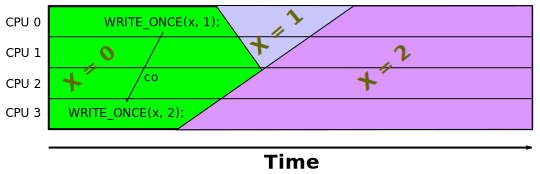
\includegraphics{memorder/co}}
\caption{Store-to-Store is Counter-Temporal}
\label{fig:memorder:Store-to-Store is Counter-Temporal}
\end{figure}

완전함을 기하기 위해,
Figure~\ref{fig:memorder:Store-to-Store is Counter-Temporal}
는 같은 변수를 향핸 여러 스토어들 가운데 ``승리하는'' 스토어는 가장 마지막에
행해진 스토어가 아닐 수 있음을 보이고 있습니다.
Figure~\ref{fig:memorder:A Variable With More Simultaneous Values} 를 주의깊게
이해한 사람에게 이는 그다지 놀라운 일이 아닐 겁니다.

하지만 가끔 시간은 우리 편이기도 한데, 다음 섹션에서 이를 보이겠습니다.
\iffalse

For completeness,
Figure~\ref{fig:memorder:Store-to-Store is Counter-Temporal}
shows that the ``winning'' store among a group of stores to the
same variable is not necessarily the store that started last.
This should not come as a surprise to anyone who carefully examined
Figure~\ref{fig:memorder:A Variable With More Simultaneous Values}.

But sometimes time is on our side, as shown in the next section.
\fi

\subsubsection{Happens-Before}
\label{sec:memorder:Happens-Before}

\begin{figure}[tbp]
\centering
\resizebox{\columnwidth}{!}{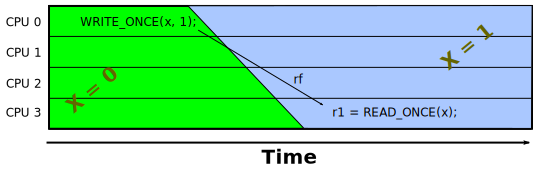
\includegraphics{memorder/rf}}
\caption{Store-to-Load is Temporal}
\label{fig:memorder:Store-to-Load is Temporal}
\end{figure}

Figure~\ref{fig:memorder:Store-to-Load is Temporal}
에 보인 것과 같이, non-speculative 플랫폼에서는, 어떤 로드가 특정 스토어
로부터의 값을 리턴한다면, 빛의 유한한 속도와 크기가 존재하는 근래의 컴퓨팅
시스템 덕분에, 해당 스토어는 분명 로드보다 먼저 수행되었다고 확신할 수
있습니다.
이는 주의깊게 짜여진 프로그램은 시간의 흐름 자체를 메모리 순서 강제
오퍼레이션처럼 생각하고 의존할 수 있다는 뜻입니다.
\iffalse

As shown in
Figure~\ref{fig:memorder:Store-to-Load is Temporal},
on non-speculative platforms, if a load returns the value from a
particular store, then, courtesy of the finite speed of light and
the non-zero size of modern computing systems, the store absolutely
has to have executed at an earlier time than did the load.
This means that carefully constructed programs can rely on the
passage of time itself as an memory-ordering operation.
\fi

\begin{listing}[tbp]
{ \scriptsize
\begin{verbbox}[\LstLineNo]
C C-LB+a-o+o-data-o+o-data-o
{
}

P0(int *x0, int *x1)
{
  int r2;

  r2 = smp_load_acquire(x0);
  WRITE_ONCE(*x1, 2);
}


P1(int *x1, int *x2)
{
  int r2;

  r2 = READ_ONCE(*x1);
  WRITE_ONCE(*x2, r2);
}

P2(int *x2, int *x0)
{
  int r2;

  r2 = READ_ONCE(*x2);
  WRITE_ONCE(*x0, r2);
}

exists (0:r2=2 /\ 1:r2=2 /\ 2:r2=2)
\end{verbbox}
}
\centering
\theverbbox
\caption{LB Litmus Test With One Acquire}
\label{lst:memorder:LB Litmus Test With One Acquire}
\end{listing}

물론,
Listing~\ref{lst:memorder:Load-Buffering Litmus Test (No Ordering)}
에서 store-to-load 연결만을 가지고 있지만 여전히 \co{exists} 절을 발동시킬 수
있듯이 시간의 흐름 그 자체만으로는 충분치 않습니다.
하지만, 각 쓰레드가 가장 약한 순서 규칙만이라도 제공한다면, \co{exists} 절은
발동될 수 없습니다.
예를 들어,
Listing~\ref{lst:memorder:LB Litmus Test With One Acquire}
(\path{C-LB+a-o+o-data-o+o-data-o.litmus})
은 \co{P0()} 가 \co{smp_load_acquire()} 로 순서지어지고 \co{P1()} 과 \co{P2()}
는 data dependency 로 순서지어지는 것을 보입니다.
Table~\ref{tab:memorder:Linux-Kernel Memory-Ordering Cheat Sheet}
의 꼭대기에 있는 이런 순서 규칙들은 이 \co{exists} 절이 발동되는 것을 막는데
충분합니다.
\iffalse

Of course, just the passage of time by itself is not enough, as
was seen in
Listing~\ref{lst:memorder:Load-Buffering Litmus Test (No Ordering)},
which has nothing but store-to-load links and still can
trigger its \co{exists} clause.
However, as long as each thread provides even the weakest possible
ordering, \co{exists} clause would not be able to trigger.
For example,
Listing~\ref{lst:memorder:LB Litmus Test With One Acquire}
(\path{C-LB+a-o+o-data-o+o-data-o.litmus})
shows \co{P0()} ordered with an \co{smp_load_acquire()} and
both \co{P1()} and \co{P2()} ordered with data dependencies.
These orderings, which are close to the top of
Table~\ref{tab:memorder:Linux-Kernel Memory-Ordering Cheat Sheet},
suffice to prevent the \co{exists} clause from triggering.
\fi

\QuickQuiz{}
	의존성 \emph{만을} 사용하는,
	Listing~\ref{lst:memorder:LB Litmus Test With One Acquire}
	와 비슷한 리트머스 테스트를 짤 수 있나요?
	\iffalse

	Can you construct a litmus test similar to that in
	Listing~\ref{lst:memorder:LB Litmus Test With One Acquire}
	that uses \emph{only} dependencies?
	\fi
\QuickQuizAnswer{
	Listing~\ref{lst:memorder:LB Litmus Test With No Acquires}
	은 무의미하지만 매우 실제적인 예제입니다.
	더 유용한 (하지만 여전히 사실적인) 리트머스 테스트를 만드는 건 독자
	여러분의 몫으로 남겨둡니다.
	\iffalse

	Listing~\ref{lst:memorder:LB Litmus Test With No Acquires}
	shows a somewhat nonsensical but very real example.
	Creating a more useful (but still real) litmus test is left
	as an exercise for the reader.
	\fi
\begin{listing}[tbp]
{ \scriptsize
\begin{verbbox}[\LstLineNo]
C C-LB+o-data-o+o-data-o+o-data-o
{
int x0=0;
int x1=1;
int x2=2;
}

P0(int *x0, int *x1)
{
  int r2;

  r2 = READ_ONCE(*x0);
  WRITE_ONCE(*x1, r2);
}


P1(int *x1, int *x2)
{
  int r2;

  r2 = READ_ONCE(*x1);
  WRITE_ONCE(*x2, r2);
}

P2(int *x2, int *x0)
{
  int r2;

  r2 = READ_ONCE(*x2);
  WRITE_ONCE(*x0, r2);
}

exists (0:r2=2 /\ 1:r2=0 /\ 2:r2=1)
\end{verbbox}
}
\centering
\theverbbox
\caption{LB Litmus Test With No Acquires}
\label{lst:memorder:LB Litmus Test With No Acquires}
\end{listing}
} \QuickQuizEnd

중요한, 더 유용하다고 말할만한, 메모리 액세스 순서를 위한 시간의 사용은 다음
섹션에서 다루어집니다.
\iffalse

An important, to say nothing of more useful, use of time for ordering
memory accesses is covered in the next section.
\fi

\subsubsection{Release-Acquire Chains}
\label{sec:memorder:Release-Acquire Chains}

\begin{listing}[tbp]
{ \scriptsize
\begin{verbbox}[\LstLineNo]
C C-LB+a-r+a-r+a-r+a-r
{
}

P0(int *x0, int *x1)
{
  int r2;

  r2 = smp_load_acquire(x0);
  smp_store_release(x1, 2);
}


P1(int *x1, int *x2)
{
  int r2;

  r2 = smp_load_acquire(x1);
  smp_store_release(x2, 2);
}

P2(int *x2, int *x3)
{
  int r2;

  r2 = smp_load_acquire(x2);
  smp_store_release(x3, 2);
}

P3(int *x3, int *x0)
{
  int r2;

  r2 = smp_load_acquire(x3);
  smp_store_release(x0, 2);
}

exists (0:r2=2 /\ 1:r2=2 /\ 2:r2=2 /\ 3:r2=2)
\end{verbbox}
}
\centering
\theverbbox
\caption{Long LB Release-Acquire Chain}
\label{lst:memorder:Long LB Release-Acquire Chain}
\end{listing}

최소한의 release-acquire 체인을
Listing~\ref{lst:memorder:Enforcing Ordering of Load-Buffering Litmus Test}
(\path{C-LB+a-r+a-r+a-r+a-r.litmus})
에 보였습니다만, 이 체인들은
Listing~\ref{lst:memorder:Long LB Release-Acquire Chain}
에 보인 것처럼 훨씬 더 길어질 수 있습니다.
이 release-acquire 체인이 길어질수록, 시간의 흐름으로부터 얻어지는 이득이
많아져서, 얼마나 많은 쓰레드가 연관되어 있는가와 관계 없이 관련된 \co{exists}
절이 발동되지 않게 할 수 있습니다.
더 큰 수의 쓰레드들의 늘어난 계산 요구는 물론 받아내야 합니다!
\iffalse

A minimal release-acquire chain was shown in
Listing~\ref{lst:memorder:Enforcing Ordering of Load-Buffering Litmus Test}
(\path{C-LB+a-r+a-r+a-r+a-r.litmus}),
but these chains can be much longer, as shown in
Listing~\ref{lst:memorder:Long LB Release-Acquire Chain}.
The longer the release-acquire chain, the more benefit is gained
from the passage of time, so that no matter how many threads are
involved, the corresponding \co{exists} clause cannot trigger.
Give or take the increased computational demands of the larger number
of threads, of course!
\fi

\begin{listing}[tbp]
{ \scriptsize
\begin{verbbox}[\LstLineNo]
C C-ISA2+o-r+a-r+a-r+a-o
{
}

P0(int *x0, int *x1)
{
  WRITE_ONCE(*x0, 2);
  smp_store_release(x1, 2);
}


P1(int *x1, int *x2)
{
  int r2;

  r2 = smp_load_acquire(x1);
  smp_store_release(x2, 2);
}

P2(int *x2, int *x3)
{
  int r2;

  r2 = smp_load_acquire(x2);
  smp_store_release(x3, 2);
}

P3(int *x3, int *x0)
{
  int r1;
  int r2;

  r1 = smp_load_acquire(x3);
  r2 = READ_ONCE(*x0);
}

exists (1:r2=2 /\ 2:r2=2 /\ 3:r1=2 /\ 3:r2=0)
\end{verbbox}
}
\centering
\theverbbox
\caption{Long ISA2 Release-Acquire Chain}
\label{lst:memorder:Long ISA2 Release-Acquire Chain}
\end{listing}

release-acquire 체인이 본질적으로 store-to-load 이긴 하지만, 이것들은
Figure~\ref{fig:memorder:Load-to-Store is Counter-Temporal}
에 보인 것처럼 반 임시적이긴 하지만 하나의 load-to-store 단계를 처리할 수 있는
것으로 밝혀졌습니다.
예를 들어,
Listing~\ref{lst:memorder:Long ISA2 Release-Acquire Chain}
(\path{C-ISA2+o-r+a-r+a-r+a-o.litmus})
은 세단계의 release-acquire 체인을 보입니다만, \co{P3()} 의 마지막 액세스는
\co{P0()} 에 의해 \co{WRITE_ONCE()} 된 \co{x0} 로부터의 \co{READ_ONCE()} 여서,
임시적이지 않은 load-to-store 링크를 두 프로세스 사이에 형성합니다.
하지만, \co{P0()} 의 \co{smp_store_release()} (line~8) 는 cumulativity 를
가지므로, \co{P3()} 의 \co{READ_ONCE()} 가 0 을 리턴한다면, 이 cumulativity 는
이 \co{READ_ONCE()} 가 \co{P0()} 의 \co{smp_store_release()} 앞으로
순서지어지게 강제할 겁니다.
또한, 이 release-acquire 체인 (line~8, 16, 17, 24, 25, 그리고~33) 은 \co{P3()}
의 \co{READ_ONCE()} 가 \co{P0()} 의 \co{smp_store_release()} 뒤로 순서지어지게
강제합니다.
\co{P3()} 의 \co{READ_ONCE()} 는 \co{P0()} 의 \co{smp_store_release()} 앞뒤에
있을 수 없으므로, 다음 두가지 중 하나 또는 모두가 진실이어야만 합니다:
\iffalse

Although release-acquire chains are inherently store-to-load creatures,
it turns out that they can tolerate one load-to-store step, despite
such steps being counter-temporal, as shown in
Figure~\ref{fig:memorder:Load-to-Store is Counter-Temporal}.
For example,
Listing~\ref{lst:memorder:Long ISA2 Release-Acquire Chain}
(\path{C-ISA2+o-r+a-r+a-r+a-o.litmus})
shows a three-step release-acquire chain, but where \co{P3()}'s
final access is a \co{READ_ONCE()} from \co{x0}, which is
accessed via \co{WRITE_ONCE()} by \co{P0()}, forming a non-temporal
load-to-store link between these two processes.
However, because \co{P0()}'s \co{smp_store_release()} (line~8)
is cumulative, if \co{P3()}'s \co{READ_ONCE()} returns zero,
this cumulativity will force the \co{READ_ONCE()} to be ordered
before \co{P0()}'s \co{smp_store_release()}.
In addition, the release-acquire chain (lines~8, 16, 17, 24, 25, and~33)
forces \co{P3()}'s \co{READ_ONCE()} to be ordered after \co{P0()}'s
\co{smp_store_release()}.
Because \co{P3()}'s \co{READ_ONCE()} cannot be both before and after
\co{P0()}'s \co{smp_store_release()}, either or both of two things must
be true:
\fi

\begin{enumerate}
\item	\co{P3()} 의 \co{READ_ONCE()} 가 \co{P0()} 의 \co{WRITE_ONCE()} 뒤에
	와서, \co{READ_ONCE()} 가 값 2를 리턴해서, \co{exists} 절의 \co{3:r2=0}
	는 거짓이 됨.
\item	이 release-acquire 체인이 형성되지 않아서, \co{exists} 절의
	\co{1:r2=2}, \co{2:r2=2}, \co{3:r1=2} 가운데 하나 이상이 거짓이 됩.
\iffalse

\item	\co{P3()}'s \co{READ_ONCE()} came after \co{P0()}'s
	\co{WRITE_ONCE()}, so that the \co{READ_ONCE()} returned
	the value two, so that the \co{exists} clause's \co{3:r2=0}
	is false.
\item	The release-acquire chain did not form, that is, one or more
	of the \co{exists} clause's \co{1:r2=2}, \co{2:r2=2}, or \co{3:r1=2}
	is false.
\fi
\end{enumerate}

어느 쪽이던, 이 리트머스 테스트는 \co{P3()} 와 \co{P0()} 사이에 악명높은
load-to-store 링크를 가지고 있음에도, \co{exists} 절은 발동되지 못합니다.
하지만
Listing~\ref{lst:memorder:W+RWC Litmus Test With Release (No Ordering)}
에서 보였듯이 release-acquire 체인은 하나의 load-to-store 링크만 처리할 수
있음을 절대 잊지 마시기 바랍니다.
\iffalse

Either way, the \co{exists} clause cannot trigger, despite this litmus
test containing a notorious load-to-store link between
\co{P3()} and \co{P0()}.
But never forget that release-acquire chains can tolerate only one
load-to-store link, as was seen in
Listing~\ref{lst:memorder:W+RWC Litmus Test With Release (No Ordering)}.
\fi

\begin{listing}[tbp]
{ \scriptsize
\begin{verbbox}[\LstLineNo]
C C-Z6.2+o-r+a-r+a-r+a-o
{
}

P0(int *x0, int *x1)
{
  WRITE_ONCE(*x0, 2);
  smp_store_release(x1, 2);
}


P1(int *x1, int *x2)
{
  int r2;

  r2 = smp_load_acquire(x1);
  smp_store_release(x2, 2);
}

P2(int *x2, int *x3)
{
  int r2;

  r2 = smp_load_acquire(x2);
  smp_store_release(x3, 2);
}

P3(int *x3, int *x0)
{
  int r2;

  r2 = smp_load_acquire(x3);
  WRITE_ONCE(*x0, 3);
}

exists (1:r2=2 /\ 2:r2=2 /\ 3:r2=2 /\ x0=2)
\end{verbbox}
}
\centering
\theverbbox
\caption{Long Z6.2 Release-Acquire Chain}
\label{lst:memorder:Long Z6.2 Release-Acquire Chain}
\end{listing}

Release-acquire 체인들은 또한 store-to-store 단계를 처리할 수 있는데,
Listing~\ref{lst:memorder:Long Z6.2 Release-Acquire Chain}
(\path{C-Z6.2+o-r+a-r+a-r+a-o.litmus})
에 이 모습이 보여져 있습니다.
앞의 예에서와 같이, \co{smp_store_release()} 의 cumulativity 는 release-acquire
체인의 임시적 성질과 결합되어서 line~36 의 \co{exists} 절이 발동되는 것을
막습니다.
하지만 주의하세요: 두번째 store-to-store 단계를 추가하게 되면, 그에 맞춰
업데이트된 \co{exists} 절은 발동될 수도 있습니다.
\iffalse

Release-acquire chains can also tolerate a single store-to-store step,
as shown in
Listing~\ref{lst:memorder:Long Z6.2 Release-Acquire Chain}
(\path{C-Z6.2+o-r+a-r+a-r+a-o.litmus}).
As with the previous example, \co{smp_store_release()}'s cumulativity
combined with the temporal nature of the release-acquire chain
prevents the \co{exists} clause on line~36 from triggering.
But beware: Adding a second store-to-store step would allow the correspondingly
updated \co{exists} clause to trigger.
\fi

% @@@ QQ on having a release-acquire chain with one load-to-store and
% @@@ one store-to-store link.

\QuickQuiz{}
	Store-to-load 링크, load-to-store 링크, 그리고 store-to-store 링크를
	이야기 했군요.
	Load-to-load 링크에 대해선 어떻죠?
	\iffalse

	There are store-to-load links, load-to-store links, and
	store-to-store links.
	But what about load-to-load links?
	\fi
\QuickQuizAnswer{
	Load-to-load 링크의 컨셉에서의 문제는 같은 변수로부터의 두개의 로드가
	같은 값을 리턴한다면, 그것들 사이의 순서를 특정할 방법이 없다는 겁니다.
	이것들 사이의 순서를 특정할 유일한 방법은 다른 값을 리턴했을 때만
	존재하는데, 그러기 위해선 연관된 스토어가 있어야만 합니다.
	그리고 그 연관된 스토어는 load-to-load 링크가 아니라 load-to-store
	링크에 이어 store-to-load 링크가 존재하는 것이 됩니다.
	\iffalse

	The problem with the concept of load-to-load links is that
	if the two loads from the same variable return the same
	value, there is no way to determine their ordering.
	The only way to determine their ordering is if they return
	different values, in which case there had to have been an
	intervening store.
	And that intervening store means that there is no load-to-load
	link, but rather a load-to-store link followed by a
	store-to-load link.
	\fi
} \QuickQuizEnd

요약해보면, 제대로 구성된 release-acquire 체인은 직관적 환희의 평화로운 섬을
훨씬 복잡한 메모리 순서 규칙의 강력한 반직관적 바다 가운데에 형성해 줍니다.
\iffalse

In short, properly constructed release-acquire chains form a peaceful
island of intuitive bliss surrounded by a strongly counter-intuitive
sea of more complex memory-ordering constraints.
\fi

% Exercises?
% Hardware details from Appendix?

\section{Compile-Time Consternation}
\label{sec:memorder:Compile-Time Consternation}

C 를 포함해서 대부분의 언어는 병렬 프로그래밍에 대한 경험이 적거나 아예 없는
사람들에 의해 단일 프로세서 시스템에서 개발되었습니다.
그 결과, 명시적으로 달리 이야기되지 않는다면, 이 언어들은 다른 존재들이
메모리를 읽거나 쓰고 있지는 않다고 가정합니다.
이는 결국 이런 언어들의 컴파일러들의 최적화 도구들은 여러분의 프로그램이
수행하는 메모리 참조들의 순서, 갯수, 그리고 크기를 극적으로 바꿀 준비도
되어있고, 의지도 있고, 그럴 능력을 가지고 있습니다.
사실, 하드웨어에 의해 만들어지는 재배치는 이에 비하면 상당히 온순해 보입니다.

이 섹션은 여러분이 여러분의 컴파일러를 길들여서 컴파일 시점의 경악을 없앨 수
있게 돕습니다.
Section~\ref{sec:memorder:Memory-Reference Restrictions}
은 컴파일러가 여러분의 코드의 메모리 참조를 파괴적으로 최적화 하지 않게 할 수
있는지 설명하고,
Section~\ref{sec:memorder:Address- and Data-Dependency Restrictions}
에서는 address dependency 와 data dependency 를 어떻게 보호하는지 설명하며,
마지막으로
Section~\ref{sec:memorder:Control-Dependency Restrictions}
에서는 복잡한 control dependency 를 보호하는 방법을 설명합니다.
\iffalse

Most languages, including C, were developed on uniprocessor systems
by people with little or no parallel-programming experience.
As a results, unless explicitly told otherwise, these languages assume
that nothing else is reading or writing memory.
This in turn means that these languages' compilers' optimizers
are ready, willing, and oh so able to make dramatic changes to the
order, number, and sizes of memory references that your program
executes.
In fact, the reordering carried out by hardware can seem quite tame
by comparison.

This section will help you tame your compiler, thus avoiding a great
deal of compile-time consternation.
Section~\ref{sec:memorder:Memory-Reference Restrictions}
describes how to keep the compiler from destructively optimizing
your code's memory references,
Section~\ref{sec:memorder:Address- and Data-Dependency Restrictions}
describes how to protect address and data dependencies,
and finally,
Section~\ref{sec:memorder:Control-Dependency Restrictions}
describes how to protect those delicate control dependencies.
\fi

\subsection{Memory-Reference Restrictions}
\label{sec:memorder:Memory-Reference Restrictions}

다시 말하지만, 달리 이야기 해주지 않으면, 컴파일러는 생성된 코드에 의해
접근되는 변수들에 영향을 끼치는 다른 존재는 없다고 가정합니다.
이 가정은 단순한 설계상의 에러가 아니고, 다양한 표준에서 소중히 지켜지는
것입니다.\footnote{
	또는, 어쩌면 표준화된 설계상의 에러일 수도 있겠습니다.}
이 가정은 컴파일러는 다음의 코드에 대해 컴파일러가 \co{do_something()} 은
\co{a} 를 수정하지 않음을 증명할 수 있는 경우라면 \co{a} 로부터의 로드를 루프
바깥으로 끄집어 내는 최적화를 수행할 (표준에 정의된) 권리를 가짐을 의미합니다:
\iffalse

Again, unless told otherwise, compilers assume that nothing else
is affecting the variables being accessed by the generated code.
This assumption is not simply some design error, but is instead enshrined in
various standards.\footnote{
	Or perhaps it is a standardized design error.}
This assumption means that compilers are within their rights
(as defined by the standards) to optimize the following code
so as to hoist the load from \co{a} out of the loop, at least
in cases where the compiler can prove that \co{do_something()}
does not modify \co{a}:
\fi

\vspace{5pt}
\begin{minipage}[t]{\columnwidth}
\scriptsize
\begin{verbatim}
  1 while (a)
  2   do_something();
\end{verbatim}
\end{minipage}
\vspace{5pt}

최적화된 코드는 아래와 같이, 임의의 거대한 횟수의 의도된 로드들을 하나의 실제
로드로 합쳐버린 모습으로 될 수 있을 겁니다:
\iffalse

The optimized code might look something like this, essentially
fusing an arbitrarily large number of intended loads into a single
actual load:
\fi

\vspace{5pt}
\begin{minipage}[t]{\columnwidth}
\scriptsize
\begin{verbatim}
  1 if (a)
  2   for (;;)
  3     do_something();
\end{verbatim}
\end{minipage}
\vspace{5pt}

이 최적화는 \co{a} 에 값 0을 저장함으로써 이 루프를 종료시킬 것이라고 예상한
다른 곳의 코드에 놀라움으로 다가올 겁니다.
다행히도, 이 문제를 막을 수 있는 여러 방법들이 있습니다:
\iffalse

This optimization might come as a fatal surprise to code elsewhere
that expected to terminate this loop by storing a zero to \co{a}.
Fortunately, there are several ways of avoiding this sort of problem:
\fi

\begin{enumerate}
\item	Volatile 액세스.
\item	어토믹 변수들.
\item	데이터 레이스를 가져오는 걸 막는것.
\iffalse

\item	Volatile accesses.
\item	Atomic variables.
\item	Prohibitions against introducing data races.
\fi
\end{enumerate}

\co{volatile} 제약은 믿을 수 있는 디바이스 드라이버를 작성하는데 필요하고,
어토믹 변수들과 데이터 레이스를 가져오는걸 막는 것은 믿을 수 있는 동시적 코드를
작성하는데 필요합니다.

다음 코드는 \co{READ_ONCE()} 의 무한루프 최적화를 막을 수 있도록 \co{volatile}
캐스팅을 사용합니다:
\iffalse

The \co{volatile} restrictions are necessary to write reliable
device drivers, and the atomic variables and prohibitions against
introducing data races are necessary to write reliable concurrent
code.

Starting with volatile accesses, the following code
relies on the \co{volatile} casts in \co{READ_ONCE()} to prevent
the unfortunate infinite-loop optimization:
\fi

\vspace{5pt}
\begin{minipage}[t]{\columnwidth}
\scriptsize
\begin{verbatim}
  1 while (READ_ONCE(a))
  2   do_something();
\end{verbatim}
\end{minipage}
\vspace{5pt}

\co{READ_ONCE()} 는 이 로드를 \co{volatile} 캐스팅으로 표시합니다.
\co{volatile} 은 원래 일반적인 메모리에 접근할 때 사용되는 것과 동일한 로드와
스토어 인스트럭션을 사용해 접근되는 memory-mapped I/O (MMIO) 레지스터로의
접근을 위해 설계되었습니다.
하지만, MMIO 레지스터는 일반적 메모리처럼 동작해야 할 필요가 없습니다.
MMIO 레지스터에 값을 저장하는 행위는 해당 레지스터로부터의 이어지는 로드가 지금
저장한 값을 리턴함을 의미할 이유가 없습니다.
MMIO 레지스터로부터의 로드는 부가 작용을 가질 수 있는데, 예를 들면 디바이스의
상태를 바꾸거나 다른 MMIO 레지스터에 연관된, 뒤이어지는 로드와 스토어의 응답에
영향을 끼치거나 하는 것입니다.
같은 MMIO 주소로의 다른 크기의 로드와 스토어는 서로 다른 영향을 끼칠 수도
있습니다.
\iffalse

\co{READ_ONCE()} marks the load with a \co{volatile} cast.
Now \co{volatile} was originally designed for accessing
memory-mapped I/O (MMIO) registers, which are accessed using
the same load and store instructions that are used when
accessing normal memory.
However, MMIO registers need not act at all like normal memory.
Storing a value to an MMIO register does not necessarily mean
that a subsequent load from that register will return the value
stored.
Loading from an MMIO register might well have side effects,
for example, changing the device state or affecting the response
to subsequent loads and stores involving other MMIO registers.
Loads and stores of different sizes to the same MMIO address
might well have different effects.
\fi

이는, 설령 단일 프로세서 시스템이라 할지라도, MMIO 액세스의 순서, 갯수, 또는
크기를 바꾸는 것은 엄격히 금지되어야만 함을 의미합니다.
그리고 이게 정확히 C-언어의 \co{volatile} 키워드의 목적으로, 컴파일러가
안정적인 디바이스 드라이버를 구현할 수 있게 해주는 것입니다.

이는 왜 \co{READ_ONCE()} 가 \co{a} 로부터의 로드를 루프 바깥으로 끄집어 내는
행위를 막아주는지 설명합니다:  그렇게 하는 것은 \co{a} 로부터의 \co{volatile}
로드들의 수를 바꾸는 것으로, 그런 최적화는 허용되지 않습니다.
하지만, \co{volatile} 은 하드웨어에 제약을 거는 일은 아무것도 하지 않음 역시
알아두시기 바랍니다.
따라서, 루프를 뒤따르는 코드가 이 루프를 종료시키는 0 값의 저장을 앞지르는
메모리 레퍼런스의 결과를 봐야 한다면, 여러분은 값 0을 저장하는데에
\co{smp_store_release()} 같은 것을, 그리고 루프 조건에는
\co{smp_load_acquire()} 같은 것을 사용해야만 합니다.
하지만 여러분에게 필요한게 루프의 안정적인 제어 뿐이고 다른 순서는 필요치
않다면, \co{READ_ONCE()} 가 그 일을 해줄 수 있습니다.

컴파일러는 로드를 복사할 수도 있습니다.
예를 들어, 다음의 현실적인 코드를 보시기 바랍니다:
\iffalse

This means that, even on a uniprocessor system, changing the
order, number, or size of MMIO accesses must be strictly
forbidden.
And this is exactly the purpose of the C-language \co{volatile} keyword,
to constrain the compiler to allow implementation of reliable device
drivers.

This is why \co{READ_ONCE()} prevents the destructive hoisting of
the load from \co{a} out of the loop:  Doing so changes the number
of \co{volatile} loads from \co{a}, so this optimization is disallowed.
However, note well that \co{volatile} does absolutely nothing to
constrain the hardware.
Therefore, if the code following the loop needs to see the result of
any memory references preceding the store of zero that terminated
the loop, you will instead need to use something like
\co{smp_store_release()} to store the zero and \co{smp_load_acquire()}
in the loop condition.
But if all you need is to reliably control the loop without any
other ordering, \co{READ_ONCE()} can do the job.

Compilers can also replicate loads.
For example, consider this all-too-real code fragment:
\fi

\vspace{5pt}
\begin{minipage}[t]{\columnwidth}
\scriptsize
\begin{verbatim}
  1 tmp = p;
  2 if (tmp != NULL && tmp <= q)
  3   do_something(tmp);
\end{verbatim}
\end{minipage}
\vspace{5pt}

여기서의 의도는 \co{do_something()} 함수가 \co{NULL} 포인터나 \co{q} 보다 큰
포인터를 받지 않는 것입니다.
하지만, 컴파일러는 이를 다음과 같이 바꿀 수 있는 권한이 있습니다:
\iffalse

Here the intent is that the \co{do_something()} function is never
passed a \co{NULL} pointer or a pointer that is greater than \co{q}.
However, the compiler is within its rights to transform this into the
following:
\fi

\vspace{5pt}
\begin{minipage}[t]{\columnwidth}
\scriptsize
\begin{verbatim}
  1 if (p != NULL && p <= q)
  2   do_something(p);
\end{verbatim}
\end{minipage}
\vspace{5pt}

이렇게 바뀐 코드에서, \co{p} 의 값은 세개의 서로 다른 시점에서 로드됩니다.
이 변환은 처음엔 우습게 보일 수도 있겠지만, 이를 둘러싼 코드가 기계의 모든
레지스터를 사용하고 있는 경우라면 컴파일러는 이런 변환을 하고자 할 겁니다.
\co{p} 의 현재 값이 line~1 에서의 테스트를 통과하지만, line~2 가 수행되기 전에
어떤 다른 쓰레드가 \co{p} 에 \co{NULL} 을 저장해서, 결국 \co{do_somethin()} 은
놀랍게도 \co{NULL} 포인터를 받아올 수 있습니다.\footnote{
	이 책의 편집자는 1990년대 초에 DYNIX/ptx 커널의 메모리 할당자에서
	정확히 이와 같은 실수를 한 적이 있습니다.
	이 버그를 찾아내기 위해 이 책의 편집자만이 아니라 그의 여러 동료들까지
	휴일 주말을 반납해야 했습니다.
	짧게 말해서, 이건 새로운 문제가 아닙니다.}

컴파일러는 스토어들을 결합시킬 수도 있습니다.
그런 가장 유명한 예는 아마도 아래에 보인 프로그레스바 예제일 겁니다:
\iffalse

In this transformed code, the value of \co{p} is loaded three
separate times.
This transformation might seem silly at first glance, but it is quite
tempting to compilers when the surrounding code has consumed all of the
machine registers.
It is possible that the current value of \co{p} passes the test on
line~1, but that some other thread stores \co{NULL} to \co{p} before
line~2 executes, and the resulting \co{NULL} pointer could be a fatal
surprise to \co{do_something()}.\footnote{
	Your editor made exactly this mistake in the DYNIX/ptx
	kernel's memory allocator in the early 1990s.
	Tracking down the bug consumed a holiday weekend not just
	for your editor, but also for several of his colleagues.
	In short, this is not a new problem.}

Compilers can also fuse stores.
The most infamous example is probably the progress-bar example
shown below:
\fi

\vspace{5pt}
\begin{minipage}[t]{\columnwidth}
\scriptsize
\begin{verbatim}
  1 while (!am_done()) {
  2   do_something(p);
  3   progress++;
  4 }
\end{verbatim}
\end{minipage}
\vspace{5pt}

컴파일러가 feedback 기반 최적화를 사용한다면, 공유 변수 \co{progress} 로의
스토어가 상당히 비용이 비싸다는 걸 알게 되어서, 다음과 같이 의도되지 않은
최적화를 만들어 낼 수도 있을 겁니다:
\iffalse

If the compiler used a feedback-driven optimizer, it might well
notice that the store to the shared variable \co{progress} was
quite expensive, resulting in the following well-intentioned
optimization:
\fi

\vspace{5pt}
\begin{minipage}[t]{\columnwidth}
\scriptsize
\begin{verbatim}
  1 while (!am_done()) {
  2   do_something(p);
  3   tmp++;
  4 }
  5 progress = tmp;
\end{verbatim}
\end{minipage}
\vspace{5pt}

이는 성능을 약간 높일 수도 있겠지만, 프로그레스바를 바라보는 불쌍한 사용자는 이
최적화로 인해 종종 잊혀져 버립니다.
프로그레스바는 계속 0에 오랜시간 멈춰있다가, 마지막에 와서야 갑자기 커질
겁니다.
다음 코드는 이런 일반적으로 이런 문제를 막아줍니다:
\iffalse

This might well slightly increase performance, but the poor user
watching the progress bar might be forgiven for harboring significant
ill will towards this particular optimization.
The progress bar will after all be stuck at zero for a long time,
then jump at the very end.
The following code will usually prevent this problem:
\fi

\vspace{5pt}
\begin{minipage}[t]{\columnwidth}
\scriptsize
\begin{verbatim}
  1 while (!am_done()) {
  2   do_something(p);
  3   WRITE_ONCE(progress, progress + 1);
  4 }
\end{verbatim}
\end{minipage}
\vspace{5pt}

컴파일러가 \co{do_something()} 을 분석해서 어토믹, 또는 \co{volatile} 변수로의
액세스가 없다는 것을 알아낼 수 있다면 예외가 있을 수 있습니다.
이런 경우에 컴파일러는 \co{do_something()} 을 호출하는 루프와 \co{progress} 를
증가시키는 루프 두개의 루프를 만들어낼 수 있습니다.
그런 일이 일어날 수 있는 희박한 확률의 상황에는 \co{WRITE_ONCE()} 를
\co{smp_store_release()} 같은 것으로 바꿔야 할 겁니다.
컴파일러가 \co{volatile} 액세스의 횟수, 크기, 순서를 바꿀 수는 없게 되어
있지만, \co{volatile} 액세스들과 관계 없는 평범한 액세스들은 순서를 바꿀 권한을
가지고 있음을 알아두는게 중요합니다.
\iffalse

Exceptions can occur if the compiler is able to analyze \co{do_something()}
and learn that it has no accesses to atomic or \co{volatile} variables.
In these cases the compiler could produce two loops, one invoking
\co{do_something()} and the other incrementing \co{progress}.
It may be necessary to replace the \co{WRITE_ONCE()} with something
like \co{smp_store_release()} in the unlikely event that this occurs.
It is important to note that although the compiler is forbidden from
changing the number, size, or order of \co{volatile} accesses, it is
perfectly within its rights to reorder normal accesses with unrelated
\co{volatile} accesses.
\fi

이상하게 들릴 수 있지만, 컴파일러는 어떤 변수에의 일반적 스토어 직전에 그
변수를 임시 저장소로 사용할 수 있어서, 해당 변수로의 스토어를 만들어 낼 수
있습니다.
다행히도, 대부분의 컴파일러는 적어도 스택 변수 외에서는 이런 종류의 일을 하지
않습니다.
어떤 경우에는, \co{WRITE_ONCE()} 를 사용하는 것, 변수를 \co{volatile} 로
선언하는것, 또는 (어토믹을 지원하는 최신 C 와 C++ 컴파일러에서) 해당 변수를
어토믹으로 선언하는 것은 이런 일을 막아줄 겁니다.
\iffalse

Oddly enough, the compiler is within its rights to use a variable
as temporary storage just before a normal store to that variable, thus
inventing stores to that variable.
Fortunately, most compilers avoid this sort of thing, at least outside
of stack variables.
In any case, using \co{WRITE_ONCE()}, declaring the variable
\co{volatile}, or declaring the variable atomic (in recent C and C++
compilers supporting atomics) will prevent this sort of thing.
\fi

\QuickQuiz{}
	왜 컴파일러는 일반적 변수에의 스토어를 아무때나 만들 수 없는거죠?
	\iffalse

	Why can't the compiler invent a store to a normal variable
	any time it likes?
	\fi
\QuickQuizAnswer{
	컴파일러는 데이터 레이스로부터 숨겨져 있기 때문입니다.
	일반적 스토어 앞에 스토어를 만들어내는 경우는 상당히 특수합니다:
	코드가 만들어진 스토어가 없다 해도 데이터 레이스를 가지고 있다면, CPU,
	쓰레드, 시그널 해늗ㄹ러, 또는 인터럽트 핸들러와 같은 다른 것들은 이
	만들어진 스토어를 볼 수 없습니다.

	하지만 \co{WRITE_ONCE()} 에서와 같이 원래의 스토어가 volatile 이라면,
	모든 컴파일러가 어떤 다른 쓰레드에 시그널을 보내는 스토어에 관련된
	부작용이 있을 수 있음을 알게 되어서 해당 변수에의 데이터 레이스로부터
	자유로운 액세스를 가능하게 합니다.
	이 스토어를 만들어냄으로써, 컴파일러는 데이터 레이스를 만들어내는,
	해서는 안될 일을 할수도 있습니다.

	\co{volatile} 과 어토믹 변수들의 경우, 컴파일러는 명시적으로 스토어를
	만들지 못하도록 되어있습니다.
	\iffalse

	Because the compiler is forbidden from introducing data races.
	The case of inventing a store just before a normal store is
	quite special:  It is not possible for some other entity,
	be it CPU, thread, signal handler, or interrupt handler, to be
	able to see the invented store unless the code already has
	a data race, even without the invented store.

	But if the original store is volatile, as in \co{WRITE_ONCE()},
	for all the compiler knows, there might be a side effect
	associated with the store that could signal some other thread,
	allowing data-race-free access to the variable.
	By inventing the store, the compiler might be introducing a
	data race, which it is not permitted to do.

	In the case of \co{volatile} and atomic variables, the compiler
	is specifically forbidden from inventing writes.
	\fi
} \QuickQuizEnd

\fi

앞의 예는 액세스의 횟수를 바꾸는 컴파일러 최적화에 관련된 것이었습니다.
이제, 아래쪽에 있는 하드웨어는 액세스 순서를 바꿀 수 있다는 걸 놓고 보면
컴파일러가 액세스 순서를 바꾸는 걸 막는건 무의미한 행위라고 보일 수도 있을
겁니다.
하지만, 근래의 기계들은 \emph{exact exception} 과 \emph{exact interrupt} 를
갖는데, 이는 모든 인터럽트나 익셉션은 인스트럭션의 흐름 가운데 특정 위치에서
발생한 것을 보외게 되어서, 이것들의 핸들러는 앞의 인스트럭션들의 효과를 모두
보게 되지만, 뒤따르는 인스트럭션들의 효과는 보지 못하게 됨을 의미합니다.
따라서 \co{READ_ONCE()} 와 \co{WRITE_ONCE()} 는 인터럽트된 코드와 인터럽트
핸들러 사이의 통신을 제어하기 위해 사용될 수 있습니다.\footnote{
	하지만, 다양한 표준의 위원회들은 여러분이 이대신에 \co{sig_atomic_t}
	타임의 변수들이나 어토믹 기능들을 대신 사용하길 권장할 겁니다.}
\iffalse

The previous examples involved compiler optimizations that
changed the number of accesses.
Now, it might seem that preventing the compiler from changing the
order of accesses is an act of futility, given that the underlying
hardware is free to reorder them.
However, modern machines have \emph{exact exceptions} and
\emph{exact interrupts}, meaning that any interrupt or exception will
appear to have happened at a specific place in the instruction
stream, so that the handler will see the effect of all prior
instructions, but won't see the effect of any subsequent instructions.
\co{READ_ONCE()} and \co{WRITE_ONCE()} can therefore be used to
control communication between interrupted code and interrupt handlers.\footnote{
	That said, the various standards committees would prefer that
	you instead use atomics or variables of type \co{sig_atomic_t}.}

\fi

실제 액세스되는 크기가 요청된 것보다 작을 경우에 \emph{load tearing} 과
\emph{store tearing} 이라 알려진, 액세스의 크기의 변화에 대해선 이야기 되지
않았습니다.
예를 들어, 상수 \co{0x00010002} 를 32-bit 변수에 저장하는 것은 안전하게 보일
겁니다.
하지만, 작은 즉석값 (immediate value) 을 곧바로 메모리에 저장할 수 있는 CPU
들이 존재하고, 그런 CPU 에서는, 명시적으로 32-bit 상수를 만드는 오버헤드를
없애기 위해 이를 두개의 16-bit 스토어로 쪼갤 거라 예상할 수 있습니다.
이는 이 변수의 값을 동시에 읽어들이는 다른 쓰레드 입장에서는 절반만 완료된
스토어의 결과는 예상치 못했기에 커다란 놀라움이 됩니다.
\co{READ_ONCE()} 와 \co{WRITE_ONCE()} 의 사용은 컴파일러가 load tearing 과
store tearing 을 활용하는 것을 각각 막아줍니다.
\iffalse

This leaves changes to the size of accesses, which is known as
\emph{load tearing} and \emph{store tearing} when the actual size
is smaller than desired.
For example, storing the constant \co{0x00010002} into a 32-bit
variable might seem quite safe.
However, there are CPUs that can store small immediate values
directly into memory, and on such CPUs, the compiler can be expected
to split this into two 16-bit stores in order to avoid the overhead
of explicitly forming the 32-bit constant.
This could come as a fatal surprise to another thread concurrently
loading from this variable, which might not expect to see the
result of a half-completed store.
Use of \co{READ_ONCE()} and \co{WRITE_ONCE()} prevent the compiler
from engaging in load tearing and store tearing, respectively.
\fi

요약해서, \co{READ_ONCE()}, \co{WRITE_ONCE()}, 그리고 \co{volatile} 의 사용은
컴파일러가 여러분의 병렬 알고리즘을 존재하는 것과 다르게 최적화 하는 것을
막는데 효과적인 도구들입니다.
컴파일러는 예를 들면 \co{memory_order_relaxed} 어토믹 로드와 스토어 같은, load
와 store tearing 을 막기 위한 다른 메커니즘들을 제공하기 시작했습니다만,
액세스들을 합치고 쪼개는 것을 막기 위해선 \co{volatile} 이 여전히 필요합니다.
\iffalse

In short, use of \co{READ_ONCE()}, \co{WRITE_ONCE()}, and
\co{volatile} are valuable tools in preventing the compiler from
optimizing your parallel algorithm out of existence.
Compilers are starting to provide other mechanisms for avoiding
load and store tearing, for example, \co{memory_order_relaxed}
atomic loads and stores, however, \co{volatile} is still needed
to avoid fusing and splitting of accesses.
\fi

\subsection{Address- and Data-Dependency Restrictions}
\label{sec:memorder:Address- and Data-Dependency Restrictions}

컴파일러는 address dependency 도 data dependency 도 이해하지 못하지만, 그걸
가르치려 하고, 최근에는 그런 가르치는 방법을 표준화 하려는 노력들이
있습니다~\cite{PaulEMcKennneyConsumeP0190R0,PaulEMcKenney2017markconsumeP0462R1}.
그 전까지는, 여러분의 컴파일러가 여러분의 의존성을 깨부실 기회를 갖길 막기 위해
매우 조심스러울 필요가 있습니다.
\iffalse

Compilers do not understand either address or data dependencies,
although there are efforts underway to teach them, or at the very
least, standardize the process of teaching
them~\cite{PaulEMcKennneyConsumeP0190R0,PaulEMcKenney2017markconsumeP0462R1}.
In the meantime, it is necessary to be very careful in order to avoid
giving your compiler the opportunity to break your dependencies.
\fi

\subsubsection{Give your dependency chain a good start}
여러분의 의존성 연결을 시작하는 로드는 반드시 올바른 순서를 사용해야 하는데,
예를 들어 \co{lockless_dereference()}, \co{rcu_dereference()}, 또는
\co{READ_ONCE()} 에 이어 \co{smp_read_barrier_depends()} 를 사용하는 식입니다.
이 규칙을 따르는데 실패하면 심각한 부작용이 있을 수 있습니다:
\iffalse

The load that heads your dependency chain must use proper
ordering, for example, \co{lockless_dereference()},
\co{rcu_dereference()}, or
a \co{READ_ONCE()} followed by \co{smp_read_barrier_depends()}.
Failure to follow this rule can have serious side effects:
\fi

\begin{enumerate}
\item	DEC Alpha 에서는, 의존적 로드는 Section~\ref{sec:memorder:Alpha} 에서
	설명한 대로 의존성 연결을 시작하는 로드와 순서지어지지 않을 수
	있습니다.
\item	의존성 연결을 시작하는 로드가 C11 non-volatile
	\co{memory_order_relaxed} 로드라면, 컴파일러는 이 로드를 없애버릴 수도
	있는데, 예를 들면 과거에 로드된 값을 사용하는 식입니다.
\item	의존성 연결을 시작하는 로드가 평범한 로드라면, 컴파일러는 과거에 로드된
	값을 사용하거나 하는 식으로 이 로드를 없애버릴 수 있습니다.
	더 나쁜건, 로드가 한번이 아니라 두번 일어나서, 여러분의 코드의 다른
	부분들이 다른 값들을 갖게 만들어 버릴 수 있습니다---그리고 실제
	컴파일러들은 이런 일을 하는데, 특히 레지스터가 부족할 때 그렇습니다.
\item	의존성 연결의 시작이 되는 로드에 의해 읽혀진 값은 포인터여야만 합니다.
	이론적으로는, 그래요, 정수를 로드해서 배열의 인덱스로 사용해도 됩니다.
	실전에서는, 컴파일러는 정수에 대해 너무 많은 것을 알고 있고, 따라서
	여러분의 의존성 연결이 깨어버릴 기회를 너무 많이 갖고 있습니다.
\iffalse

\item	On DEC Alpha, a dependent load might not be ordered with
	the load heading the dependency chain, as described in
	Section~\ref{sec:memorder:Alpha}.
\item	If the load heading the dependency chain is a
	C11 non-volatile \co{memory_order_relaxed} load,
	the compiler could omit the load, for example, by using a value
	that it loaded in the past.
\item	If the load heading the dependency chain is a plain load,
	the compiler can omit the load, again by using a value
	that it loaded in the past.
	Worse yet, it could load twice instead of once, so that
	different parts of your code use different values---and
	real compilers do this, especially when under register
	pressure.
\item	The value loaded by the head of the dependency chain must
	be a pointer.
	In theory, yes, you could load an integer, perhaps to use
	it as an array index.
	In practice, the compiler knows too much about integers,
	and thus has way too many opportunities to break your
	dependency chain.
\fi
\end{enumerate}

\subsubsection{Avoid arithmetic dependency breakage}
의존성 연결 안에서 포인터에 대한 산술적 연산을 행하는 건 괜찮지만, 컴파일러에게
너무 많은 정보를 주지는 않도록 조심해야 하빈다.
어쨌든, 컴파일러가 포인터의 정확한 값을 파악하기 충분한 정보를 얻게 되면,
컴파일러는 포인터 자체 대신 그 값을 사용할 수 있고 그러려 할 겁니다.
컴파일러가 그런 행위를 하게 되면, 의존성은 깨져버리고 모든 순서 규칙은
사라집니다.
\iffalse

Although it is just fine to do some arithmetic operations on a pointer in
your dependency chain, you need to be careful to avoid giving the
compiler too much information.
After all, if the compiler learns enough to determine the exact value
of the pointer, it can and sometimes will use that exact value instead
of the pointer itself.
As soon as the compiler does that, the dependency is broken and all
ordering is lost.
\fi

\begin{listing}[tbp]
{ \scriptsize
\begin{verbbox}
 1 int reserve_int;
 2 int *gp;
 3 int *p;
 4
 5 p = rcu_dereference(gp);
 6 if (p == &reserve_int)
 7   handle_reserve(p);
 8 do_something_with(*p); /* buggy! */
\end{verbbox}
}
\centering
\theverbbox
\caption{Breakable Dependencies With Comparisons}
\label{lst:memorder:Breakable Dependencies With Comparisons}
\end{listing}

\begin{listing}[tbp]
{ \scriptsize
\begin{verbbox}
 1 int reserve_int;
 2 int *gp;
 3 int *p;
 4
 5 p = rcu_dereference(gp);
 6 if (p == &reserve_int) {
 7   handle_reserve(&reserve_int);
 8   do_something_with(reserve_int); /* buggy! */
 9 } else {
10   do_something_with(*p); /* OK! */
11 }
\end{verbbox}
}
\centering
\theverbbox
\caption{Broken Dependencies With Comparisons}
\label{lst:memorder:Broken Dependencies With Comparisons}
\end{listing}

\begin{enumerate}
\item	포인터로부터의 오프셋을 계산하는건 허용 가능하지만, 이런 오프셋은
	완전한 취소가 가능한 결과가 되어선 안됩니다.
	예를들어, \co{char} 포인터 \co{cp} 에 대해, \co{cp-(uintptr_t)cp} 는
	취소가 될 수 있고 이는 컴파일러가 여러분의 의존성 연결을 깨게 만들 수
	있습니다.
	다른 한편, 서로에 대한 취소를 하는 오프셋 값들은 안전하고 합법적입니다.
	예를 들어, \co{a} 와 \co{b} 가 같다면, \co{cp+a-b} 는 의존성을 유지하는
	함수입니다.
\iffalse

\item	Although it is permissible to compute offsets from a
	pointer, these offsets must not result in total cancellation.
	For example, given a \co{char} pointer \co{cp},
	\co{cp-(uintptr_t)cp)} will cancel and can allow the compiler
	to break your dependency chain.
	On the other hand, canceling offset values with each other
	is perfectly safe and legal.
	For example, if \co{a} and \co{b} are equal, \co{cp+a-b}
	is an identity function, including preserving the dependency.
\fi
\item	비교가 의존성을 깰 수 있습니다.
	Listing~\ref{lst:memorder:Breakable Dependencies With Comparisons}
	가 이게 어떻게 일어날 수 있는지 보입니다.
	여기서 전역 변수 \co{gp} 는 동적으로 할당된 정수를 가리키지만, 메모리가
	부족하다면, \co{reserve_int} 변수를 가리킬 수도 있습니다.
	이 \co{reserve_int} 경우는 특별한 처리를 그림의 line~6 과~7 에서 보이듯
		특수한 처리를 필요로 할 수 있습니다.
	하지만 컴파일러는 이 코드를
	Listing~\ref{lst:memorder:Broken Dependencies With Comparisons}
	에 보인 것과 같이 변환시킬 수 있는데, 절대 주소를 갖는 인스트럭션들이
	레지스터로 전해지는 주소를 사용하는 인스트럭션보다 빨리 처리되는
	시스템에서 특히 그렇습니다.
	하지만, line~5 에서의 포인터 로드와 line~8 에서의 포인터 디레처런스
	사이에는 분명한 순서 강제 규칙이 없습니다.
	이는 단순한 예제임을 알아두시기 바랍니다: 비교를 통해 의존성 연결을
	깨버리는 다른 방법들이 매우 많습니다.
\iffalse

\item	Comparisons can break dependencies.
	Listing~\ref{lst:memorder:Breakable Dependencies With Comparisons}
	shows how this can happen.
	Here global pointer \co{gp} points to a dynamically allocated
	integer, but if memory is low, it might instead point to
	the \co{reserve_int} variable.
	This \co{reserve_int} case might need special handling, as
	shown on lines~6 and~7 of the figure.
	But the compiler could reasonably transform this code into
	the form shown in
	Listing~\ref{lst:memorder:Broken Dependencies With Comparisons},
	especially on systems where instructions with absolute
	addresses run faster than instructions using addresses
	supplied in registers.
	However, there is clearly no ordering between the pointer
	load on line~5 and the dereference on line~8.
	Please note that this is simply an example: There are a great
	many other ways to break dependency chains with comparisons.
\fi
\end{enumerate}

\QuickQuiz{}
	Listing~\ref{lst:memorder:Breakable Dependencies With Comparisons}
	의 line~6 에서 \co{&reserve_int} 에서의 비교 대신 이 포인터를 그냥
	디레퍼런스 할 수는 없나요?
	\iffalse
	
	Why can't you simply dereference the pointer before comparing it
	to \co{&reserve_int} on line~6 of
	Listing~\ref{lst:memorder:Breakable Dependencies With Comparisons}?
	\fi
\QuickQuizAnswer{
	일단, \co{do_something_with()} 전에 \co{handle_reserve()} 가 호출되어야
	할 겁니다.

	하지만 메모리 순서 규칙에 더 관계있게는, 컴파일러는 이 비교를
	디레퍼런스 앞으로 옮길 권리를 가지고 있는데, 이는 컴파일러가 하드웨어가
	의존성을 표시해둘 변수 \co{p} 대신 \co{&reserve_int} 를 사용하게 할 수
	있습니다.
	\iffalse

	For first, it might be necessary to invoke
	\co{handle_reserve()} before \co{do_something_with()}.

	But more relevant to memory ordering, the compiler is often within
	its rights to hoist the comparison ahead of the dereferences,
	which would allow the compiler to use \co{&reserve_int} instead
	of the varaiable \co{p} that the hardware has tagged with
	a dependency.
	\fi
} \QuickQuizEnd

\QuickQuiz{}
	하지만 두 포인터 변수를 비교하는건 안전할 거예요, 그렇죠?  무엇보다,
	컴파일러는 두 변수의 값을 모르니, 비교의 결과가 어떨지 모를거잖아요?
	\iffalse

	But it should be safe to compare two pointer variables,
	right?  After all, the compiler doesn't know the value
	of either, so how can it possibly learn anything from the
	comparison?
	\fi
\QuickQuizAnswer{

\begin{listing}[tbp]
{ \scriptsize
\begin{verbbox}
 1 int *gp1;
 2 int *gp2;
 3 int *p;
 4 int *q;
 5
 6 p = rcu_dereference(gp1);
 7 q = READ_ONCE(gp2);
 8 if (p == q)
 9   handle_equality(p);
10 do_something_with(*p);
\end{verbbox}
}
\centering
\theverbbox
\caption{Breakable Dependencies With Non-Constant Comparisons}
\label{lst:memorder:Breakable Dependencies With Non-Constant Comparisons}
\end{listing}

\begin{listing}[tbp]
{ \scriptsize
\begin{verbbox}
 1 int *gp1;
 2 int *gp2;
 3 int *p;
 4 int *q;
 5
 6 p = rcu_dereference(gp1);
 7 q = READ_ONCE(gp2);
 8 if (p == q) {
 9   handle_equality(q);
10   do_something_with(*q);
11 } else {
12   do_something_with(*p);
13 }
\end{verbbox}
}
\centering
\theverbbox
\caption{Broken Dependencies With Non-Constant Comparisons}
\label{lst:memorder:Broken Dependencies With Non-Constant Comparisons}
\end{listing}

	불행히도, 컴파일러는 여러분의 의존성 연결을 깨기 충분할 만한 정보를
	얻을 수 있는데, 예를 들어,
	Listing~\ref{lst:memorder:Breakable Dependencies With Non-Constant Comparisons}
	에 보인 것처럼 그렇습니다.
	컴파일러는 이 코드를
	Listing~\ref{lst:memorder:Broken Dependencies With Non-Constant Comparisons}
	에 보인 것처럼 변환할 수 있고, \co{handle_equality()} 가 인라인 함수로
	만들어져서 레지스터가 더 필요하고 레지스터가 부족한 경우 특히 이런
	변경을 만들 수 있습니다.
	변경된 코드의 line~10 은 \co{q} 를 사용하는데, \co{p} 와 같긴 하지만,
	이 변수는 하드웨어에게 의존성을 갖도록 표시되진 않을 겁니다.
	따라서, 이 변경된 코드는 line~10 이 line~6 뒤에 순서지어지도록 보장하지
	못합니다.\footnote{
		이 예제를 제공해준 리눅스 토발즈에게 감사를.}
	\iffalse

	Unfortunately, the compiler really can learn enough to
	break your dependency chain, for example, as shown in
	Listing~\ref{lst:memorder:Breakable Dependencies With Non-Constant Comparisons}.
	The compiler is within its rights to transform this code
	into that shown in
	Listing~\ref{lst:memorder:Broken Dependencies With Non-Constant Comparisons},
	and might well make this transformation due to register pressure
	if \co{handle_equality()} was inlined and needed a lot of registers.
	Line~10 of this transformed code uses \co{q}, which although
	equal to \co{p}, is not necessarily tagged by the hardware as
	carrying a dependency.
	Therefore, this transformed code does not necessarily guarantee
	that line~10 is ordered after line~6.\footnote{
		Kudos to Linus Torvalds for providing this example.}
	\fi
} \QuickQuizEnd

% @@@ Quick quiz showing other ways to break dependencies by comparison

\subsubsection{Safe comparison of dependent pointers}
의존적인 포인터들을 비교하는 몇가지 안전한 방법들이 있습니다:
\iffalse

It turns out that there are several safe ways to compare dependent
pointers:
\fi

\begin{enumerate}
\item	\co{NULL} 포인터에 대한 비교.
	이 경우엔, 컴파일러가 알 수 있는 모든건 포인터가 \co{NULL} 인 경우
	뿐으로, 이 경우에는 어쨌건 그 포인터를 디레퍼런스 할 수 없습니다.
\item	의존적인 포인터가 비교 전이든 후든 결코 디레퍼런스 되지 않는 경우.
\item	의존적인 포인터가 매우 오래 전에 수정된 객체를 레퍼런스 하는 포인터와
	비교되는 경우.  여기서의 ``매우 오래 전'' 의 충분한 값은 컴파일
	시점입니다.
\iffalse

\item	Comparisons against the \co{NULL} pointer.
	In this case, all the compiler can learn is that the pointer
	is \co{NULL}, in which case you are not allowed to
	dereference it in any case.
\item	The dependent pointer is never dereferenced, whether before or
	after the comparison.
\item	The dependent pointer is compared to a pointer that references
	objects that were last modified a very long time ago, where
	the safest value of ``a very long time ago'' is at compile time.
\fi
\end{enumerate}

% @@@ convert to \co{uintptr_t} to set/clear bits and convert back.

% @@@ More here

요약해서, 여러분의 소스 코드의 의존성 연결이 컴파일러의 처리가 끝난 후에도
유지되도록 하려면 몇가지 주의가 필요합니다.
\iffalse

In short, some care is required in order to ensure that dependency
chains in your source code are still dependency chains once the
compiler has gotten done with them.
\fi

\subsection{Control-Dependency Restrictions}
\label{sec:memorder:Control-Dependency Restrictions}

현재의 컴파일러는 control dependency 를 이해하지 못하고, 쉽사리 이를 깨버릴 수
있기 때문에 특히나 교묘합니다.
이 섹션의 규칙과 예지들은 여러분의 컴파일러가 여러분의 코드를 깨버리는걸 돕고자
의도되었습니다.

Load-load control dependency 는 단순한 data dependency 배리어가 아니라 완전한
읽기 메모리 배리어를 필요로 합니다.
다음의 코드를 생각해 봅시다:
\iffalse

Control dependencies are especially tricky because current compilers
do not understand them and can easily break them.
The rules and examples in this section are intended to help you
prevent your compiler's ignorance from breaking your code.

A load-load control dependency requires a full read memory barrier,
not simply a data dependency barrier.
Consider the following bit of code:
\fi

\vspace{5pt}
\begin{minipage}[t]{\columnwidth}
\scriptsize
\begin{verbatim}
  1 q = READ_ONCE(x);
  2 if (q) {
  3   <data dependency barrier>
  4   q = READ_ONCE(y);
  5 }
\end{verbatim}
\end{minipage}
\vspace{5pt}

이 코드는 원했던 효과를 갖지 못할텐데, 여기엔 실제 data dependency 가 존재하지
않고, CPU 가 결과를 미리 예측하려 시도함으로써 회로를 연결해버려서 다른
CPUemfdl \co{y} 로부터의 로드를 \co{x} 로부터의 로드보다 먼저 일어난 걸로 보게
만들 수 있는 control dependency 를 가지고 있기 때문입니다.
이런 경우 정말로 필요한건 이런겁니다:
\iffalse

This will not have the desired effect because there is no actual data
dependency, but rather a control dependency that the CPU may short-circuit
by attempting to predict the outcome in advance, so that other CPUs see
the load from~\co{y} as having happened before the load from~\co{x}.
In such a case what's actually required is:
\fi

\vspace{5pt}
\begin{minipage}[t]{\columnwidth}
\scriptsize
\begin{verbatim}
  1 q = READ_ONCE(x);
  2 if (q) {
  3   <read barrier>
  4   q = READ_ONCE(y);
  5 }
\end{verbatim}
\end{minipage}
\vspace{5pt}

하지만, 스토어는 예측되지 않습니다.
이 말은 load-store control dependency 에서는 순서규칙이 다음 예에서와 같이
\emph{제공됨}을 의미합니다.
\iffalse

However, stores are not speculated.
This means that ordering \emph{is} provided for load-store control
dependencies, as in the following example:
\fi

\vspace{5pt}
\begin{minipage}[t]{\columnwidth}
\scriptsize
\begin{verbatim}
  1 q = READ_ONCE(x);
  2 if (q)
  3   WRITE_ONCE(y, 1);
\end{verbatim}
\end{minipage}
\vspace{5pt}

Control dependency 는 보통 다른 종류의 순서 강제 오퍼레이션들과 짝을 이룹니다.
그렇다고는 하나, \co{READ_ONCE()} 도 \co{WRITE_ONCE()} 도 선택적인 게 아님을
알아두시기 바랍니다!
\co{READ_ONCE()} 가 없다면, 컴파일러는 \co{x} 로부터의 로드를 \co{x} 로부터의
다른 로드와 결합시킬 수 있습니다.
\co{WRITE_ONCE()} 가 없다면, 컴파일러는 \co{y} 로의 스토어를 \co{y} 로의 다른
스토어와 결합시킬 수 있습니다.
두 경우 모두 상당히 반직관적인 순서를 만드는 효과를 낼 수 있습니다.

더 나쁜 건, 컴파일러가 (예컨대) 변수~\co{x} 의 값이 항상 0이 아니라는 걸 증명할
수 있다면, 컴파일러는 다음과 같이 ``\co{if}'' 문을 제거함으로써 이 코드를
최적화 시킬 권리를 갖습니다.
\iffalse

Control dependencies pair normally with other types of ordering operations.
That said, please note that neither \co{READ_ONCE()} nor \co{WRITE_ONCE()}
are optional!
Without the \co{READ_ONCE()}, the compiler might combine the load
from~\co{x} with other loads from~\co{x}.
Without the \co{WRITE_ONCE()}, the compiler might combine the store
to~\co{y} with other stores to~\co{y}.
Either can result in highly counterintuitive effects on ordering.

Worse yet, if the compiler is able to prove (say) that the value of
variable~\co{x} is always non-zero, it would be well within its rights
to optimize the original example by eliminating the ``\co{if}'' statement
as follows:
\fi

\vspace{5pt}
\begin{minipage}[t]{\columnwidth}
\scriptsize
\begin{verbatim}
  1 q = READ_ONCE(x);
  2 WRITE_ONCE(y, 1); /* BUG: CPU can reorder!!! */
\end{verbatim}
\end{minipage}
\vspace{5pt}

``\co{if}'' 문의 양갈래 경우의 동일한 스토어에 다음과 같이 순서를 강제하고 싶을
수 있을 겁니다:
\iffalse

It is tempting to try to enforce ordering on identical stores on both
branches of the ``\co{if}'' statement as follows:
\fi

\vspace{5pt}
\begin{minipage}[t]{\columnwidth}
\scriptsize
\begin{verbatim}
 1 q = READ_ONCE(x);
 2 if (q) {
 3   barrier();
 4   WRITE_ONCE(y, 1);
 5   do_something();
 6 } else {
 7   barrier();
 8   WRITE_ONCE(y, 1);
 9   do_something_else();
10 }
\end{verbatim}
\end{minipage}
\vspace{5pt}

불행히도, 현재의 컴파일러들은 이 코드를 높은 최적화 수준에서는 다음과 같이
변환시킵니다:
\iffalse

Unfortunately, current compilers will transform this as follows at high
optimization levels:
\fi

\vspace{5pt}
\begin{minipage}[t]{\columnwidth}
\scriptsize
\begin{verbatim}
 1 q = READ_ONCE(x);
 2 barrier();
 3 WRITE_ONCE(y, 1);  /* BUG: No ordering!!! */
 4 if (q) {
 5   do_something();
 6 } else {
 7   do_something_else();
 8 }
\end{verbatim}
\end{minipage}
\vspace{5pt}

이제 여기에는 \co{x} 로부터의 로드와 \co{y} 로의 스토어 사이에 조건이 존재하지
않게 되어서, CPU 는 이것들을 재배치할 권한을 갖게 됩니다:
여기서의 조건은 분명 필요하며, 모든 컴파일러 최적화가 적용된 뒤에도 어셈블리
코드 상에 존재해야 합니다.
따라서, 이 예제에서 순서를 강제해야 한다면, 여러분은 예를 들어 release store 와
같은, 메모리 순서 강제 오퍼레이션들을 명시적으로 사용해야 합니다:
\iffalse

Now there is no conditional between the load from~\co{x} and the store
to~\co{y}, which means that the CPU is within its rights to reorder them:
The conditional is absolutely required, and must be present in the
assembly code even after all compiler optimizations have been applied.
Therefore, if you need ordering in this example, you need explicit
memory-ordering operations, for example, a release store:
\fi

\vspace{5pt}
\begin{minipage}[t]{\columnwidth}
\scriptsize
\begin{verbatim}
 1 q = READ_ONCE(x);
 2 if (q) {
 3   smp_store_release(&y, 1);
 4   do_something();
 5 } else {
 6   smp_store_release(&y, 1);
 7   do_something_else();
 8 }
\end{verbatim}
\end{minipage}
\vspace{5pt}

최초의 \co{READ_ONCE()} 는 컴파일러가 \co{x} 의 값을 증명해 내는 걸 막기 위해
여전히 필요합니다.

또한, 로컬 변수 \co{q} 에 대해 행하는 일에 대해서도 조심해야 하는데, 그러지
않으면 컴파일러는 그 값을 추측해서 또다시 이 필요한 조건을 제거해 버릴 수
있습니다.
예를 들어:
\iffalse

The initial \co{READ_ONCE()} is still required to prevent the compiler from
proving the value of~\co{x}.

In addition, you need to be careful what you do with the local variable~%
\co{q},
otherwise the compiler might be able to guess the value and again remove
the needed conditional.
For example:
\fi

\vspace{5pt}
\begin{minipage}[t]{\columnwidth}
\scriptsize
\begin{verbatim}
 1 q = READ_ONCE(x);
 2 if (q % MAX) {
 3   WRITE_ONCE(y, 1);
 4   do_something();
 5 } else {
 6   WRITE_ONCE(y, 2);
 7   do_something_else();
 8 }
\end{verbatim}
\end{minipage}
\vspace{5pt}

여기서 \co{MAX} 가 1로 정의되어 있다면, 컴파일러는 \co{(q\%MAX)} 이 0과 같다는
걸 알게 되어서, 컴파일러는 앞의 코드를 다음과 같이 바꿔버릴 권한을 갖습니다:
\iffalse

If \co{MAX} is defined to be~1, then the compiler knows that \co{(q\%MAX)} is
equal to zero, in which case the compiler is within its rights to
transform the above code into the following:
\fi

\vspace{5pt}
\begin{minipage}[t]{\columnwidth}
\scriptsize
\begin{verbatim}
 1 q = READ_ONCE(x);
 2 WRITE_ONCE(y, 2);
 3 do_something_else();
\end{verbatim}
\end{minipage}
\vspace{5pt}

이렇게 변환되면, CPU 는 변수~\co{x} 로부터의 로드와 변수~\co{y} 로의 스토어
사이에 순서를 지켜줄 필요가 없어집니다.
컴파일러를 강제하기 위해 \co{barrier()} 를 넣고 싶겠지만, 이는 도움이 되지
못합니다.
조건은 이미 사라졌고, \co{barrier()} 는 이를 되돌리지 못합니다.
따라서, 여러분이 이 순서를 지켜야 한다면, 여러분은 다음과 같은 식으로 \co{MAX}
가 1보다 크다는 걸 분명히 해야 합니다:
\iffalse

Given this transformation, the CPU is not required to respect the ordering
between the load from variable~\co{x} and the store to variable~\co{y}.
It is tempting to add a \co{barrier()} to constrain the compiler,
but this does not help.
The conditional is gone, and the \co{barrier()} won't bring it back.
Therefore, if you are relying on this ordering, you should make sure
that \co{MAX} is greater than one, perhaps as follows:
\fi

\vspace{5pt}
\begin{minipage}[t]{\columnwidth}
\scriptsize
\begin{verbatim}
 1 q = READ_ONCE(x);
 2 BUILD_BUG_ON(MAX <= 1);
 3 if (q % MAX) {
 4   WRITE_ONCE(y, 1);
 5   do_something();
 6 } else {
 7   WRITE_ONCE(y, 2);
 8   do_something_else();
 9 }
\end{verbatim}
\end{minipage}
\vspace{5pt}

\co{y} 로의 스토어는 다르다는 걸 다시 한번 알아 두시기 바랍니다.
두 스토어가 동일하다면, 앞서 언급한 것처럼, 컴파일러는 이 스토어를 ``\co{if}''
문 바깥으로 끌어올릴 수 있습니다.

또한 boolean short-circuit evaluation 에 과하게 기대는 것을 막아야 합니다.
이 예제를 보십시오:
\iffalse

Please note once again that the stores to~\co{y} differ.
If they were identical, as noted earlier, the compiler could pull this
store outside of the ``\co{if}'' statement.

You must also avoid excessive reliance on boolean short-circuit evaluation.
Consider this example:
\fi

\vspace{5pt}
\begin{minipage}[t]{\columnwidth}
\scriptsize
\begin{verbatim}
 1 q = READ_ONCE(x);
 2 if (q || 1 > 0)
 3   WRITE_ONCE(y, 1);
\end{verbatim}
\end{minipage}
\vspace{5pt}

첫번째 조건은 fault 를 낼 수 없고 두번째 조건은 항상 참이므로, 컴파일러는 이
예제를 다음과 같이 변환시켜서 control dependency 를 제거할 수 있습니다:
\iffalse

Because the first condition cannot fault and the second condition is
always true, the compiler can transform this example as following,
defeating control dependency:
\fi

\vspace{5pt}
\begin{minipage}[t]{\columnwidth}
\scriptsize
\begin{verbatim}
 1 q = READ_ONCE(x);
 2 WRITE_ONCE(y, 1);
\end{verbatim}
\end{minipage}
\vspace{5pt}

이 예제는 컴파일러가 여러분의 코드의 결과를 예측하지 못하게 보장해야 하는
필요성을 강조합니다.
더 일반적으로 말해서, \co{READ_ONCE()} 는 컴파일러가 특정 로드를 위한 코드를
실제로 만들도록 강제하지만, 컴파일러가 그 결과를 사용할 것을 강제하지는
않습니다.

또한, control dependency 는 if-문의 then-절과 else-절에만 적용됩니다.
구체적으로, if-문을 뒤따르는 코드에는 적용되지 않습니다.
\iffalse

This example underscores the need to ensure that the compiler cannot
out-guess your code.
More generally, although \co{READ_ONCE()} does force
the compiler to actually emit code for a given load, it does not force
the compiler to use the results.

In addition, control dependencies apply only to the then-clause and
else-clause of the if-statement in question.
In particular, it does
not necessarily apply to code following the if-statement:
\fi

\vspace{5pt}
\begin{minipage}[t]{\columnwidth}
\scriptsize
\begin{verbatim}
 1 q = READ_ONCE(x);
 2 if (q) {
 3   WRITE_ONCE(y, 1);
 4 } else {
 5   WRITE_ONCE(y, 2);
 6 }
 7 WRITE_ONCE(z, 1);  /* BUG: No ordering. */
\end{verbatim}
\end{minipage}
\vspace{5pt}

컴파일러는 volatile 액세스를 재배치할 수 없고 조건 내의 \co{y} 로의 쓰기를
재배치 할 수 없으므로 실제 순서가 강제된다고 주장하고 싶을 수 있습니다.
이런 이유에 반론을 제기해보자면, 불행히도 컴파일러는 \co{y} 로의 두개의 쓰기를
다음의 가상의 어셈블리 언어처럼 조건적 데이터 이동 인스트럭션으로 변환할 수
있습니다.
\iffalse

It is tempting to argue that there in fact is ordering because the
compiler cannot reorder volatile accesses and also cannot reorder
the writes to~\co{y} with the condition.
Unfortunately for this line
of reasoning, the compiler might compile the two writes to~\co{y} as
conditional-move instructions, as in this fanciful pseudo-assembly
language:
\fi

\vspace{5pt}
\begin{minipage}[t]{\columnwidth}
\scriptsize
\begin{verbatim}
 1 ld r1,x
 2 cmp r1,$0
 3 cmov,ne r4,$1
 4 cmov,eq r4,$2
 5 st r4,y
 6 st $1,z
\end{verbatim}
\end{minipage}
\vspace{5pt}

완화된 순서규칙의 CPU 는 \co{x} 로부터의 로드와 \co{z} 로의 스토어 사이에 어떤
종류의 의존성도 갖지 않습니다.
Control dependency 는 여기서 한쌍의 cmov 인스트럭션들과 거기에 의존적인 스토어
까지만 확장됩니다.
짧게 말해서, control dependency 는 ``\co{if}'' 문의 ``\co{then}'' 절과
``\co{else}'' 절에만 (이 두 절에서 호출되는 함수들 포함) 적용되지, ``\co{if}''
를 뒤따르는 코드에는 적용되지 않습니다.

마지막으로, control dependency 는 cumulativity 를 제공하지 \emph{않습니다}.\footnote{
	cumulativity 의 의미를 위해서는 Section~\ref{sec:memorder:Cumulativity}
	를 참고하세요.}
이 내용이 최초값 0을 갖는 \co{x} 와 \co{y} 를 갖는 두개의 연관된 예제로
보여집니다:
\iffalse

A weakly ordered CPU would have no dependency of any sort between the load
from~\co{x} and the store to~\co{z}.
The control dependencies would extend
only to the pair of cmov instructions and the store depending on them.
In short, control dependencies apply only to the stores in the ``\co{then}''
and ``\co{else}'' of the ``\co{if}'' in question (including functions
invoked by those two clauses), not to code following that ``\co{if}''.

Finally, control dependencies do \emph{not} provide cumulativity.\footnote{
	Refer to Section~\ref{sec:memorder:Cumulativity} for
	the meaning of cumulativity.}
This is demonstrated by two related examples, with the initial values
of~\co{x} and~\co{y} both being zero:
\fi

\vspace{5pt}
\begin{minipage}[t]{\columnwidth}
\tt
\scriptsize
\begin{tabular}{l|p{1.5in}}
	\nf{CPU 0} &	\nf{CPU 1} \\
	\hline
	\tco{r1 = READ_ONCE(x);} &
		\tco{r2 = READ_ONCE(y);} \\
	if (r1 > 0) &
		if (r2 > 0) \\
	~~~\tco{WRITE_ONCE(y, 1);} &
		~~~\tco{WRITE_ONCE(x, 1);} \\
	\multicolumn{2}{l}{~} \\
	\multicolumn{2}{l}{\tco{assert(!(r1 == 1 && r2 == 1));}} \\
\end{tabular}
\end{minipage}
\vspace{5pt}

이 두 CPU 예제는 \co{assert()} 를 발동시키지 않을 겁니다.
하지만, 만약 control dependency 가 (실제로는 보장하지 않는) transitivity 를
보장한다면, 다음 CPU를 추가하면 여기서의 assertion 을 보장할 겁니다:
\iffalse

The above two-CPU example will never trigger the \co{assert()}.
However, if control dependencies guaranteed transitivity (which they do
not), then adding the following CPU would guarantee a related assertion:
\fi

\vspace{5pt}
\begin{minipage}[t]{\columnwidth}
\tt
\scriptsize
\begin{tabular}{l}
	\nf{CPU 2} \\
	\hline
	\tco{WRITE_ONCE(x, 2);} \\
	\multicolumn{1}{l}{~} \\
	\multicolumn{1}{l}{\tco{assert(!(r1 == 2 && r2 == 1 && x == 2));}} \\
\end{tabular}
\end{minipage}
\vspace{5pt}

Control dependency 는 transitivity 를 제공하지 \emph{않기 때문에}, 앞의
assertion 은 세개의 CPU 예제가 완료된 후에 실패할 겁니다.
세개의 CPU 예제가 순서를 제공하길 바란다면, 여러분은 CPU~0 과 CPU~1 의 코드의
로드와 스토어 사이, ``co{if}'' 문의 바로 앞 또는 뒤에 \co{smp_mb()} 를 추가해야
합니다.
뿐만 아니라, 원래의 CPU 두개짜리 예제는 매우 불안정하고 사용되지 않아야 합니다.

이 두개의 CPU 예제는 LB (load buffering) 이라 알려져 있고 세개의 CPU 예제는
WWC~\cite{Maranget2012TutorialARMPower}라 알려져 있습니다.

다음의 규칙들의 리스트는 이 섹션에서의 교훈을 요약합니다:
\iffalse

But because control dependencies do \emph{not} provide transitivity, the above
assertion can fail after the combined three-CPU example completes.
If you need the three-CPU example to provide ordering, you will need
\co{smp_mb()} between the loads and stores in the CPU~0 and CPU~1 code
fragments, that is, just before or just after the ``\co{if}'' statements.
Furthermore, the original two-CPU example is very fragile and should be avoided.

The two-CPU example is known as LB (load buffering) and the three-CPU
example as WWC~\cite{Maranget2012TutorialARMPower}.

The following list of rules summarizes the lessons of this section:
\fi

\begin{enumerate}
\item	컴파일러는 control dependency 를 이해하지 못하므로, 컴파일러가 여러분의
	코드를 망가뜨리지 않도록 하는건 여러분의 일입니다.

\item	Control dependency 는 앞의 로드를 뒤의 스토어에 대해 순서 지을 수
	있습니다.
	하지만, 이는 다른 종류의 순서는 어떤 것도 보장하지 \emph{않습니다}.
	앞의 로드는 뒤의 로드와 순서지어지지 않고, 앞의 스토어는 뒤의 어떠
	것과도 순서지어지지 않습니다.
	이런 다른 종류의 순서가 필요하다면, \co{smp_rmb()}, \co{smp_wmb()},
	또는, 앞의 스토어와 뒤의 로드 사이의 순서가 필요하다면 \co{smp_mb()} 를
	사용해야 합니다.
\iffalse

\item	Compilers do not understand control dependencies, so it is
	your job to make sure that the compiler cannot break your code.

\item	Control dependencies can order prior loads against later stores.
	However, they do \emph{not} guarantee any other sort of ordering:
	Not prior loads against later loads, nor prior stores against
	later anything.
	If you need these other forms of ordering, use \co{smp_rmb()},
	\co{smp_wmb()}, or, in the case of prior stores and later loads,
	\co{smp_mb()}.
\fi

\item	``\co{if}'' 문의 양 브랜치가 동일한 변수에 대한 동일한 스토어로
	시작한다면, 이 스토어들은 각각의 앞에 \co{smp_mb()} 를 위치시키거나
	\co{smp_store_release()} 를 통해 스토를 행하든 해서 순서가
	보장되어져야만 합니다.
	``\co{if}'' 문의 양 브랜치의 시작에 \co{barrier()} 를 사용하는
	것만으로는 충분치 \emph{않은데}, 이는 앞의 예제로 보여졌든, 컴파일러
	최적화는 \co{barrier()} 의 규칙을 지키면서도 control dependency 를 깰
	수 있기 때문이란 걸 알아두시기 바랍니다.
\iffalse

\item	If both legs of the ``\co{if}'' statement begin with identical stores
	to the same variable, then those stores must be ordered,
	either by preceding both of them with \co{smp_mb()} or by using
	\co{smp_store_release()} to carry out the stores.
	Please note that it is \emph{not} sufficient to use \co{barrier()}
	at beginning of each leg of the ``\co{if}'' statement because, as shown
	by the example above, optimizing compilers can destroy the control
	dependency while respecting the letter of the \co{barrier()} law.
\fi

\item	Control dependency 는 앞의 로드와 뒤따르는 스토어 사이에 최소 한번의
	실행시간의 조건을 필요로 하며, 이 조건은 앞의 로드와 관계되어야만
	합니다.
	만약 컴파일러가 이 조건을 최적화를 통해 없애버릴 수 있다면, 컴파일러는
	이 안의 순서 역시 최적화를 통해 없애버릴 수 있습니다.
	\co{READ_ONCE()} 와 \co{WRITE_ONCE()} 의 조심스러운 사용은 필요한
	조건을 지키는데 도움을 줄 수 있습니다.

\item	Control dependency 는 컴파일러가 의존성을 존재치 않게 재배치 해버리는걸
	막을 것을 필요로 합니다.
	\co{READ_ONCE()}, \co{atomic_read()}, 또는 \co{atomic64_read()} 의
	조심스러운 사용은 여러분의 control dependency 를 지키는 걸 도울 수
	있습니다.
\iffalse

\item	Control dependencies require at least one run-time conditional
	between the prior load and the subsequent store, and this
	conditional must involve the prior load.
	If the compiler is able to optimize the conditional away, it
	will have also optimized away the ordering.
	Careful use of \co{READ_ONCE()} and \co{WRITE_ONCE()} can help
	to preserve the needed conditional.

\item	Control dependencies require that the compiler avoid reordering
	the dependency into nonexistence.
	Careful use of \co{READ_ONCE()}, \co{atomic_read()}, or
	\co{atomic64_read()} can help to preserve your control
	dependency.
\fi

\item	Control dependency 는 ``\co{if}'' 절의 ``\co{then}'' 과 ``\co{else}''
	와 이 두 절 내에서의 호출된 함수까지만 적용됩니다.
	control dependency 는 control dependency 를 담은 ``\co{if}'' 를
	뒤따르는 코드에는 적용되지 \emph{않습니다}.

\item	Control dpendency 는 일반적으로 다른 종류의 메모리 순서 강제
	오퍼레이션들과 짝을 이룹니다.

\item	Control dependency 는 transitivity 를 제공하지 \emph{않습니다}.
	Transitivity 가 필요하다면, \co{smp_mb()} 를 사용하세요.
\iffalse

\item	Control dependencies apply only to the ``\co{then}'' and
	``\co{else}'' of the ``\co{if}'' containing the control
	dependency, including any functions that these two clauses call.
	Control dependencies do \emph{not} apply to code following the
	``\co{if}'' containing the control dependency.

\item	Control dependencies pair normally with other types of
	memory-ordering operations.

\item	Control dependencies do \emph{not} provide transitivity.
	If you need transitivity, use \co{smp_mb()}.
\fi
\end{enumerate}

짧게 말해서, 많은 유명한 언어들이 주로 싱글 쓰레드 환경만 고려한 채
만들어졌습니다.
이런 언어들을 멀티 쓰레드 소프트웨어를 구축하는데 성공적으로 사용하려면
여러분이 메모리 레퍼런스와 의존성에 특별한 관심을 기울여야 합니다.
\iffalse

In short, many popular languages were designed primarily with
single-threaded use in mind.
Successfully using these languages to construct multi-threaded software
requires that you pay special attention to your memory references and
dependencies.
\fi

\section{Hardware Specifics}
\label{sec:memorder:Hardware Specifics}
\OriginallyPublished{Appendix}{sec:memorder:Hardware Specifics}{Memory-Barrier Instructions For Specific CPUs}{Linux Journal}{PaulMcKenney2005i,PaulMcKenney2005j}

\begin{table*}[tbh]
\rowcolors{4}{}{lightgray}
\small
\centering
\renewcommand*{\arraystretch}{1.2}\OneColumnHSpace{-.6in}
\begin{tabular}{llccccccccccc}
	\toprule
	\multicolumn{2}{l}{~} & \multicolumn{11}{c}{CPU Family} \\
	\cmidrule{3-13}
	\multicolumn{2}{c}{\raisebox{.5ex}{Property}}
	& \begin{picture}(6,60)(0,0)
		\rotatebox{90}{Alpha}
	  \end{picture}
	& \begin{picture}(6,60)(0,0)
		\rotatebox{90}{ARMv8}
	  \end{picture}
	& \begin{picture}(6,60)(0,0)
		\rotatebox{90}{ARMv7-A/R}
	  \end{picture}
	& \begin{picture}(6,60)(0,0)
		\rotatebox{90}{Itanium}
	  \end{picture}
	& \begin{picture}(6,60)(0,0)
		\rotatebox{90}{MIPS}
	  \end{picture}
	& \begin{picture}(6,60)(0,0)
		\rotatebox{90}{(PA-RISC)}
	  \end{picture}
	& \begin{picture}(6,60)(0,0)
		\rotatebox{90}{PA-RISC CPUs}
	  \end{picture}
	& \begin{picture}(6,60)(0,0)
		\rotatebox{90}{\Power{}}
	  \end{picture}
	& \begin{picture}(6,60)(0,0)
		\rotatebox{90}{SPARC TSO}
	  \end{picture}
	& \begin{picture}(6,60)(0,0)
		\rotatebox{90}{x86}
	  \end{picture}
	& \begin{picture}(6,60)(0,0)
		\rotatebox{90}{z~Series}
	  \end{picture}
	\\
	\cmidrule(r){1-2} \cmidrule{3-13}
%		 Alpha ARMv8 ARMv7 Itanium MIPS PA-RISC -CPUs PPC SPARC x86 z Series
\cellcolor{white}
	Memory Ordering
	& Loads Reordered After Loads or Stores?
		 & Y   & Y   & Y   & Y     & Y  & Y     & ~   & Y & ~   & ~ & ~ \\
	& Stores Reordered After Stores?
		 & Y   & Y   & Y   & Y     & Y  & Y     & ~   & Y & ~   & ~ & ~ \\
\cellcolor{white}
	& Stores Reordered After Loads?
		 & Y   & Y   & Y   & Y     & Y  & Y     & ~   & Y & Y   & Y & Y \\
	& \parbox[c][6ex]{2in}{\raggedright Atomic Instructions Reordered With\par Loads or Stores?}
		 & Y   & Y   & Y   & ~     & Y  & ~     & ~   & Y & ~   & ~ & ~ \\
\cellcolor{white}
	& Dependent Loads Reordered?
		 & Y   & ~   & ~   & ~     & ~  & ~     & ~   & ~ & ~   & ~ & ~ \\
	& Dependent Stores Reordered?
		 & ~   & ~   & ~   & ~     & ~  & ~     & ~   & ~ & ~   & ~ & ~ \\
\cellcolor{white}
	& Non-Sequentially Consistent?
		 & Y   & Y   & Y   & Y     & Y  & Y     & ~   & Y & Y   & Y & Y \\
	& Non-Multicopy Atomic?
		 & Y   & Y   & Y   & Y     & Y  & Y     & ~   & Y & Y   & Y & ~ \\
\cellcolor{white}
	& Non-Other-Multicopy Atomic?
		 & Y   & ~   & Y   & Y     & Y  & ~     & ~   & Y & ~   & ~ & ~ \\
	& Non-Cache Coherent?
		 & ~   & ~   & ~   & Y     & ~  & ~     & ~   & ~ & ~   & ~ & ~ \\
	\cmidrule(r){1-2} \cmidrule{3-13}
\cellcolor{white}
	Instructions
	& Load-Acquire/Store-Release?
		 & F   & i   & F   & I     & F  & F     & ?   & b & ~   & ~ & ~ \\
	& Atomic RMW Instruction Type?
		 & L   & L   & L   & C     & L  & S     & S   & L & C   & C & C \\
\cellcolor{white}
	& Incoherent Instruction Cache/Pipeline?
		 & Y   & Y   & Y   & Y     & Y  & ~     & ~   & Y & Y   & Y & Y \\
	\bottomrule
\end{tabular}

\vspace{5pt}\hfill
\framebox[\width]{\footnotesize\setlength{\tabcolsep}{3pt}
\rowcolors{1}{}{}
\renewcommand*{\arraystretch}{1}
\begin{tabular}{llcl}
	{ \bf Key: }
	  & \multicolumn{3}{l}{Load-Acquire/Store-Release?} \\
	~ & ~ & b: & Lightweight memory barrier \\
	~ & ~ & F: & Full memory barrier \\
	~ & ~ & i: & Instruction with lightweight ordering \\
	~ & ~ & I: & Instruction with heavyweight ordering \\
	~ &\multicolumn{3}{l}{Atomic RMW Instruction Type?} \\
	~ & ~ & C: & Compare-and-exchange instruction \\
	~ & ~ & L: & Load-linked/store-conditional instruction \\
	~ & ~ & S: & Simulated with hashed array of locks \\
\end{tabular}
}\OneColumnHSpace{-0.7in}
\caption{Summary of Memory Ordering}
\label{tab:memorder:Summary of Memory Ordering}
\end{table*}

각 CPU 는 메모리 순서 규칙을 위한 각자의 특수한 방법을 가지고 있는데, 이는
Table~\ref{tab:memorder:Summary of Memory Ordering} 에 보여진 것과 같이
호환성을 지키기를 어렵게 만듭니다.
사실, 일부 소프트웨어 환경은 프로그래머가 필요로 하는 정도를 받아들이게 해주는
상호 배타적 기능들만을 사용할 수 있도록 제한하고 메모리 순서 보장
오퍼레이션들의 직접적 사용을 금지하는 단순한 방법을 취하기도 합니다.
이 섹션은 각 CPU 제품군의 모든 (또는 대부분의) 영역을 다루는 레퍼런스
매뉴얼이라기보다는, 개략적 비교를 제공하는 높은 수준의 개론으로 의도되어졌음을
알아두시기 바랍니다.
상세한 내용을 원한다면, 해당 CPU 의 레퍼런스 매뉴얼을 보시기 바랍니다.
\iffalse

Each CPU has its own peculiar approach to memory ordering, which
can make portability a challenge, as indicated by
Table~\ref{tab:memorder:Summary of Memory Ordering}.
In fact, some software environments simply prohibit
direct use of memory-ordering operations, restricting the programmer
to mutual-exclusion primitives that incorporate them to the extent that
they are required.  Please note that this section is not intended to be
a reference manual
covering all (or even most) aspects of each CPU family, but rather
a high-level overview giving a rough comparison.
For full details, see the reference manual for the CPU of interest.
\fi

Table~\ref{tab:memorder:Summary of Memory Ordering} 로 돌아가서, 첫번째 행들은
메모리 순서 보장 속성들을 보이고 두번째 행들은 인스트럭션 속성들을 보입니다.

첫번째 세개의 행은 특정 CPU 가 네개의 있을 수 있는 로드와 스토어 조합이
Section~\ref{sec:memorder:Ordering: Why and How?} 와
\ref{sec:memorder:Load Followed By Load}--\ref{sec:memorder:Store Followed By Store}.
에서 이야기했듯 재배치 될 수 있는지를 보입니다.
그 다음 줄 (``Atomic Instructions Reordered With Loads or Stores?'') 은 특정
CPU 가 로드와 스토어를 어토믹 인스트럭션들과 재배치 될 수 있게 허용하는지
여부를 보입니다.
\iffalse

Getting back to
Table~\ref{tab:memorder:Summary of Memory Ordering},
the first group of rows look at memory-ordering
properties and the second group looks at instruction properties.

The first three rows indicate whether a given CPU allows the four
possible combinations of loads and stores to be reordered, as discussed
in
Sections~\ref{sec:memorder:Ordering: Why and How?} and
\ref{sec:memorder:Load Followed By Load}--\ref{sec:memorder:Store Followed By Store}.
The next row (``Atomic Instructions Reordered With Loads or Stores?'')
indicates whether a given CPU allows loads and stores
to be reordered with atomic instructions.
\fi

다섯번째와 여섯번째 줄은 재배치와 의존성을 이야기 하는데, 이는
Section~\ref{sec:memorder:Address Dependencies}--\ref{sec:memorder:Control Dependencies}
에서 다루어졌으며
Section~\ref{sec:memorder:Alpha} 에서 더 자세히 다루어질 겁니다.
짧게 이야기해 보자면 Alpha 는 연결된 자료 구조의 읽기를 하는 쓰레드는 물론이고
업데이트를 하는 쓰레드에게도 메모리 배리어를 필요로 합니다.

다음 줄, ``Non-Sequentially Consistent'' 는 CPU 의 로드와 스토어 인스트럭션이
sequential consistency 로 제약이 되는지를 보입니다.
대부분은 성능상의 이유로 이런 제약을 갖지 않습니다.
\iffalse

The fifth and sixth rows cover reordering and dependencies,
which was covered in
Sections~\ref{sec:memorder:Address Dependencies}--\ref{sec:memorder:Control Dependencies}
and which is explained in more detail in
Section~\ref{sec:memorder:Alpha}.
The short version is that Alpha requires memory barriers for readers
as well as updaters of linked data structures.

The next row, ``Non-Sequentially Consistent'', indicates whether
the CPU's normal load and store instructions are constrained by
sequential consistency.
Almost all are not constrained in this way for performance reasons.
\fi

다음의 두 줄은
Section~\ref{sec:memorder:Multicopy Atomicity} 에서 정의된 multicopy atomicity
를 다룹니다.
첫번째 줄은 전체 (그리고 희귀한) multicopy atomicity 를 가리키고, 두번째 줄은
약화된 other-multicopy atomicity 입니다.

다음 줄, ``Non-Cache Coherent'' 는 여러 쓰레드로부터 하나의 변수로의 접근을
다루는데,
Section~\ref{sec:memorder:Cache Coherence} 에서 이야기 된 바 있습니다.

마지막 세줄은 인스트럭션 수준에서의 선택들과 문제들을 다룹니다.
첫번째 줄은 각 CPU 가 어떻게 load-acquire 와 store-release 를 구현했는지
보이고, 두번째 줄은 CPU 들을 atomic-instruction 타입으로 구분하고, 세번째와
마지막 줄은 각 CPU 가 비일관적인 인스트럭션 캐시와 파이프라인을 갖는지
보입니다.
그런 CPU 들은 스스로를 수정하는 코드의 경우 특수한 인스트럭션을 수행할 것을
필요로 합니다.
\iffalse

The next two rows cover multicopy atomicity, which was defined in
Section~\ref{sec:memorder:Multicopy Atomicity}.
The first is full-up (and rare) multicopy atomicity, and the second is the
weaker other-multicopy atomicity.

The next row, ``Non-Cache Coherent'', covers accesses from multiple
threads to a single variable, which was discussed in
Section~\ref{sec:memorder:Cache Coherence}.

The final three rows cover instruction-level choices and issues.
The first row indicates how each CPU implements load-acquire
and store-release, the second row classifies CPUs by atomic-instruction
type, and the third and final row
indicates whether a given CPU has an incoherent
instruction cache and pipeline.
Such CPUs require special instructions be executed for self-modifying
code.
\fi

괄호로 둘러싸인 CPU 이름은 아키텍쳐상으로는 허용되었지만 실제로는 잘 사용되지
않는 모드를 의미합니다.

흔한, 메모리 순서 보장 오퍼레이션에 대해 ``그냥 안된다고 말하기'' 접근법은
적용되는 곳에서는 상당히 알맞습니다만, 리눅스 커널과 같이 메모리 순서 보장
오퍼레이션을 직접 사용해야 하는 환경이 존재합니다.
따라서, 리눅스는 주의깊게 선택된, 메모리 순서 보장 오퍼레이션들의 최소 공통
분모 들의 집합을 제공하는데, 이것들은 다음과 같습니다:
\iffalse

Parenthesized CPU names indicate modes that are architecturally allowed,
but rarely used in practice.

The common ``just say no'' approach to memory-ordering operations
can be eminently reasonable where it applies,
but there are environments, such as the Linux kernel, where direct
use of memory-ordering operations is required.
Therefore,
Linux provides a carefully chosen least-common-denominator
set of memory-ordering primitives, which are as follows:
\fi
\begin{description}
\item	[\tco{smp_mb()}] 로드와 스토어를 모두 순서지음 (full memory barrier).
	이는 특정 메모리 배리어를 앞서는 로드와 스토어들은 해당 메모리 배리어를
	뒤따르는 로드와 스토어보다 먼저 메모리에 던져질 것을 의미합니다.
\item	[\tco{smp_rmb()}] 로드들만을 순서지음 (read memory barrier).
\item	[\tco{smp_wmb()}] 스토어들만을 순서지음 (write memory barreir).
\item	[\tco{smp_read_barrier_depends()}] 앞의 오퍼레이션들에 의존적인
	뒤따르는 오퍼레이션들을 순서지음.
	이 기능은 Alpha 를 제외한 모든 플랫폼에서 no-op 입니다만, 직접적으로는
	잘 사용되지 않고, \co{lockless_dereference()} 나 \co{rcu_dereference()}
	같은 것들 안에서 사용됩니다.
\item	[\tco{smp_mb__before_atomic()}] \co{smp_mb__before_atomic()} 를 앞서는
	액세스들을 뒤의 RMW 어토믹 오퍼레이션에 대해 순서짓도록 강제함.
	이는 어토믹 RMW 오퍼레이션들에 대해 순서를 완전히 제공하는
	시스템들에서는 noop 이 됩니다.
\item	[\tco{smp_mb__after_atomic()}] 앞의 RMW atomic 오퍼레이션을 앞지르는
	액세스들을 \co{smp_mb__after_atomic()} 을 뒤따르는 오퍼러이션에 대해
	순서지음.
	이 또한 atomic RMW 오퍼레이션에 완전한 순서를 보장하는 시스템들에서는
	noop 이 됩니다.
\item	[\tco{mmiowb()}] 글로벌 스핀락으로 보호되는 MMIO 쓰기에 대해 순서를
	강제하며, MMIO 에 대한 2016년 LWN
	기사~\cite{PaulEMcKenney2016LinuxKernelMMIO} 에 더 자세히 설명되어
	있음.
\iffalse
	
\item	[\tco{smp_mb()}] (full memory barrier) that orders both loads and
	stores.
	This means that loads and stores preceding the memory barrier
	will be committed to memory before any loads and stores
	following the memory barrier.
\item	[\tco{smp_rmb()}] (read memory barrier) that orders only loads.
\item	[\tco{smp_wmb()}] (write memory barrier) that orders only stores.
\item	[\tco{smp_read_barrier_depends()}] that forces subsequent operations
	that depend on prior operations to be ordered.
	This primitive is a no-op on all platforms except Alpha, but
	is normally not used directly, but rather as part of
	something like \co{lockless_dereference()} or
	\co{rcu_dereference()}.
\item	[\tco{smp_mb__before_atomic()}] that forces ordering of accesses
	preceding the \co{smp_mb__before_atomic()} against accesses following
	a later RMW atomic operation.
	This is a noop on systems that fully order atomic RMW operatings.
\item	[\tco{smp_mb__after_atomic()}] that forces ordering of accesses
	preceding an earlier RMW atomic operation against accesses
	following the \co{smp_mb__after_atomic()}.
	This is also a noop on systems that fully order atomic RMW operatings.
\item	[\tco{mmiowb()}] that forces ordering on MMIO writes that are guarded
	by global spinlocks, and is more thoroughly described
	in a 2016 LWN article on MMIO~\cite{PaulEMcKenney2016LinuxKernelMMIO}.
\fi
\end{description}
\co{smp_mb()}, \co{smp_rmb()}, 그리고 \co{smp_wmb()} 기능들은 배리어를
가로지르는 메모리 오퍼레이션들을 재배치 하는 컴파일러 최적화 또한 막습니다.
\co{smp_read_barrier_depends()} 기능 또한 비슷한 효과를 갖지만, 그건 Alpha CPU
에서만 그렇습니다.
\iffalse

The \co{smp_mb()}, \co{smp_rmb()}, and \co{smp_wmb()}
primitives also force
the compiler to eschew any optimizations that would have the effect
of reordering memory optimizations across the barriers.
The \co{smp_read_barrier_depends()} primitive has a similar effect, but
only on Alpha CPUs.
\fi

이런 기능들은 SMP 커널에서만 코드를 생성합니다만, 각각은 유니프로세서 환경으로
빌드된 커널에서조차도 메모리 배리어를 생성하는, 유니프로세서 환경에서의 버전들
({\tt mb()}, {\tt rmb()}, {\tt wmb()}, 그리고 \co{read_barrier_depends()} 가
각각에 대응됩니다) 또한 가지고 있습니다.
\co{smp_} 버전은 대부분의 경우에 사용되어야 합니다.
하지만, 유니프로세서 버전은 드라이버를 작성할 때 유용한데, MMIO 액세스들은 UP
커널에서도 순서를 지켜야 하기 때문입니다.
메모리 순서 보장 오퍼레이션이 없다면, CPU 와 컴파일러는 이런 액세스들을
재배치해서, 기기가 이상하게 동작하거나, 심지어 여러분의 커널을, 또는 심지어
여러분의 하드웨어에 손상을 입힐 수도 있습니다.
\iffalse

These primitives generate code only in SMP kernels, however, each
also has a UP version ({\tt mb()}, {\tt rmb()}, {\tt wmb()},
and \co{read_barrier_depends()},
respectively) that generate a memory barrier even in UP kernels. The \co{smp_}
versions should be used in most cases. However, these latter primitives
are useful when writing drivers, because MMIO accesses must remain
ordered even in UP kernels. In absence of memory-ordering operations,
both CPUs and compilers would happily rearrange these accesses, which at
best would make the device act strangely, and could crash your kernel or,
in some cases, even damage your hardware.
\fi

따라서 대부분의 커널 프로그래머들은 이 인터페이스들을 사용하는한, 각 CPU 의
메모리 순서 규칙의 특이성을 알 필요가 없습니다.
여러분이 특정 CPU 의 구조에 깊숙이 특화된 코드를 가지고 일하고 있다면, 물론
그렇지 않습니다.

더 나아가서, 모든 리눅스의 락킹 도구들 (spinlock, reader-writer lock,
semaphore, RCU, \ldots) 은 모든 필요한 순서 보장 기능을 담고 있습니다.
따라서 이런 도구들을 사용하는 코드를 가지고 일하고 있다면, 여러분은 리눅스의
메모리 순서 보장 기능들에 대해서는 걱정할 필요 없습니다.
\iffalse

So most kernel programmers need not worry about the memory-ordering
peculiarities of each and every CPU, as long as they stick to these
interfaces.
If you are working deep in a given CPU's architecture-specific code,
of course, all bets are off.

Furthermore,
all of Linux's locking primitives (spinlocks, reader-writer locks,
semaphores, RCU, \ldots) include any needed ordering primitives.
So if you are working with code that uses these primitives, you don't
even need to worry about Linux's memory-ordering primitives.
\fi

그렇다고는 하나, 각 CPU 의 메모리 일관성 모델에 대한 깊은 이해는 디버깅을 할 때
매우 도움이 될 수 있으며, 아키텍쳐에 특화된 코드나 동기화 도구를 작성할 때에
대해서는 말할 것도 없습니다.

한편, 얕은 지식은 매우 위험한 것이라고도 이야기들 합니다.
여러분이 많은 지식을 가지고 만들 수 있는 위험을 생각해 보세요!
각 CPU 들의 메모리 일관성 모델에 대한 이해를 원하는 분들을 위해, 다음 섹션들은
가장 유명하고 두드러진 CPU 들을 설명합니다.
해당 CPU 의 문서를 읽는 것을 대신할 수는 없겠지만, 이 섹션들은 좋은 개괄이 될
겁니다.
\iffalse

That said, deep knowledge of each CPU's memory-consistency model
can be very helpful when debugging, to say nothing of when writing
architecture-specific code or synchronization primitives.

Besides, they say that a little knowledge is a very dangerous thing.
Just imagine the damage you could do with a lot of knowledge!
For those who wish to understand more about individual CPUs'
memory consistency models, the next sections describes those of the
most popular and prominent CPUs.
Although nothing can replace actually reading a given CPU's documentation,
these sections give a good overview.
\fi

\subsection{Alpha}
\label{sec:memorder:Alpha}

수명이 다한지 오래된 CPU 에 대해 뭔가 이야기하는건 좀 이상하게 보일수도
있겠습니다만, Alpha 는 가장 완화된 메모리 순서규칙 모델을 가지고 있으며, 메모리
오퍼레이션들을 상당히 공격적으로 재배치하기에 흥미롭습니다.
이때문에 Alpha 를 포함해 모든 CPU 에서 동작해야하는 리눅스 커널의 메모리 순서
보장 기능들은 Alpha 를 바탕으로 정의되었습니다.
따라서 Alpha 를 이해하는 것은 리눅스 커널 해커에게 매우 중요합니다.

Alpha 와 다른 CPU 사이의 차이점이
Listing~\ref{lst:memorder:Insert and Lock-Free Search}
의 코드에 보여져 있습니다.
이 그림의 line~9 에서의 \co{smp_wmb()} 는 line~6-8 의 원소 초기화가 line~10
에서 원소가 추가되기 전에 수행될 것을 보장해서 이 lock-free 탐색이 제대로
동작할 겁니다.
정확히 말하면, Alpha 를 {\em 제외한} 모든 CPU 에서 이 보장이 지켜집니다.
\iffalse

It may seem strange to say much of anything about a CPU whose end of life
has long since past, but Alpha is interesting because, with one of
the weakest memory ordering models, it reorders memory operations quite
aggressively.
It therefore has defined many of the Linux-kernel memory-ordering primitives,
which must work on all CPUs, including Alpha.
Understanding Alpha is therefore surprisingly important to the Linux kernel
hacker.

The difference between Alpha and the other CPUs is illustrated by the
code shown in
Listing~\ref{lst:memorder:Insert and Lock-Free Search}.
This \co{smp_wmb()} on line~9 of this figure
guarantees that the element initialization
in lines~6-8 is executed before the element is added to the
list on line~10, so that the lock-free search will work correctly.
That is, it makes this guarantee on all CPUs {\em except} Alpha.
\fi

\begin{listing}[tbp]
{ \scriptsize
\begin{verbbox}
  1 struct el *insert(long key, long data)
  2 {
  3     struct el *p;
  4     p = kmalloc(sizeof(*p), GFP_ATOMIC);
  5     spin_lock(&mutex);
  6     p->next = head.next;
  7     p->key = key;
  8     p->data = data;
  9     smp_wmb();
 10     head.next = p;
 11     spin_unlock(&mutex);
 12 }
 13
 14 struct el *search(long key)
 15 {
 16     struct el *p;
 17     p = READ_ONCE(head.next);
 18     while (p != &head) {
 19         /* BUG ON ALPHA!!! */
 20         if (p->key == key) {
 21             return (p);
 22         }
 23         p = READ_ONCE(p->next);
 24     };
 25     return (NULL);
 26 }
\end{verbbox}
}
\centering
\theverbbox
\caption{Insert and Lock-Free Search}
\label{lst:memorder:Insert and Lock-Free Search}
\end{listing}

Alpha 는 극단적으로 완화된 메모리 순서 규칙을 가져서
Listing~\ref{lst:memorder:Insert and Lock-Free Search} 의 line~20 에서의 코드가
line~6-8 의 초기화 전의 쓰레기 값을 보게 할 수 있습니다.

Figure~\ref{fig:memorder:Why smp-read-barrier-depends() is Required}
는 분리된 캐시를 가져서 분리된 캐시 사이를 왔다갔다 하는 캐시라인이 다른
캐시에서 처리될 수 있는 상당히 병렬적인 기계에서 어떻게 이런 일이 일어날 수
있는지 보입니다.
예를 들어,
Listing~\ref{lst:memorder:Insert and Lock-Free Search}
의 line~17 에서의 \co{head.next} 의 로드는 캐시 뱅크~0 에 액세스 했고, line~20
에서의 \co{p->key} 의 로드와 line~23 에서의 \co{p->next} 의 로드는 캐시 뱅크~1
에 액세스 했을 수 있습니다.
Alpha 에서, \co{smp_wmb()} 는
Listing~\ref{lst:memorder:Insert and Lock-Free Search} 의 line~6-8 에 의해
일어난 (\co{p->next}, \co{p->key}, \co{p->next}) 캐시 무효화가 (\co{head.next})
line~10 전에 접합부에 도달할 것을 보장합니다만, 읽기를 하는 CPU 의 캐시
뱅크로의 전파의 순서에 대해서는 어떤 보장도 하지 않습니다.
\iffalse

Alpha has extremely weak memory ordering
such that the code on line~20 of
Listing~\ref{lst:memorder:Insert and Lock-Free Search} could see the old
garbage values that were present before the initialization on lines~6-8.

Figure~\ref{fig:memorder:Why smp-read-barrier-depends() is Required}
shows how this can happen on
an aggressively parallel machine with partitioned caches, so that
alternating cache lines are processed by the different partitions
of the caches.
For example, the load of \co{head.next} on line~17 of
Listing~\ref{lst:memorder:Insert and Lock-Free Search}
might access cache bank~0,
and the load of \co{p->key} on line~20 and of \co{p->next} on line~23
might access cache bank~1.
On Alpha, the \co{smp_wmb()} will guarantee that the cache invalidations
performed by lines~6-8 of
Listing~\ref{lst:memorder:Insert and Lock-Free Search}
(for \co{p->next}, \co{p->key}, and \co{p->data}) will reach
the interconnect before that of line~10 (for \co{head.next}), but
makes absolutely no guarantee about the order of
propagation through the reading CPU's cache banks.
\fi
예를 들어, 읽기를 하는 CPU 의 캐시 뱅크~1 이 매우 바쁜 사이, 캐시 뱅크~0 는
한가할 수 있습니다.
이는 새로운 원소를 위한 (\co{p->next}, \co{p->key}, 그리고 \co{p->data}) 캐시
무효화가 지연되어서, 읽기를 하는 CPU 가 \co{head.next} 의 새로운 값을 읽지만
\co{p->key} 와 \co{p->next} 의 예전 값을 읽을 읽게 하는 결과를 만들 수
있습니다.
그렇습니다, 이는 Alpha 가 포인터를 가져오기 {\em 전에} 포인터로 가리켜지는
데이터를 가져올 수 있음을 의미합니다, 이상하지만 사실입니다.
더 많은 정보를 원하시거나 제가 이 모든걸 꾸며냈다고 생각하신다면 앞서 작성된
문서~\cite{Compaq01,WilliamPugh2000Gharachorloo} 를 참고하시기
바랍니다.\footnote{
	물론, 빈틈없는 독자분들은 Alpha 가 불쾌하고 추잡한 만큼이나 근처에서는
	볼 수 없고, Section~\ref{sec:app:whymb:Ordering-Hostile Architecture}
	의 (감사하게도) 미신적 아키텍쳐가 이 경우임을 이미 알아차렸을 겁니다.}
이런 일반적이지 않은 순서규칙에 대한 접근법의 장점은 Alpha 가 더 간단한 캐시
하드웨어를 가질 수 있어서 Alpha 의 전성기의 보다 높은 클락 주파수가 가능하게
했다는 것입니다.
\iffalse

For example, it is possible that the reading CPU's cache bank~1 is very
busy, but cache bank~0 is idle.
This could result in the cache invalidations for the new element
(\co{p->next}, \co{p->key}, and \co{p->data}) being
delayed, so that the reading CPU loads the new value for \co{head.next},
but loads the old cached values for \co{p->key} and \co{p->next}.
Yes, this does mean that Alpha can in effect fetch
the data pointed to {\em before} it fetches the pointer itself, strange
but true.
See the documentation~\cite{Compaq01,WilliamPugh2000Gharachorloo}
called out earlier for more information,
or if you think that I am just making all this up.\footnote{
	Of course, the astute reader will have already recognized that
	Alpha is nowhere near as mean and nasty as it could be,
	the (thankfully) mythical architecture in
	Section~\ref{sec:app:whymb:Ordering-Hostile Architecture}
	being a case in point.}
The benefit of this unusual approach to ordering is that Alpha can use
simpler cache hardware, which in turn permitted higher clock frequency
in Alpha's heyday.
\fi

\begin{figure}[tbp]
\centering
\resizebox{\columnwidth}{!}{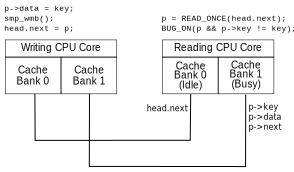
\includegraphics{memorder/Alpha}}
\caption{Why \tco{smp_read_barrier_depends()} is Required}
\label{fig:memorder:Why smp-read-barrier-depends() is Required}
\end{figure}

어떤 사람은 Alpha 가 포인터의 로드를 뒤따르는 의존적 로드에 대해 순서지키도록
강제하기 위해 포인터 로드와 디레퍼런스 사이에 \co{smp_rmb()} 를 위치시킬 수도
있을 겁니다.
하지만, 이는 읽기에 대해 data dependency 를 지키는 시스템들 (ARM, Itanium, PPC,
그리고 SPARC) 에는 불필요한 오버헤드를 가져올 수 있습니다.
그래서 이런 시스템에서의 오버헤드를 없애기 위해 \co{smp_read_barrier_depends()}
기능이 리눅스 커널에 추가되었습니다.
이 기능이
Listing~\ref{lst:memorder:Insert and Lock-Free Search} 의 line~19 에 추가될 수
있습니다만,
Listing~\ref{lst:memorder:Safe Insert and Lock-Free Search} 의 line~17 과~22 에
보여진 것처럼 \co{rcu_dereference()} 래퍼 매크로를 사용하는게 낫습니다.
\iffalse

One could place an \co{smp_rmb()} primitive
between the pointer fetch and dereference in order to force Alpha
to order the pointer fetch with the later dependent load.
However, this imposes unneeded overhead on systems (such as ARM,
Itanium, PPC, and SPARC) that respect data dependencies on the read side.
A \co{smp_read_barrier_depends()} primitive has therefore been added to the
Linux kernel to eliminate overhead on these systems.
This primitive could be inserted in place of line~19 of
Listing~\ref{lst:memorder:Insert and Lock-Free Search},
but it is better to use the \co{rcu_dereference()} wrapper macro
as shown on lines~17 and~22 of
Listing~\ref{lst:memorder:Safe Insert and Lock-Free Search}.
\fi

\co{smp_wmb()} 자리에 모든 읽기를 하는 CPU 들이 쓰기를 하는 CPU 의 쓰기를
순서대로 읽게 강제하는 소프트웨어 배리어를 구현할 수도 있을 겁니다.
하지만, 이 방법은 Alpha 와 같이 극단적으로 완화된 순서규칙을 갖는 CPU 에는
지나친 오버헤드를 갖게 하고, 더 나아가서 시스템이 강력한 real-time 응답 요구를
갖는 환경에서는 합리적인 방법으로 여겨지지 않기 때문에 리눅스 커뮤니티에서는
받아들여지지 않았습니다.
이 소프트웨어 배리어는 모든 다른 CPU에 inter-processor interrupt (IPI) 들을
보내는 것으로 구현될 수 있습니다.
그런 IPI 가 도착하면, CPU 는 메모리 배리어 인스트럭션을 수행해서 메모리 배리어
슛다운을 구현할 겁니다.
데드락을 막기 위해선 추가적인 로직이 필요합니다.
물론, data dependency 를 지켜주는 CPU 에서는 그런 배리어를 단순히
\co{smp_wmb()} 로 정의할 수 있을 겁니다.
Alpha 는 저무는 해인 만큼 미래에는 이런 방법이 다시 고려되어야겠습니다만,
2017년에 있어선 최신 리눅스 커널을 아끼는 DEC Alpha 시스템에서 돌리고 있는
사람들이 놀랍게도 많습니다.
\iffalse

It is also possible to implement a software barrier
that could be used in place of \co{smp_wmb()}, which would force
all reading CPUs to see the writing CPU's writes in order.
However, this approach was deemed by the Linux community
to impose excessive overhead
on extremely weakly ordered CPUs such as Alpha, and furthermore would
not be considered a reasonable approach by those whose systems must meet
aggressive real-time response requirements.
This software barrier could be implemented by sending inter-processor
interrupts (IPIs) to all other CPUs.
Upon receipt of such an IPI, a CPU would execute a memory-barrier
instruction, implementing a memory-barrier shootdown.
Additional logic is required to avoid deadlocks.
Of course, CPUs that respect data dependencies would define such a barrier
to simply be \co{smp_wmb()}.
Perhaps this decision should be revisited in the future as Alpha
fades off into the sunset, but as of 2017 there is a surprisingly
large number of people who run recent Linux kernels on their lovingly
preserved DEC Alpha systems.
\fi

\begin{listing}[tbp]
{ \scriptsize
\begin{verbbox}
 1  struct el *insert(long key, long data)
 2  {
 3      struct el *p;
 4      p = kmalloc(sizeof(*p), GFP_ATOMIC);
 5      spin_lock(&mutex);
 6      p->next = head.next;
 7      p->key = key;
 8      p->data = data;
 9      smp_wmb();
10      head.next = p;
11      spin_unlock(&mutex);
12  }
13
14  struct el *search(long key)
15  {
16      struct el *p;
17      p = rcu_dereference(head.next);
18      while (p != &head) {
19          if (p->key == key) {
20              return (p);
21          }
22          p = rcu_dereference(p->next);
23      };
24      return (NULL);
25  }
\end{verbbox}
}
\centering
\theverbbox
\caption{Safe Insert and Lock-Free Search}
\label{lst:memorder:Safe Insert and Lock-Free Search}
\end{listing}

리눅스 메모리 배리어 기능들은 그 이름을 Alpha 의 인스트럭션들에서 따왔는데,
\co{smp_mb()} 는 {\tt mb} 로부터, \co{smp_rmb()} 는 {\tt rmb} 로부터, 그리고
\co{smp_wmb()} 는 {\tt wmb} 로부터 왔습니다.
Alpha 는 \co{smp_read_barrier_depends()} 가 no-op 이 아니라 \co{smp_mb()} 인
유일한 CPU 입니다.
\iffalse

The Linux memory-barrier primitives took their names from the Alpha
instructions, so \co{smp_mb()} is {\tt mb}, \co{smp_rmb()} is {\tt rmb},
and \co{smp_wmb()} is {\tt wmb}.
Alpha is the only CPU where \co{smp_read_barrier_depends()} is
an \co{smp_mb()} rather than a no-op.
\fi

\QuickQuiz{}
	Alpha 의 \co{smp_read_barrier_depends()} 는 왜 \co{smp_rmb()} 가 아니라
	\co{smp_mb()} 죠?
	\iffalse

	Why is Alpha's \co{smp_read_barrier_depends()} an
	\co{smp_mb()} rather than \co{smp_rmb()}?
	\fi
\QuickQuizAnswer{
	먼저, Alpha 는 \co{mb} 와 \co{wmb} 인스트럭션만을 가지고 있어서,
	\co{smp_rmb()} 는 어떻든간에 Alpha 의 \co{mb} 인스트럭션으로 구현될
	겁니다.

	더 중요한건, \co{smp_read_barrier_depends()} 는 뒤따르는 스토어들을
	순서잡아야만 합니다.
	예를들어, 다음과 같은 코드를 고려해 봅시다:
	\iffalse

	First, Alpha has only \co{mb} and \co{wmb} instructions,
	so \co{smp_rmb()} would be implemented by the Alpha \co{mb}
	instruction in either case.

	More importantly, \co{smp_read_barrier_depends()} must
	order subsequent stores.
	For example, consider the following code:
	\fi

\vspace{5pt}
\begin{minipage}[t]{\columnwidth}
\small
\begin{verbatim}
  1 p = global_pointer;
  2 smp_read_barrier_depends();
  3 if (do_something_with(p->a, p->b) == 0)
  4   p->hey_look = 1;
\end{verbatim}
\end{minipage}
\vspace{5pt}

	여기서는 \co{p->a} 와 \co{p->b} 로부터의 로드만이 아니라
	\co{p->hey_look} 으로의 스토어도 순서가 잡혀져야만 합니다.
	\iffalse

	Here the store to \co{p->hey_look} must be ordered,
	not just the loads from \co{p->a} and \co{p->b}.
	\fi
} \QuickQuizEnd

Alpha 에 대한 더 자세한 정보를 위해선, 레퍼런스 매뉴얼~\cite{ALPHA2002} 을
참고하시기 바랍니다.
\iffalse

For more on Alpha, see its reference manual~\cite{ALPHA2002}.
\fi

\subsection{ARMv7-A/R}
\label{sec:memorder:ARMv7-A/R}

ARM 제품군의 CPU 는 임베디드 응용에서, 특히 휴대폰과 같이 전력 제한이 있는 응용
분야에서 굉장히 대중적으로 사용됩니다.
그 메모리 모델은 \Power{}(
(Section~\ref{sec:memorder:POWER / PowerPC} 을 참고하세요) 와 비슷합니다만, ARM
은 다른 메모리 배리어 인스트럭션 집합을 사용합니다~\cite{ARMv7A:2010}:
\iffalse

The ARM family of CPUs is extremely popular in embedded applications,
particularly for power-constrained applications such as cellphones.
Its memory model is similar to that of \Power{}
(see Section~\ref{sec:memorder:POWER / PowerPC}), but ARM uses a
different set of memory-barrier instructions~\cite{ARMv7A:2010}:
\fi

\begin{description}
\item	[\tco{DMB}] (data memory barrier) 는 특정 타입의 오퍼레이션들이 같은
	타입의 뒤따르는 모든 오퍼레이션들보다 먼저 완료된 것으로 \emph{보이게}
	합니다.
	오퍼레이션들의 ``타입'' 은 모든 오퍼레이션들이거나 쓰기만으로 제한될 수
	있습니다 (Alpha \co{wmb} 와 \Power{} \co{eieio} 인스트럭션과
	유사합니다).
	또한, ARM 은 캐시 일관성이 세가지 범위 중 하나를 가질 수 있게 합니다:
	싱글 프로세서, 프로세서들 중 일부 (``inner'') 그리고 글로벌
	(``outer'').
\iffalse

\item	[\tco{DMB}] (data memory barrier) causes the specified type of
	operations to \emph{appear} to have completed before any
	subsequent operations of the same type.
	The ``type'' of operations can be all operations or can be
	restricted to only writes (similar to the Alpha \co{wmb}
	and the \Power{} \co{eieio} instructions).
	In addition, ARM allows cache coherence to have one of three
	scopes: single processor, a subset of the processors
	(``inner'') and global (``outer'').
\fi
\item	[\tco{DSB}] (data synchronization barrier) 는 특정 타입의
	오퍼레이션들이 뒤따르는 (모든 타입의) 오퍼레이션들이 수행되기 전에
	정말로 완료되도록 만듭니다.
	오퍼레이션들의 ``타입'' 은 \co{DMB} 에서와 같습니다.
	\co{DSB} 인스트럭션은 ARM 아키텍쳐의 초기 버전에서는 \co{DWB} (drain
	write buffer 또는 data write barrier) 라고 불렸습니다.
\item	[\tco{ISB}] (instruction synchronization barrier) 는 CPU 파이프라인을
	비워서, \co{ISB} 를 뒤따르는 모든 인스트럭션들은 \co{ISB} 가 완료된
	후에야 불러들여집니다.
	예를 들어, 여러분이 (JIT 와 같은) 스스로를 수정하는 프로그램을
	만들었다면, 여러분은 해당 코드를 만들고 수행하기 전에 \co{ISB} 를
	수행해야만 합니다.
\iffalse

\item	[\tco{DSB}] (data synchronization barrier) causes the specified
	type of operations to actually complete before any subsequent
	operations (of any type) are executed.
	The ``type'' of operations is the same as that of \co{DMB}.
	The \co{DSB} instruction was called \co{DWB} (drain write buffer
	or data write barrier, your choice) in early versions of the
	ARM architecture.
\item	[\tco{ISB}] (instruction synchronization barrier) flushes the CPU
	pipeline, so that all instructions following the \co{ISB}
	are fetched only after the \co{ISB} completes.
	For example, if you are writing a self-modifying program
	(such as a JIT), you should execute an \co{ISB} between
	generating the code and executing it.
\fi
\end{description}

이 인스트럭션들 가운데 어떤 것도 리눅스의 \co{rmb()} 기능의 의미와 맞아떨어지지
않아서, 리눅스에서의 \co{rmb()} 는 완전한 \co{DMB} 로 구현되어집니다.
\co{DMB} 와 \co{DSB} 인스트럭션은 배리어의 앞과 뒤로 순서지어지는 액세스들의
재귀적 정의를 가지고 있는데, 이는 \Power{} 의 cumulativity 와 비슷한 효과를
갖습니다.

ARM 은 또한 control dependency 를 구현하고 있어서, 조건적 브랜치가 어떤 로드에
의존적이라면, 이 조건적 브랜치 뒤에 수행되는 모든 스토어는 이 로드 뒤로
순서지어집니다.
하지만, 조건적 브랜치를 뒤따르는 로드는 이 브랜치와 이 로드 사이에 \co{ISB}
인스트럭션이 있지 않다면 순서가 보장되지 \emph{않습니다}.
다음과 같은 예를 생각해 봅시다:
\iffalse

None of these instructions exactly match the semantics of Linux's
\co{rmb()} primitive, which must therefore be implemented as a full
\co{DMB}.
The \co{DMB} and \co{DSB} instructions have a recursive definition
of accesses ordered before and after the barrier, which has an effect
similar to that of \Power{}'s cumulativity.

ARM also implements control dependencies, so that if a conditional
branch depends on a load, then any store executed after that conditional
branch will be ordered after the load.
However, loads following the conditional branch will \emph{not}
be guaranteed to be ordered unless there is an \co{ISB}
instruction between the branch and the load.
Consider the following example:
\fi

\vspace{5pt}
\begin{minipage}[t]{\columnwidth}
\small
\begin{verbatim}
  1 r1 = x;
  2 if (r1 == 0)
  3   nop();
  4 y = 1;
  5 r2 = z;
  6 ISB();
  7 r3 = z;
\end{verbatim}
\end{minipage}
\vspace{5pt}

이 예에서, load-store control dependency 순서 규칙이 line~1 에서의 \co{x} 의
로드가 line~4 에서의 \co{y} 로의 스토어 앞으로 순서지어지게 합니다.
하지만, ARM 은 load-load control dependency 는 지켜주지 않으므로, line~1 에서의
로드는 line~5 에서의 로드 \emph{뒤에} 수행될 수도 있습니다.
다른 한편, line~2 에서의 조건적 브랜치는 line~6 에서의 \co{ISB} 인스트럭션과
결합되어 line~7 에서의 로드가 line~1 에서의 로드 뒤에 수행될 것을 보장합니다.
\co{ISB} 인스트럭션을 line~3 과~4 사이에 추가하면 line~1 과~5 사이의 순서가
강제될 것임을 알아두시기 바랍니다.
\iffalse

In this example, load-store control dependency ordering causes
the load from \co{x} on line~1 to be ordered before the store to
\co{y} on line~4.
However, ARM does not respect load-load control dependencies, so that
the load on line~1 might well happen \emph{after} the
load on line~5.
On the other hand, the combination of the conditional branch on line~2
and the \co{ISB} instruction on line~6 ensures that
the load on line~7 happens after the load on line~1.
Note that inserting an additional \co{ISB} instruction somewhere between
lines~3 and~4 would enforce ordering between lines~1 and~5.
\fi

\subsection{ARMv8}

\begin{figure}[tb]
\centering
\resizebox{2in}{!}{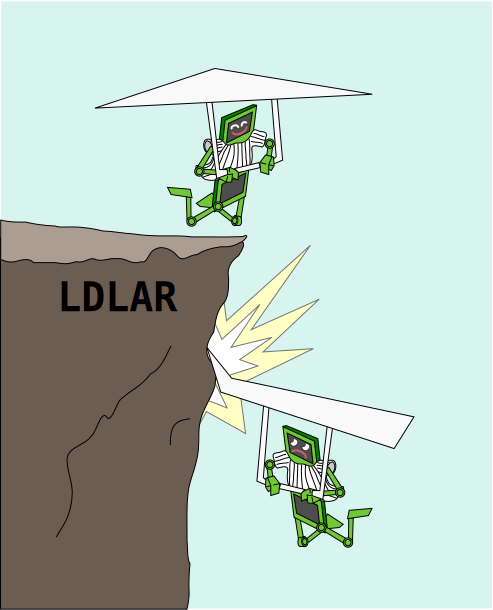
\includegraphics{cartoons/r-2014-LDLAR}}
\caption{Half Memory Barrier}
\ContributedBy{Figure}{fig:memorder:Half Memory Barrier}{Melissa Brossard}
\end{figure}

ARMv8 은 ARM 의 64-bit CPU~\cite{ARMv8A:2017} 로,
Section~\ref{sec:memorder:ARMv7-A/R} 에서 설명된 32-bit CPU 와 대조됩니다.
ARMv8 의 메모리 모델은 32-bit 에서의 것들과 비슷합니다만, load-acquire
(\co{LDLARB}, \co{LDLARH}, 그리고 \co{LDLAR}) 와 store-release (\co{STLLRB},
\co{STLLRH}, 그리고 \co{STLLR}) 인스트럭션들을 갖습니다.
이 인스트럭션들은 ``반쪽 메모리 배리어'' 로 동작해서,
Figure~\ref{fig:memorder:Half Memory Barrier} 로 그려진 것처럼 ARMv8 CPU 는
앞의 액세스들은 뒤의 \co{LDLAR} 인스트럭션과 재배치 할 수 있지만, 앞의
\co{LDLAR} 을 뒤의 액세스들과 재배치 하는건 금지되어 있습니다.
비슷하게, ARMv8 CPU 는 앞의 \co{STLLR} 인스트럭션을 뒤따르는 액세스들과
재배치하는건 가능하지만, 앞의 액세스들을 뒤따르는 \co{STLLR} 인스트럭션과
재배치하는건 금지되어 있습니다.
누군가는 예상했겠지만, 이는 이 인스트럭션들이 C11 의 load-acquire 와
store-release 를 바로 지원함을 의미합니다.
\iffalse

ARMv8 is ARM's 64-bit CPU~\cite{ARMv8A:2017},
in contrast to their 32-bit CPU described in
Section~\ref{sec:memorder:ARMv7-A/R}.
ARMv8's memory model closely resembles its 32-bit counterpart,
but adds load-acquire (\co{LDLARB}, \co{LDLARH}, and \co{LDLAR})
and store-release (\co{STLLRB}, \co{STLLRH}, and \co{STLLR})
instructions.
These instructions act as ``half memory barriers'', so that
ARMv8 CPUs can reorder previous accesses with a later \co{LDLAR}
instruction, but are prohibited from reordering an earlier \co{LDLAR}
instruction with later accesses, as fancifully depicted in
Figure~\ref{fig:memorder:Half Memory Barrier}.
Similarly, ARMv8 CPUs can reorder an earlier \co{STLLR} instruction with
a subsequent access, but are prohibited from reordering
previous accesses with a later \co{STLLR} instruction.
As one might expect, this means that these instructions directly support
the C11 notion of load-acquire and store-release.
\fi

하지만, ARMv8 은 많은 환경에서 store-release 와 load-acquire 가 완전한 배리어로
동작하도록 조합할 것을 필수로 함으로써 C11 메모리 모델 이상의 것을 할수도
있습니다.
예를 들어, ARMv8 에서, 스토어 뒤에 store-release, load-acquire, 로드가 모두
서로 다른 변수들에 대해 행해지며 순서대로 뒤따른다면, 모든 CPU 들은 최초의
스토어가 마지막의 로드를 앞선다는데에 동의하게 됩니다.
흥미롭게도, 대부분의 (x86 과 mainframe 을 포함해서) TSO 아키텍쳐들은 이 보장을
갖지 않아서, 두개의 로드가 두개의 스토어 앞으로 재배치 될 수 있게 합니다.

ARMv8 은 또한 제조사가 공개적으로 정형적 모델을 통해 그 메모리 순서 규칙을
정의한 첫번째 CPU 의 영예를 가졌습니다.
\iffalse

However, ARMv8 goes well beyond the C11 memory model by mandating that
the combination of a store-release and load-acquire act as a full
barrier under many circumstances.
For example, in ARMv8, given a store followed by a store-release followed
a load-acquire followed by a load, all to different variable, all CPUs
would agree that the initial store preceded the final load.
Interestingly enough, most TSO architectures (including x86 and the
mainframe) do not make this guarantee, as the two loads could be
reordered before the two stores.

ARMv8 also has the distinction of being the first CPU whose vendor publicly
defined its memory ordering with a formal model~\cite{ARMv8A:2017}.
\fi

\subsection{Itanium}

Itanium 은 완화된 일관성 모델을 제공해서, 명시적인 메모리 배리어 인스트럭션이
없으면, Itanium 은 임의적으로 메모리 레퍼런스들을 재배치 할 수
있습니다~\cite{IntelItanium02v2}.
Itanium 은 {\tt mf} 라는 이름의 memory-fence 인스트럭션을 갖습니다만, 또한
로드, 스토어, 그리고 일부 어토믹 인스트럭션들을 ``반쪽짜리 memory fence'' 로
변환하는 변경자 또한 갖습니다~\cite{IntelItanium02v2}.
{\tt acq} 변경자는 뒤따르는 메모리 레퍼런스 인스트럭션들이 {\tt acq} 앞으로
재배치 되는 것을 막습니다만, 앞의 메모리 레퍼런스 인스트럭션들이 {\tt acq} 뒤로
재배치 되는건 허용하는데, 이는 ARMv8 의 load-acquire 인스트럭션과 유사합니다.
비슷하게, {\tt rel} 변경자는 앞의 메모리 레퍼런스 인스트럭션들이 {\tt rel} 뒤로
재배치 되는걸 막습니다만, 뒤따르는 메모리 레퍼런스 인스트럭션들이 {\tt rel}
앞으로 재배치되는건 허용합니다.
\iffalse

Itanium offers a weak consistency model, so that in absence of explicit
memory-barrier instructions, Itanium is within its rights to arbitrarily
reorder memory references~\cite{IntelItanium02v2}.
Itanium has a memory-fence instruction named {\tt mf}, but also has
``half-memory fence'' modifiers to loads, stores, and to some of its atomic
instructions~\cite{IntelItanium02v3}.
The {\tt acq} modifier prevents subsequent memory-reference instructions
from being reordered before the {\tt acq}, but permits
prior memory-reference instructions to be reordered after the {\tt acq},
similar to the ARMv8 load-acquire instructions.
Similarly, the {\tt rel} modifier prevents prior memory-reference
instructions from being reordered after the {\tt rel}, but allows
subsequent memory-reference instructions to be reordered before
the {\tt rel}.
\fi

이런 반쪽짜리 memory fence 들은 크리티컬 섹션에 유용한데, 오퍼레이션들을
크리티컬 섹션 안으로 들여보내는건 안전하지만 크리티컬 섹션 밖으로 내보내는건
치명적일 수 있기 때문입니다.
하지만, 이 기능을 가진 CPU 가운데 하나로써,\footnote{
	ARMv8 은 최근에 load-acquire 와 store-release 인스트럭션을
	추가했습니다.}
Itanium 은 리눅스의 락 획득과 해제에 관련된 메모리 순서 규칙을 정의합니다.
이상하게 들릴 수 있지만, 실제 Itanium 하드웨어는 load-acquire 와 store-release
인스트럭션들을 완전한 배리어로 구현했다는 소문이 있습니다.
어쨌든, Itanium 은 load-acquire 와 store-release 의 (소문이 사실이어서 실제가
아니라면) 개념을 인스트럭션 집합에 추가한 첫번째 주류 CPU 였습니다.
\iffalse

These half-memory fences are useful for critical sections, since
it is safe to push operations into a critical section, but can be
fatal to allow them to bleed out.
However, as one of the few CPUs with this property, Itanium at one
time defined Linux's semantics of memory ordering associated with lock
acquisition and release.\footnote{
	PowerPC is now the architecture having this dubious privilege.}
Oddly enough, actual Itanium hardware is rumored to implement
both load-acquire and store-release instructions as full barriers.
Nevertheless, Itanium was the first mainstream CPU to introduce the concept
(if not the reality) of load-acquire and store-release into its
instruction set.
\fi

Itanium {\tt mf} 인스트럭션은 리눅스 커널의 \co{smp_rmb()}, \co{smp_mb()},
그리고 \co{smp_wmb()} 기능에 사용됩니다.
아, 그리고 반대의 루머가 있긴 하지만, ``mf'' 는 ``memory fence'' 의 약자가
맞습니다.

마지막으로, Itanium 은 ``mf'' 인스트럭션을 포함해 ``release'' 오퍼레이션들에
글로벌하고 완전한 순서를 제공합니다.
이는 transitivity 를 제공하는데, 이는 특정 코드 조각이 특정 액세스가 일어난
것으로 파악했다면, 뒤따르는 모든 코드 조각은 역시 이 액세스가 이미 일어난
것으로 보게 됨을 의미합니다.
다시 말하지만, 모든 관련된 코드 조각들이 올바르게 메모리 배리어를 사용했다는
가정 하의 이야기 입니다.
\iffalse

The Itanium {\tt mf} instruction is used for the \co{smp_rmb()},
\co{smp_mb()}, and \co{smp_wmb()} primitives in the Linux kernel.
Oh, and despite rumors to the contrary, the ``mf'' mnemonic really
does stand for ``memory fence''.

Finally, Itanium offers a global total order for ``release'' operations,
including the ``mf'' instruction.
This provides the notion of transitivity, where if a given code fragment
sees a given access as having happened, any later code fragment will
also see that earlier access as having happened.
Assuming, that is, that all the code fragments involved correctly use
memory barriers.
\fi

\subsection{MIPS}

MIPS 메모리 모델~\cite[Table 6.6]{MIPSvII-A-2015} 은 ARM, Itanium, 그리고
\Power{} 를 닮아서, 기본적으로는 완화된 순서를 갖지만, 의존성은 지켜줍니다.
MIPS 는 다양한 메모리 배리어 인스트럭션을 갖습니다만, 하드웨어 상의 필요에
매여있기보다는 ARM64 에 추가된 것들과 비슷하게, 리눅스 커널과 C++11
표준~\cite{RichardSmith2015N4527} 에서 존재하는 사용상의 경우에 연결되어
있습니다:
\iffalse

The MIPS memory model~\cite[page~479]{MIPSvII-A-2017}
appears to resemble that of ARM, Itanium, and \Power{},
being weakly ordered by default, but respecting dependencies.
MIPS has a wide variety of memory-barrier instructions, but ties them
not to hardware considerations, but rather to the use cases provided
by the Linux kernel and the C++11 standard~\cite{RichardSmith2015N4527}
in a manner similar to the ARM64 additions:
\fi

\begin{description}[style=nextline]
\item[\tco{SYNC}]
	메모리 레퍼런스 외에도 여러 하드웨어 오퍼레이션들을 위한 완전한 배리어.
	\iffalse

	Full barrier for a number of hardware operations in addition
	% TODO
	to memory references, which is used to implement the v4.13
	Linux kernel's \co{smp_mb()} for OCTEON systems.
	to memory references.
	\fi
\item[\tco{SYNC_WMB}]
	리눅스 커널의 \co{smp_wmb()} 기능을 구현하는데 사용될 수 있는 쓰기
	메모리 배리어.
	\iffalse

	% TODO
	Write memory barrier, which can be used on OCTEON systems
	to implement the
	\co{smp_wmb()} primitive in the v4.13 Linux kernel via the
	\co{syncw} mnemonic.
	Other systems use plain \co{sync}.
	\fi
\item[\tco{SYNC_MB}]
	메모리 오퍼레이션들에만 작동하는 완전한 메모리 배리어.
	이는 리눅스 커널의 \co{smp_mb()} 와 C++
	\co{atomic_thread_fence(memory_order_seq_cst)} 의 구현에 사용될 수
	있습니다.
	\iffalse

	Full memory barrier, but only for memory operations.
	This may be used to implement the 
	C++ \co{atomic_thread_fence(memory_order_seq_cst)}.
	\fi
\item[\tco{SYNC_ACQUIRE}]
	리눅스 커널의 \co{smp_load_acquire()} 와 C++
	\co{atomic_load_explicit(..., memory_order_acquire)} 의 구현에 사용될
	수 있는 acquire 메모리 배리어.
	\iffalse

	Acquire memory barrier, which could be used to implement
	C++'s \co{atomic_thread_fence(memory_order_acquire)}.
	In theory, it could also be used to implement the v4.13 Linux-kernel
	\co{smp_load_acquire()} primitive, but in practice
	\co{sync} is used instead.
	\fi
\item[\tco{SYNC_RELEASE}]
	리눅스 커널의 \co{smp_store_release()} 와 C++
	\co{atomic_store_explicit(..., memory_order_release)} 의 구현에 사용될
	수 있는 release 메모리 배리어.
	\iffalse

	Release memory barrier, which may be used to implement
	C++'s \co{atomic_thread_fence(memory_order_release)}.
	In theory, it could also be used to implement the v4.13 Linux-kernel
	\co{smp_store_release()} primitive, but in practice
	\co{sync} is used instead.
	\fi
\item[\tco{SYNC_RMB}]
	리눅스 커널의 \co{smp_rmb()} 기능을 구현하는데 사용될 수 있는 읽기
	메모리 배리어.
	\iffalse

	Read memory barrier, which could in theory be used to implement the
	\co{smp_rmb()} primitive in the Linux kernel, except that current
	MIPS implementations supported by the v4.13 Linux kernel do not
	need an explicit instruction to force ordering.
	Therefore, \co{smp_rmb()} instead simply constrains the compiler.
	\fi
% TODO
\item[\tco{SYNCI}]
	Instruction-cache synchronization, which is used in conjunction with
	other instructions to allow self-modifying code, such as that produced
	by just-in-time (JIT) compilers.
\end{description}

MIPS 설계자들과의 비공식적 토론은 MIPS 가 ARM 과 \Power{} 의 것과 유사한
transitivity 또는 cumulativity 에 대한 정의를 가짐을 암시합니다.
하지만, 서로 다른 MIPS 구현들은 서로 다른 메모리 순서 규칙을 가질 수 있으며,
따라서 여러분이 사용하고 있는 특정 MIPS 구현의 문서를 확인하는게 중요합니다.
\iffalse

Informal discussions with MIPS architects indicates that MIPS has a
definition of transitivity or cumulativity similar to that of
ARM and \Power{}.
However, it appears that different MIPS implementations can have
different memory-ordering properties, so it is important to consult
the documentation for the specific MIPS implementation you are using.
\fi

\subsection{PA-RISC}

PA-RISC 아키텍쳐는 로드와 스토어의 완전한 재배치를 허용하지만, 실제 CPU 들은
완전히 순서를 지켜줍니다~\cite{GerryKane96a}.
이는 리눅스 커널의 메모리 순서 보장 기능들이 아무 코드도 생성하지 않음을
의미하지만, 코드를 메모리 배리어 앞뒤로 재배치 하는 컴파일러 최적화를
불가능하게 하기 위해 \GCC 의 {\tt memory} 기능은 사용합니다.
\iffalse

Although the PA-RISC architecture permits full reordering of loads and
stores, actual CPUs run fully ordered~\cite{GerryKane96a}.
This means that the Linux kernel's memory-ordering primitives generate
no code, however, they do use \GCC's {\tt memory} attribute to disable
compiler optimizations that would reorder code across the memory
barrier.
\fi

\subsection{\Power{} / PowerPC}
\label{sec:memorder:POWER / PowerPC}

\Power{} 와 PowerPC\textsuperscript{\textregistered} CPU 제품군은 다양한 메모리
배리어 인스트럭션을 갖습니다~\cite{PowerPC94,MichaelLyons05a}:
\iffalse

The \Power{} and PowerPC\textsuperscript{\textregistered}
CPU families have a wide variety of memory-barrier
instructions~\cite{PowerPC94,MichaelLyons05a}:
\fi
\begin{description}
\item	[\tco{sync}] 는 모든 앞서는 오퍼레이션들이 뒤따르는 오퍼레이션들이
	시작하기 전에 완료된 것으로 {\em 보이게} 합니다.
	따라서 이 인스트럭션은 상당히 비용이 비쌉니다.
\item	[\tco{lwsync}] (light-weight sync) 는 로드를 뒤의 로드와 스토어에 대해,
	그리고 스토어를 뒤의 스토어에 대해 순서 맞춥니다.
	하지만, 이 인스트럭션은 스토어를 뒤따르는 로드에 대해 순서맞추지는 {\em
	않습니다}.
	흥미롭게도, {\tt lwsync} 인스트럭션은 zSeries 와, 그리고 우연히도,
	SPARC TSO 와 같은 순서 규칙을 강제합니다.
	\co{lwsync} 인스트럭션은 load-acquire 와 store-release 오퍼레이션들을
	구현하는데 사용될 수 있습니다.
\iffalse
\item	[\tco{sync}] causes all preceding operations to {\em appear to have}
	completed before any subsequent operations are started.
	This instruction is therefore quite expensive.
\item	[\tco{lwsync}] (light-weight sync) orders loads with respect to
	subsequent loads and stores, and also orders stores.
	However, it does {\em not} order stores with respect to subsequent
	loads.
	The \co{lwsync} instruction may be used to implement
	load-acquire and store-release operations.
	% TODO
	Interestingly enough, the {\tt lwsync} instruction enforces
	the same within-CPU ordering as does x86, z~Systems, and coincidentally,
	SPARC TSO.
	However, placing the \co{lwsync} instruction between each
	pair of memory-reference instructions will \emph{not}
	result in x86, z~Systems, or SPARC TSO memory ordering.
	On these other systems, if a pair of CPUs independently execute
	stores to different variables, all other CPUs will agree on the
	order of these stores.
	Not so on PowerPC, even with an \co{lwsync} instruction between each
	pair of memory-reference instructions, because PowerPC is
	non-multicopy atomic.
\fi
\item	[\tco{eieio}] (enforce in-order execution of I/O) 는 모든 앞의 캐시
	가능한 스토어들을 뒤따르는 스토어보다 먼저 완료된 것으로 보이게 합니다.
	하지만, 캐시 가능한 메모리로의 스토어들은 캐시 가능하지 않은 메모리로의
	스토어들과 따로 순서지어져서, {\tt eieio} 는 MMIO 스토어가 스핀락
	해제보다 앞서게 강제하지는 않을 겁니다.
\item	[\tco{isync}] 는 모든 앞의 인스트럭션들이 뒤따르는 인스트럭션들이
	수행을 시작하기 전에 완료된 것으로 보이게 합니다.
	이는 앞의 인스트럭션들은 그들이 만들어낼 수 있는 모든 trap 들은 이미
	일어났거나 일어나지 않을 것이 보장될 정도로, 그리고 이 인스트럭션들의
	부가적 효과들 (예를 들면, page-table 의 변경) 은 뒤따르는
	인스트럭션들에게 보일 정도로 많이 진행되었어야 함을 의미합니다.
\iffalse

\item	[\tco{eieio}] (enforce in-order execution of I/O, in case you
	were wondering) causes all preceding cacheable stores to appear
	to have completed before all subsequent stores.
	However, stores to cacheable memory are ordered separately from
	stores to non-cacheable memory, which means that {\tt eieio}
	will not force an MMIO store to precede a spinlock release.
\item	[\tco{isync}] forces all preceding instructions to appear to have
	completed before any subsequent instructions start execution.
	This means that the preceding instructions must have progressed
	far enough that any traps they might generate have either happened
	or are guaranteed not to happen, and that any side-effects of
	these instructions (for example, page-table changes) are seen by the
	subsequent instructions.
\fi
\end{description}

불행히도 이 인스트럭션들 중 어느 것도 {\em 모든} 스토어들이 순서지어져야
하지만, {\tt sync} 인스트럭션의 높은 오버헤드를 갖는 동작을 필요로 하지는 않는
리눅스의 {\tt wmb()} 기능에 정확히 맞아떨어지지 않습니다.
하지만 선택의 여지가 없습니다: ppc64 버전의 {\tt wmb()} 와 {\tt mb()} 는 무거운
{\tt sync} 인스트럭션으로 정의되어 있습니다.
하지만, 리눅스의 \co{smp_wmb()} 인스트럭션은 (드라이버는 SMP 커널에서는
물론이고 UP 에서도 MMIO 들의 순서를 세심히 지켜줘야 하기 때문에) MMIO 에 절대
사용되지 않으므로, 더 가벼운 {\tt eieio} 인스트럭션으로 정의되어 있습니다.
이 인스트럭션은 다섯개의 모음으로 구성된 약자를 가진다는 점에서도 독특합니다.
\co{smp_mb()} 인스트럭션 또한 {\tt sync} 인스트럭션으로 정의되어 있습니다만,
\co{smp_rmb()} 와 \co{rmb()} 모두 더 가벼운 {\tt lwsync} 인스트럭션으로
정의되어 있습니다.
\iffalse

Unfortunately, none of these instructions line up exactly with Linux's
{\tt wmb()} primitive, which requires {\em all} stores to be ordered,
but does not require the other high-overhead actions of the {\tt sync}
instruction.
But there is no choice: ppc64 versions of {\tt wmb()} and {\tt mb()} are
defined to be the heavyweight {\tt sync} instruction.
However, Linux's \co{smp_wmb()} instruction is never used for MMIO
(since a driver must carefully order MMIOs in UP as well as
SMP kernels, after all), so it is defined to be the lighter weight
{\tt eieio} instruction.
This instruction may well be unique in having a five-vowel mnemonic.
The \co{smp_mb()} instruction is also defined to be the {\tt sync}
instruction, but both \co{smp_rmb()} and \co{rmb()} are defined to
be the lighter-weight {\tt lwsync} instruction.
\fi

\Power{} 는 transitivity 를 얻는데 사용될 수 있는 ``cumulativity'' 를 갖추고
있습니다.
제대로 사용되면, 앞의 코드 조각의 결과를 보는 모든 코드는 이 앞의 코드 조각들이
스스로 본 액세스들 역시 볼 것입니다.
더 많은 자세한 내용은 McKenney 와 Silvera 의 글~\cite{PaulEMcKenneyN2745r2009}
에서 볼 수 있습니다.

\Power{} 는 ARM 과 같은 방식으로 control dependency 를 지키는데, ARM \co{ISB}
인스트럭션이 \Power{} \co{isync} 인스트럭션으로 바뀌어야 한다는 점은
예외입니다.
\iffalse

\Power{} features ``cumulativity'', which can be used to obtain
transitivity.
When used properly, any code seeing the results of an earlier
code fragment will also see the accesses that this earlier code
fragment itself saw.
Much more detail is available from
McKenney and Silvera~\cite{PaulEMcKenneyN2745r2009}.

\Power{} respects control dependencies in much the same way that ARM
does, with the exception that the \Power{} \co{isync} instruction
is substituted for the ARM \co{ISB} instruction.
\fi

\Power{} 아키텍쳐의 많은 멤버들이 일관적이지 않은 인스트럭션 캐시를 가져서,
메모리로의 스토어는 인스트럭션 캐시에는 반영되지 않을 수도 있습니다.
고맙게도, 오늘날엔 적은 사람들만이 스스로를 수정하는 코드를 작성합니다만, JIT
과 컴파일러는 항상 이 일을 합니다.
더 나아가서, 최근에 수행된 프로그램을 다시 컴파일 하는 행위는 CPU 의 관점에서는
스스로를 수정하는 코드처럼 보입니다.
{\tt icbi} 인스트럭션 (instruction cache block invalidate) 는 인스트럭션
캐시로부터 특정 캐시 라인을 무효화 시키고, 이런 상황에서 사용될 수 있습니다.
\iffalse

Many members of the \Power{} architecture have incoherent instruction
caches, so that a store to memory will not necessarily be reflected
in the instruction cache.
Thankfully, few people write self-modifying code these days, but JITs
and compilers do it all the time.
Furthermore, recompiling a recently run program looks just like
self-modifying code from the CPU's viewpoint.
The {\tt icbi} instruction (instruction cache block invalidate)
invalidates a specified cache line from
the instruction cache, and may be used in these situations.
\fi

\subsection{SPARC RMO, PSO, and TSO}

SPARC 에서의 Solaris 는 리눅스가 ``sparc'' 32-bit 아키텍쳐로 빌드되었을 때와
같이 TSO (total-store order) 를 사용합니다.
하지만, 64-bit 리눅스 커널 (``sparc64'' 아키텍쳐) 는 SPARC 를 RMO
(relaxed-memory order) 모델~\cite{SPARC94} 로 돌아갑니다.
SPARC 아키텍쳐는 또한 중간적 PSO (partial store order) 를 제공합니다.
RMO 에서 돌아가는 모든 프로그램은 PSO 나 TSO 에서도 돌아갈 수 있으며, 비슷하게,
PSO 에서 돌아가는 프로그램은 TSO 에서도 돌아갑니다.
공유 메모리 병렬 프로그램을 다른 방향으로 옮겨 수행하는 것은 메모리 배리어의
주의 깊은 추가를 필요로 합니다만, 앞에서도 이야기 되었듯, 동기화 도구의 표준적
사용을 하는 프로그램은 메모리 배리어에 대해 걱정할 필요가 없을 겁니다.

SPARC 는 세세한 수준의 규칙 보장 제어를 가능하게 하는, 매우 유연한 메모리
배리어 인스트럭션~\cite{SPARC94} 을 갖습니다.
\iffalse

Solaris on SPARC uses TSO (total-store order), as does Linux when built for
the ``sparc'' 32-bit architecture.
However, a 64-bit Linux kernel (the ``sparc64'' architecture)
runs SPARC in RMO (relaxed-memory order) mode~\cite{SPARC94}.
The SPARC architecture also offers an intermediate PSO (partial store
order).
Any program that runs in RMO will also run in either PSO or TSO, and similarly,
a program that runs in PSO will also run in TSO.
Moving a shared-memory parallel program in the other direction may
require careful insertion of memory barriers, although, as noted earlier,
programs that make standard use of synchronization primitives need not
worry about memory barriers.

SPARC has a very flexible memory-barrier instruction~\cite{SPARC94}
that permits fine-grained control of ordering:
\fi
\begin{description}
\item	[\tco{StoreStore}] 는 앞의 스토어들을 뒤따르는 스토어들에 대해
	순서지어줍니다.
	(이 옵션은 리눅스 \co{smp_wmb()} 기능에서 사용됩니다.)
\item	[\tco{LoadStore}] 는 앞의 로드를 뒤따르는 스토어에 대해 순서지어줍니다.
\item	[\tco{StoreLoad}] 는 앞의 스토어들을 뒤따르는 로드들에 대해
	순서지어줍니다.
\item	[\tco{LoadLoad}] 는 앞의 로드를 뒤따르는 로드들에 대해 순서지어줍니다.
	(이 옵션은은 리눅스 \co{smp_rmb()} 기능에 의해 사용됩니다.)
\item	[\tco{sync}] 는 모든 앞의 오퍼레이션들을 뒤따르는 오퍼레이션들 전에
	완료되도록 합니다.
\item	[\tco{MemIssue}] 는 진행중인 메모리 오퍼레이션들이 뒤따르는 메모리
	오퍼레이션들 전에 완료되게 하는데, memory-mapped I/O 의 일부 경우에
	중요합니다.
\item	[\tco{Lookaside}] 는 MemIssue 와 동일하지만, 앞의 스토어들과 뒤따르는
	로드들에만 적용되며, 같은 메모리 영역에 접근하는 스토어와 로드에만
	적용됩니다.
\iffalse

\item	[\tco{StoreStore}] orders preceding stores before subsequent stores.
	(This option is used by the Linux \co{smp_wmb()} primitive.)
\item	[\tco{LoadStore}] orders preceding loads before subsequent stores.
\item	[\tco{StoreLoad}] orders preceding stores before subsequent loads.
\item	[\tco{LoadLoad}] orders preceding loads before subsequent loads.
	(This option is used by the Linux \co{smp_rmb()} primitive.)
\item	[\tco{Sync}] fully completes all preceding operations before starting
	any subsequent operations.
\item	[\tco{MemIssue}] completes preceding memory operations before subsequent
	memory operations, important for some instances of memory-mapped
	I/O.
\item	[\tco{Lookaside}] does the same as MemIssue,
	but only applies to preceding stores
	and subsequent loads, and even then only for stores and loads that
	access the same memory location.
\fi
\end{description}

리눅스 \co{smp_mb()} 기능은 앞의 네개의 옵션들을 함께 사용하는데, 따라서
\co{membar #LoadLoad | #LoadStore | #StoreStore | #StoreLoad} 는 완전한 메모리
오퍼레이션들의 순서 보장을 제공합니다.
\iffalse

The Linux \co{smp_mb()} primitive uses the first four options together,
as in
\co{membar #LoadLoad | #LoadStore | #StoreStore | #StoreLoad},
thus fully ordering memory operations.
\fi

그런데, \qco{membar #MemIssue} 는 왜 필요할까요?
\qco{membar #StoreLoad} 는 뒤따르는 로드가 그 값을 스토어 버퍼에서 가져올 수
있게 해서, 해당 쓰기가 MMIO 레지스터로 향하는 것이어서 읽히는 값에 따라
부가작용을 일으킬 수 있는 것이라면 문제가 될 수 있습니다.
반면에, \qco{membar #MemIssue} 는 이 로드가 수행되기 전에 스토어 버퍼들이
비워지게 해서, 이 로드는 이 값을 실제로 MMIO 레지스터로부터 얻어오게 할 겁니다.
드라이버는 이대신 \qco{membar #Sync} 를 사용할 수 있습니다만, 더 비싼
\qco{membar #Sync} 의 추가적인 동작이 필요없는 경우엔 더 가벼운 편인
\qco{membar #MemIssue} 가 낫습니다.
\iffalse

So, why is \qco{membar #MemIssue} needed?
Because a \qco{membar #StoreLoad} could permit a subsequent
load to get its value from a store buffer, which would be
disastrous if the write was to an MMIO register that induced side effects
on the value to be read.
In contrast, \qco{membar #MemIssue} would wait until the store buffers
were flushed before permitting the loads to execute,
thereby ensuring that the load actually gets its value from the MMIO register.
Drivers could instead use \qco{membar #Sync}, but the lighter-weight
\qco{membar #MemIssue} is preferred in cases where the additional function
of the more-expensive \qco{membar #Sync} are not required.
\fi

\qco{membar #Lookaside} 는 \qco{membar #MemIssue} 의 경량 버전으로, 특정 MMIO
레지스터에 쓰기를 하는 행위가 해당 레지스터로부터 다음에 읽힐 값에 영향을 주는
경우에 유용합니다.
하지만, 더 무거운 \qco{membar #MemIssue} 는 해당 MMIO 레지스터로의 쓰기가
나중에 {\em 다른} MMIO 레지스터로부터의 읽기에 영향을 끼치는 경우에는 반드시
사용되어야만 합니다.

SPARC 가 왜 \co{wmb()} 가 \qco{membar #MemIssue} 가 되게, 그리고 \co{smp_wmb()}
가 \qco{membar #StoreStore} 로 되도록 정의하지 않아서 현재의 정의는 일부
드라이버에서는 버그에 취약하도록 만들었는지는 분명치 않습니다.
리눅스가 수행되는 모든 SPARC CPU 들은 아키텍쳐에서 허용하는 것보다 더 보수적인
메모리 순서 보장 모델을 구현했을 가능성이 큽니다.
\iffalse

The \qco{membar #Lookaside} is a lighter-weight version of
\qco{membar #MemIssue}, which is useful when writing to a given MMIO register
affects the value that will next be read from that register.
However, the heavier-weight \qco{membar #MemIssue} must be used when
a write to a given MMIO register affects the value that will next be
read from {\em some other} MMIO register.

It is not clear why SPARC does not define \co{wmb()} to be
\qco{membar #MemIssue} and \co{smp_wmb()} to be
\qco{membar #StoreStore},
as the current definitions seem vulnerable to bugs in some drivers.
It is quite possible that all the SPARC CPUs that Linux runs on
implement a more conservative memory-ordering model than the architecture
would permit.
\fi

SPARC 는 {\tt flush} 인스트럭션이 인스트럭션이 스토어된 시점과 수행되는 시점
사이에서 사용될 것을 필요로 합니다~\cite{SPARC94}.
이는 SPARC 의 인스트럭션 캐시로부터 해당 지역의 기존 값을 비우기 위해
필요합니다.
{\tt flush} 는 주소를 받아서, 인스트럭션 캐시로부터 해당 위치의 값만을 지운다는
것을 알아두시기 바랍니다.
SMP 시스템에서는 모든 CPU 의 캐시가 비워지지만, 언제 모든 CPU 의 플러시가
완료되었는지를 알아낼 간편한 방법은 없습니다만, 구현상의 레퍼런스는 있습니다.
\iffalse

SPARC requires a {\tt flush} instruction be used between the time that
an instruction is stored and executed~\cite{SPARC94}.
This is needed to flush any prior value for that location from
the SPARC's instruction cache.
Note that {\tt flush} takes an address, and will flush only that address
from the instruction cache.
On SMP systems, all CPUs' caches are flushed, but there is no
convenient way to determine when the off-CPU flushes complete,
though there is a reference to an implementation note.
\fi

\subsection{x86}

x86 CPU 는 ``process ordering'' 을 제공해서, 모든 CPU 가 특정 CPU 의 메모리로의
쓰기의 순서에 동의하게 하므로, \co{smp_wmb()} 기능은 이 CPU 에서는 no-op 이
됩니다~\cite{IntelXeonV3-96a}.
하지만, 컴파일러가 \co{smp_wmb()} 기능의 앞뒤를 재배치 하는 최적화를 수행하는
걸 막기 위한 컴파일러 지시어는 필요합니다.

한편, x86 CPU 들은 전통적으로 로드에 대해서는 순서 보장을 제공하지 않았으므로,
\co{smp_mb()} 와 \co{smp_rmb()} 기능은 {\tt lock;addl} 로 확장됩니다.
이 어토믹 인스트럭션은 로드와 스토어 모두에 대한 배리어로 동작합니다.
\iffalse

Since the x86 CPUs provide ``process ordering'' so that all CPUs agree
on the order of a given CPU's writes to memory, the \co{smp_wmb()} primitive
is a no-op for the CPU~\cite{IntelXeonV3-96a}.
However, a compiler directive is required to
prevent the compiler from performing optimizations that would result
in reordering across the \co{smp_wmb()} primitive.

On the other hand, x86 CPUs have traditionally given
no ordering guarantees for loads, so
the \co{smp_mb()} and \co{smp_rmb()} primitives expand to {\tt lock;addl}.
This atomic instruction acts as a barrier to both loads and stores.
\fi

Intel 은 또한 x86 을 위한 메모리 모델을
공개했습니다~\cite{Intelx86MemoryOrdering2007}.
이로 인해 Intel 의 실제 CPU 들은 기존의 명세서들에서 이야기하던 것보다 더
빡빡한 순서 규칙을 강제한다는 것이 드러났으며, 따라서 이 모델은 단순히 기존의
실질적 표준의 행동을 의무화 합니다.
더 최근에, Intel 은 x86 을 위한 개정된 메모리 모델~\cite[Section
8.2]{Intel64IA32v3A2011} 를 공개했는데, 여기선 스토어에 대해선 완전한 전역적
순서를 의무화합니다만, 개별 CPU 는 여전히 스스로의 스토어들을 이 완전한 전역적
순서보다 빠르게 발생한 것으로 볼 수 있게 합니다.
완전한 순서 보장에 대한 이 예외는 스토어 버퍼들에 관련된 중요한 하드웨어
최적화를 허용하기 위해 필요합니다.
또한, 메모리 순서 보장 규칙은 인과성을 준수해서, CPU~0 가 CPU~1 에 의한
스토어를 봤다면, CPU~0 는 CPU~1 이 해당 스토어 전에 본 모든 스토어들 역시 볼 수
있을 것을 보장합니다.
소프트웨어는 이 하드웨어 최적화들을 무시하기 위해 어토믹 오퍼레이션들을 사용할
수도 있는데, 이는 어토믹 오퍼레이션들이 어토믹하지 않은 비슷한 것들에 비해 더
비싼 경향을 갖는 이유입니다.
이 전체 스토어 순서는 기존 프로세서들에서는 보장되지 \emph{않습니다}.
\iffalse

Intel has also published a memory model for
x86~\cite{Intelx86MemoryOrdering2007}.
It turns out that Intel's actual CPUs enforced tighter ordering than
was claimed in the previous specifications, so this model is in effect
simply mandating the earlier de-facto behavior.
Even more recently, Intel published an updated memory model for
x86~\cite[Section 8.2]{Intel64IA32v3A2011}, which mandates a total global order
for stores, although individual CPUs are still permitted to see their
own stores as having happened earlier than this total global order
would indicate.
This exception to the total ordering is needed to allow important
hardware optimizations involving store buffers.
In addition, memory ordering obeys causality, so that if CPU~0 sees a
store by CPU~1, then CPU~0 is guaranteed to see all stores that CPU~1
saw prior to its store.
Software may use atomic operations to override these hardware optimizations,
which is one reason that atomic operations tend to be more expensive
than their non-atomic counterparts.
This total store order is \emph{not} guaranteed on older processors.
\fi

특정 메모리 위치에 행해지는 어토믹 인스트럭션들은 모두 같은 크기여야
함~\cite[Section 8.1.2.2]{Intel64IA32v3A2011} 을 알아둘 필요가 있습니다.
예를 들어, 여러분이 한 CPU 가 한 바이트의 값을 증가시키는 동안 다른 CPU 가 같은
위치에 4-바이트 어토믹 값 증가 오퍼레이션을 수행한다면, 여러분이 알아서 해야
합니다.

하지만, 일부 SSE 인스트럭션들은 완화된 순서 규칙을 가짐을 알아두시기 바랍니다
({\tt clflush} 와 non-temporal move 인스트럭션들~\cite{IntelXeonV2b-96a}).
SSE 를 갖는 CPU 들은 \co{smp_mb()} 를 위해 {\tt mfence}를, \co{smp_rmb()} 를
위해 {\tt lfence}, 그리고 \co{smp_wmb()} 를 위해 {\tt sfence} 를 수행합니다.
\iffalse

It is also important to note that atomic instructions operating
on a given memory location should all be of the same
size~\cite[Section 8.1.2.2]{Intel64IA32v3A2011}.
For example, if you write a program where one CPU atomically increments
a byte while another CPU executes a 4-byte atomic increment on
that same location, you are on your own.

However, note that some SSE instructions are weakly ordered ({\tt clflush}
and non-temporal move instructions~\cite{IntelXeonV2b-96a}).
CPUs that have SSE can use {\tt mfence} for \co{smp_mb()},
{\tt lfence} for \co{smp_rmb()}, and {\tt sfence} for \co{smp_wmb()}.
\fi

x86 CPU 의 일부 버전들은 out-of-order 스토어들을 가능하게 하는 모드 비트를 갖고
있으며, 이 CPU 들에서는, \co{smp_wmb()} 역시 {\tt lock;addl} 로 정의됩니다.

보다 최신의 x86 구현들은 스스로를 수정하는 코드를 특수한 인스트럭션들 없이
받아들이지만, 기존과 잠재적인 미래의 x86 구현들에 대해서도 완전히 호환성을
가지려면, CPU 는 코드를 수정하고 이를 수행하는 사이에 jump 인스트럭션이나
serializing 인스트럭션 (e.x: \co{cpuid}) 을 수행해야만 합니다~\cite[Section
8.1.3]{Intel64IA32v3A2011}.
\iffalse

A few versions of the x86 CPU have a mode bit that enables out-of-order
stores, and for these CPUs, \co{smp_wmb()} must also be defined to
be {\tt lock;addl}.

Although newer x86 implementations accommodate self-modifying code
without any special instructions, to be fully compatible with
past and potential future x86 implementations, a given CPU must
execute a jump instruction or a serializing instruction (e.g., \co{cpuid})
between modifying the code and executing
it~\cite[Section 8.1.3]{Intel64IA32v3A2011}.
\fi

\subsection{z Systems}

zSeries 는 기존에 360, 370, 그리고 390~\cite{IBMzSeries04a} 라 알려진
IBM\textsuperscript{\texttrademark} 메인프레임 제품군을 만드는데
사용되었습니다.
병렬성은 zSeries 에 늦게 도입되었습니다만, 이 메인프레임들은 1960년대 중반에
출고되기 시작한 걸 생각해 보면, 그렇게 늦은 건 아닙니다.
리눅스 \co{smp_mb()}, \co{smp_rmb()}, 그리고 \co{smp_wmb()} 기능에 \qco{bcr
15,0} 인스트럭션이 사용됩니다.
이 아키텍쳐는 또한
Table~\ref{tab:memorder:Summary of Memory Ordering}
에 보인 것처럼 상대적으로 강력한 메모리 순서 보장을 갖는데, 따라서
\co{smp_wmb()} 기능을 {\tt nop} 으로 만들 수 있게 합니다 (그리고 여러분이 이걸
읽는 시점에선 이미 그렇게 되었을 겁니다).
이 표는 이 상황을 제대로 표현하고 있지는 않은데, zSeries 메모리 모델은 그렇지
않으면 sequential consistency 를 제공해서, 모든 CPU 들이 서로 다른 CPU 들에서의
서로 다른 스토어들의 순서에 대해 동의하게 됩니다.
\iffalse

% TODO
The z~Systems machines make up the IBM\textsuperscript{\texttrademark}
mainframe family, previously
known as the 360, 370, 390 and zSeries~\cite{IBMzSeries04a}.
Parallelism came late to z~Systems, but given that these mainframes first
shipped in the mid 1960s, this is not saying much.
The \qco{bcr 15,0} instruction is used for the Linux \co{smp_mb()} primitives,
but compiler constraints suffices for both the
\co{smp_rmb()} and \co{smp_wmb()} primitives.
It also has strong memory-ordering semantics, as shown in
Table~\ref{tab:memorder:Summary of Memory Ordering}.
In particular, all CPUs
will agree on the order of unrelated stores from different CPUs,
that is, z~Systems is fully multicopy atomic.

As with most CPUs, the z~Systems architecture does not guarantee a

\fi

대부분의 CPU 들과 같이, zSeries 아키텍쳐는 캐시 일관적 인스트럭션 흐름을
제공하진 않아서, 스스로를 수정하는 코드는 인스트럭션들을 업데이트 하는 시점과
수행하는 시점 사이에 직렬화 인스트럭션을 수행해야만 합니다.
그렇다고는 하나, 많은 실제 zSeries 기계들은 사실 스스로를 수정하는 코드를
직렬화 인스트럭션 없이 수행하고 있습니다.
zSeries 인스트럭션 집합은 많은 직렬화 인스트럭션들을 제공하는데,
compare-and-swap, 일부 종류의 브랜치 (예를 들어, 앞서 이야기한 \qco{bcr 15,0}
인스트럭션), 그리고 test-and-set 등을 제공합니다.
\iffalse

As with most CPUs, the zSeries architecture does not guarantee a
cache-coherent instruction stream, hence,
self-modifying code must execute a serializing instruction between updating
the instructions and executing them.
That said, many actual z~Systems machines do in fact accommodate self-modifying
code without serializing instructions.
The z~Systems instruction set provides a large set of serializing instructions,
including compare-and-swap, some types of branches (for example, the
aforementioned \qco{bcr 15,0} instruction), and test-and-set,
among others.
\fi

\section{Where is Memory Ordering Needed?}
\label{sec:memorder:Where is Memory Ordering Needed?}

이 섹션은 중간의 토론을 고려하여
Table~\ref{tab:memorder:Linux-Kernel Memory-Ordering Cheat Sheet}
을 다시 살펴봅니다.

메모리 순서 보장 오퍼레이션들은 최소 두개의 쓰레드 사이에 최소 두개의 변수에
관여하는 상호작용의 가능성이 있을 때에만 필요합니다.
항상 그렇듯, 싱글 쓰레드 프로그램이 충분한 성능을 제공한다면, 뭐하러 병렬성을
고려하겠습니까?\footnote{
	취미로 사는 사람들과 연구자들은 물론 이것 등의 경고들을 무시해도
	좋을 겁니다.}
무엇보다도, 병렬성을 제거하는건 메모리 순서 보장 오퍼레이션의 추가적 비용을
제거합니다.

한 사이클 내에서의 모든 쓰레드간의 통신이 store-to-load 연결 (즉, 다음 쓰레드의
로드가 앞의 쓰레드가 스토어한 값을 리턴하는것) 을 사용한다면, 최소한의
순서보장으로 충분합니다.
최소한의 순서 보장은 의존성, acquire, 그리고 모든 더 강력한 순서 보장
오퍼레이션들을 포함합니다.
\iffalse

This section revisits
Table~\ref{tab:memorder:Linux-Kernel Memory-Ordering Cheat Sheet}
in light of the intervening discussion.

Memory-ordering operations are only required where there is a possibility
of interaction involving at least two variables between at least two
threads.
As always, if a single-threaded program will provide sufficient
performance, why bother with parallelism?\footnote{
	Hobbyists and researchers should of course feel free to ignore
	this and other cautions.}
After all, avoiding parallelism also avoids the added cost of
memory-ordering operations.

If all thread-to-thread communication in a given cycle use store-to-load links
(that is, the next thread's load returning the value that the previous thread
stored), minimal ordering suffices.
Minimal ordering includes dependencies, acquires, and all stronger
ordering operations.
\fi

해당 사이클 내에서의 하나를 제외한 모든 연결들이 store-to-load 연결이라면,
각각의 store-to-load 링크들에 release-acquire 쌍을 사용하는 것으로 충분합니다.
여러분은 acquire 를 의존성으로 교체할 수도 있지만 이는 이를 허용하는 환경에서만
가능하며, C11 표준의 메모리 모델은 이를 허용하지 \emph{않음} 을 명심하시기
바랍니다.
로드로 이어지는 의존성은 \co{lockless_dereference()} 나 \co{rcu_dereference()}
로 시작되어야만 함 역시 알아두시기 바랍니다:
\co{READ_ONCE()} 는 충분치 않습니다.
여러분의 컴파일러에 의해 망가진 의존성은 아무짝에도 도움이 되지 않으니,
Section~\ref{sec:memorder:Address- and Data-Dependency Restrictions}
과~\ref{sec:memorder:Control-Dependency Restrictions} 를 주의깊게 다시 볼 것을 잊지 마세요!
하나의 non-store-to-load 링크를 공유하는 두 쓰레드는 일반적으로
\co{WRITE_ONCE()} 더하기 \co{smp_wmb()} 를 \co{smp_store_release()} 로 교체할
수 있고, \co{READ_ONCE()} 더하기 \co{smp_rmb()} 를 \co{smp_load_acquire()} 로
교체할 수 있습니다.
\iffalse

If all but one of the links in a given cycle is a store-to-load
link, it is sufficient to use release-acquire pairs for each of
those store-to-load links.
You can replace a given acquire with a a dependency in environments permitting
this, keeping in mind that the C11 standard's memory model does \emph{not}
permit this.
Note also that a dependency leading to a load must be headed by
a \co{lockless_dereference()} or an \co{rcu_dereference()}:
\co{READ_ONCE()} is not sufficient.
Never forget to carefully review
Sections~\ref{sec:memorder:Address- and Data-Dependency Restrictions}
and~\ref{sec:memorder:Control-Dependency Restrictions}, because
a dependency broken by your compiler is no help at all!
The two threads sharing the sole non-store-to-load link can
usually substitute \co{WRITE_ONCE()} plus \co{smp_wmb()} for
\co{smp_store_release()} on the one hand,
and \co{READ_ONCE()} plus \co{smp_rmb()} for \co{smp_load_acquire()}
on the other.
\fi

해당 사이클이 두개 이상의 non-store-to-load 연결을 갖는다면 (즉, 두개 이상의
load-to-store 와 store-to-store 링크), 여러분은 각 non-store-to-load 연결
사이에 최소 하나의 완전한 배리어를 필요로 하게 됩니다.
완전한 배리어는 \co{smp_mb()}, 성공적으로 수행된 full-strength non-\co{void}
atomic RMW 오퍼레이션들, 그리고 \co{smp_mb__before_atomic()} 이나
\co{smp_mb__after_atomic()} 과 결합된 원자적 RMW 오퍼레이션들을 포함합니다.
RCU 의 grace-period-wait 기능들 (\co{synchronize_rcu()} 와 그 외의 비슷한 것들)
역시 완전한 배리어로 동작합니다만, \co{smp_mb()} 보다도 많이 비쌉니다.
강력함에는 비용이 따라옵니다만, 완전한 배리어의 오버헤드는 일반적으로 확장성을
해치는 것보다는 성능을 해칩니다.
\iffalse

If a given cycle contains two or more non-store-to-load links (that is,
a total of two or more load-to-store and store-to-store links), you will
need at least one full barrier between each pair of non-store-to-load
links in that cycle.
Full barriers include \co{smp_mb()}, successful full-strength non-\co{void}
atomic RMW operations, and other atomic RMW operations in conjunction with
either \co{smp_mb__before_atomic()} or \co{smp_mb__after_atomic()}.
Any of RCU's grace-period-wait primitives (\co{synchronize_rcu()} and
friends) also act as full barriers, but at even greater expense than
\co{smp_mb()}.
With strength comes expense, though the overhead of full barriers
usually hurts performance more than it hurts scalability.
\fi

이것들은 \emph{최소한의} 보장임을 알아두시기 바랍니다.
서로 다른 아키텍쳐들은
Section~\ref{sec:memorder:Hardware Specifics}
에서 이야기한 것처럼 더 강력한 보장을 제공할 수도 있습니다만 이는 해당
아키텍쳐에서의 수행만을 위해 설계된 코드 외의 부분에서는 이에 의존하지
\emph{말아야} 합니다.

마지막 충고의 말입니다: 다시 말하지만, 낮은 수준의 메모리 순서 보장 기능의
사용은 마지막 수단입니다.
락킹이나 RCU 같이 여러분을 위해 메모리 순서 보장을 고려하는, 존재하는 기능들을
사용하는게 거의 항상 더 낫습니다.
\iffalse

Note that these are the \emph{minimum} guarantees.
Different architectures may give
more substantial guarantees,
as discussed in Section~\ref{sec:memorder:Hardware Specifics},
but they may \emph{not}
be relied upon outside of code specifically designed to run only on
the corresponding architecture.

One final word of advice: Again, use of raw memory-ordering primitives is
a last resort.
It is almost always better to use existing primitives, such as locking
or RCU, that take care of memory ordering for you.
\fi
